\documentclass[table]{beamer}
%\documentclass[table,handout]{beamer}
\usepackage{pgfpages}
%\setbeameroption{show notes}
%\setbeameroption{show only notes}
%\setbeameroption{show notes on second screen=left}
\usepackage{listings}
\usepackage{multirow}
\usepackage{natbib}
%\usetheme[secheader]{Madrid}

% ---- Clean keynote-style theme (2026) ----
\usetheme{default}
\usepackage[T1]{fontenc}
\usepackage[default]{sourcesanspro}
\usefonttheme{professionalfonts}
\definecolor{ink}{RGB}{33,37,41}        % body text
\definecolor{titleink}{RGB}{20,33,61}   % titles
\definecolor{accent}{RGB}{0,122,153}    % single accent colour
\definecolor{softgrey}{RGB}{120,124,130}
\definecolor{blockbg}{RGB}{238,245,248}
\setbeamercolor{normal text}{fg=ink,bg=white}
\setbeamercolor{structure}{fg=accent}
\setbeamercolor{frametitle}{fg=titleink}
\setbeamercolor{title}{fg=titleink}
\setbeamercolor{subtitle}{fg=accent}
\setbeamercolor{alerted text}{fg=accent!80!black}
\setbeamercolor{block title}{fg=white,bg=accent}
\setbeamercolor{block body}{fg=ink,bg=blockbg}
\setbeamercolor{block title example}{fg=white,bg=accent!70!black}
\setbeamercolor{block body example}{fg=ink,bg=blockbg}
\setbeamercolor{footline}{fg=softgrey}
\setbeamercolor{section in toc}{fg=titleink}
\setbeamercolor{caption name}{fg=softgrey}
\setbeamerfont{frametitle}{size=\Large,series=\bfseries}
\setbeamerfont{title}{size=\LARGE,series=\bfseries}
\setbeamerfont{caption}{size=\footnotesize}
\setbeamerfont{footline}{size=\tiny}
\setbeamertemplate{navigation symbols}{}
\setbeamertemplate{itemize items}[circle]
\setbeamertemplate{enumerate items}[default]
\setbeamertemplate{blocks}[rounded][shadow=false]
\setbeamertemplate{caption}{\centering\usebeamerfont{caption}\usebeamercolor[fg]{caption name}\insertcaption\par}
\setbeamertemplate{section in toc}[circle]
\setbeamertemplate{frametitle}{%
  \vspace*{0.2em}%
  {\usebeamerfont{frametitle}\usebeamercolor[fg]{frametitle}\insertframetitle\par}%
  \ifx\insertframesubtitle\empty\else{\usebeamerfont{framesubtitle}\usebeamercolor[fg]{subtitle}\insertframesubtitle\par}\fi
  \vspace*{-0.35em}{\color{accent}\rule{1.5cm}{2pt}}\par\vspace*{-0.2em}}
\setbeamertemplate{footline}{%
  \leavevmode\hbox to \paperwidth{\usebeamerfont{footline}\usebeamercolor[fg]{footline}%
  \hspace*{1em}\insertshortauthor\ \textperiodcentered\ \insertshorttitle\hfill
  \insertsection\hfill\insertframenumber\,/\,\inserttotalframenumber\hspace*{1em}}\vspace*{0.6em}}
\setbeamertemplate{title page}{%
  \vfill
  {\usebeamerfont{title}\usebeamercolor[fg]{title}\inserttitle\par}
  \vspace*{0.4em}{\color{accent}\rule{2.5cm}{3pt}}\par\vspace*{0.6em}
  {\usebeamercolor[fg]{subtitle}\small\insertsubtitle\par}
  \vspace*{1.5em}
  {\large\insertauthor\par}\vspace*{0.3em}
  {\color{softgrey}\insertdate\par}
  \vfill
  {\insertinstitute\par}
  \vspace*{0.5em}}
% ------------------------------------------
%\usepackage[francais]{babel}
%\usepackage[utf8]{inputenc}
\usepackage{subfigure}
\usepackage{amsmath}
\usepackage{multimedia}
\usepackage{tipa}
\usepackage{comment}
\usepackage[official]{eurosym}
\usepackage{url}
\usepackage{hyperref}
\usepackage{multimedia}
\usepackage{amssymb}

%\movie[showcontrols,poster,width=4cm,height=2cm]{video}{recording_Basaa.mp4}
%\usepackage{movie15}
%\usepackage[cjkjis]{ucs}
%\usepackage[utf8]{inputenc}
%\usepackage[C42,T1]{fontenc}
%\DeclareFontSubstitution{C42}{dg}{m}{n}


\usepackage{xcolor}
\usepackage{colortbl}
\definecolor{LigAikumaGreen}{RGB}{15,151,0}
\definecolor{LigAikumaRed}{RGB}{202,11,0}

\usepackage{fontawesome}
\newcommand{\facheckmark}{\textcolor{LigAikumaGreen}{\faCheck}}
\newcommand{\facrossmark}{\textcolor{LigAikumaRed}{\faClose}}
\newcommand{\faRedMinusCircle}{\textcolor{LigAikumaRed}{\faMinusCircle}}
\newcommand{\faGreenPlusCircle}{\textcolor{LigAikumaGreen}{\faPlusCircle}}
\newcommand{\faBluePlusCircle}{\textcolor{blue}{\faPlusCircle}}
\newcommand{\faGreenCheck}{\textcolor{LigAikumaGreen}{\faCheckSquareO}}
\newcommand{\faOrangeCogs}{\textcolor{orange}{\faCogs}}
\newcommand{\faColoredLaptop}{\textcolor{fire}{\faLaptop}}
\newcommand{\faColoredLanguage}{\textcolor{grass}{\faLanguage}}


\usepackage{multirow}
\usepackage{tabularx}
\usepackage{graphicx}
\usepackage{tipa}
\usepackage[autolanguage]{numprint}
\usepackage{tcolorbox}
\usepackage{xifthen}
\usepackage{fontawesome}

\usepackage{ragged2e} %text alignment
\usepackage{ulem} %strike out
\newcommand\redout{\bgroup\markoverwith
{\textcolor{red}{\rule[0.5ex]{2pt}{0.8pt}}}\ULon}

%\newcommand{\facheckmark}{\textcolor{LigAikumaGreen}{\faCheck}}
%\newcommand{\facrossmark}{\textcolor{LigAikumaRed}{\faClose}}
%\newcommand{\faRedMinusCircle}{\textcolor{LigAikumaRed}{\faMinusCircle}}
%\newcommand{\faGreenPlusCircle}{\textcolor{LigAikumaGreen}{\faPlusCircle}}
%\newcommand{\faBluePlusCircle}{\textcolor{blue}{\faPlusCircle}}
%\newcommand{\faGreenCheck}{\textcolor{LigAikumaGreen}{\faCheckSquareO}}
%\newcommand{\faOrangeCogs}{\textcolor{orange}{\faCogs}}
%\newcommand{\faColoredLaptop}{\textcolor{fire}{\faLaptop}}
%\newcommand{\faColoredLanguage}{\textcolor{grass}{\faLanguage}}
%



%\usefonttheme{professionalfonts}
%\usepackage{txfonts}
\usepackage{tikz}
\usetikzlibrary{positioning}
\usepackage{pgfplots}
\pgfplotsset{compat=1.18}
%\usetikzlibrary{arrows}
%\usetikzlibrary{shapes}

\usepackage{color}
\usepackage{colortbl}%\DeclareGraphicsExtensions{.jpg,.mps,.pdf,.png}

\newcommand{\bulb}{{\sc Bulb}}
\newcommand{\aikuma}{{\sc Aikuma}}
\newcommand{\ligaikuma}{{\sc Lig-Aikuma}}
\newcommand{\android}{Android}

\newcommand{\bulbBold}{{\sc \textbf{Bulb}}}
\newcommand{\aikumaBold}{{\sc \textbf{Aikuma}}}
\newcommand{\ligaikumaBold}{{\sc \textbf{Lig-Aikuma}}}
\newcommand{\androidBold}{\textbf{Android}}

\usepackage{bm}
\setbeamertemplate{bibliography item}[text]


\definecolor{blue}{rgb}{0.5,0.5,0.7}
\definecolor{lblue}{rgb}{0.8,0.8,1.0}


\def\colbox#1#2{{
\noindent \fcolorbox{blue}{lblue}{
\begin{minipage}{0.95\textwidth}
\begin{center}
{{\bf #1}}\hspace*{0.2cm} {\bf #2}
\end{center}
%\vspace*{-0.02cm}
\end{minipage}}
}}


\title[ASR Intro (2026)]{Automatic Speech Recognition: Introduction, Current Trends and Open Problems}
\subtitle{ \href{https://github.com/besacier/ASR2026}   {link to the slides } }
% (mais qui commencerait seulement dans les année 90 ...)

%\author[L. Besacier]{\textbf{Laurent Besacier}, Elodie Gauthier, Sylvie Voisin \vspace*{0.1cm}}
\author[L. Besacier]{\textbf{Laurent Besacier} }
\institute[Naver Labs Europe]{
\includegraphics[height=2cm]{./images/NaverLabs_favicon}}%\hspace*{1cm}
%In this talk i will describe the task of automatic speech recognition (ASR) and the evolution of the approaches proposed over the last decades. I will also present current trends (such as end-to-end ASR) and open problems (such as low resource conditions) that remain to be addressed in this domain.
\date[October 2026]{October 2026}%{date longue : document révisé le \today}


% ---- Helpers for the "big picture" timeline (intro slide) ----
% year -> x position: 1990-2012 compressed into 1.7cm, then 0.72cm per year (picture is then resized to \textwidth)
\newcommand{\yx}[1]{\fpeval{(#1<=2012) ? ((#1-1990)*1.7/22) : (1.7+(#1-2012)*0.72)}}
% \era{row}{start}{end}{colour}{section name}{milestones}
\newcommand{\era}[6]{%
  \fill[#4!20, rounded corners=2pt] (\yx{#2},-#1*0.62) rectangle (\yx{#3},-#1*0.62-0.48);
  \draw[#4, rounded corners=2pt] (\yx{#2},-#1*0.62) rectangle (\yx{#3},-#1*0.62-0.48);
  \node[anchor=east, font=\scriptsize\bfseries, text=titleink] at (-0.15,-#1*0.62-0.24) {#5};
  \node[anchor=west, font=\scriptsize, text=ink] at (\yx{#2}+0.05,-#1*0.62-0.24) {#6};}
% same, but milestones written to the left of the bar (for short bars)
\newcommand{\eraL}[6]{%
  \fill[#4!20, rounded corners=2pt] (\yx{#2},-#1*0.62) rectangle (\yx{#3},-#1*0.62-0.48);
  \draw[#4, rounded corners=2pt] (\yx{#2},-#1*0.62) rectangle (\yx{#3},-#1*0.62-0.48);
  \node[anchor=east, font=\scriptsize\bfseries, text=titleink] at (-0.15,-#1*0.62-0.24) {#5};
  \node[anchor=east, font=\scriptsize, text=ink] at (\yx{#2}-0.05,-#1*0.62-0.24) {#6};}

% ---- Wooclap quiz breaks ----
% Switch: \quiztrue shows the 5 quiz-break slides and the "Quiz answers" slide, \quizfalse hides them
\newif\ifquiz
\quizfalse
\usepackage{qrcode}
\newcommand{\wooclapurl}{https://app.wooclap.com/COMNGOJ}
% \quizbreak{break number}{number of questions}
\newcommand{\quizbreak}[2]{\ifquiz%
\begin{frame}
\frametitle{Quiz break #1/5}
\begin{columns}[c]
\begin{column}{0.45\textwidth}
\centering
\qrcode[height=4.6cm]{\wooclapurl}
\end{column}
\begin{column}{0.53\textwidth}
{\Large\bfseries\color{titleink} Scan and answer}\par\vspace*{0.8em}
{\large #2 questions $\cdot$ 2 minutes}\par\vspace*{1.2em}
\small or go to \textbf{\href{\wooclapurl}{app.wooclap.com/COMNGOJ}}\par\vspace*{0.3em}
event code: \textbf{COMNGOJ}
\end{column}
\end{columns}
\end{frame}\fi}

\begin{document}
\frame{\maketitle}

% ---- Intro: the big picture (own diagram) ----
\begin{frame}
\frametitle{The big picture: 35 years of speech recognition}
\begin{center}
\resizebox{\textwidth}{!}{%
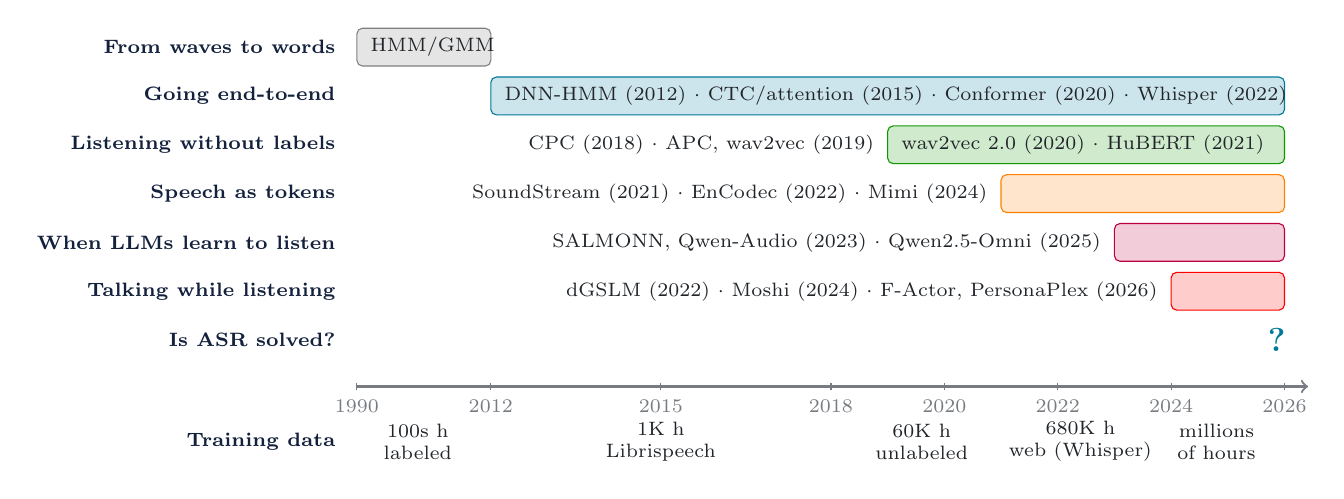
\begin{tikzpicture}[x=1cm,y=1cm]
  \era{0}{1990}{2012}{gray}{From waves to words}{HMM/GMM}
  \era{1}{2012}{2026}{accent}{Going end-to-end}{DNN-HMM (2012) $\cdot$ CTC/attention (2015) $\cdot$ Conformer (2020) $\cdot$ Whisper (2022)}
  \era{2}{2019}{2026}{LigAikumaGreen}{Listening without labels}{wav2vec 2.0 (2020) $\cdot$ HuBERT (2021)}
  \node[anchor=east, font=\scriptsize, text=ink] at (\yx{2019}-0.05,-2*0.62-0.24) {CPC (2018) $\cdot$ APC, wav2vec (2019)};
  \eraL{3}{2021}{2026}{orange}{Speech as tokens}{SoundStream (2021) $\cdot$ EnCodec (2022) $\cdot$ Mimi (2024)}
  \eraL{4}{2023}{2026}{purple}{When LLMs learn to listen}{SALMONN, Qwen-Audio (2023) $\cdot$ Qwen2.5-Omni (2025)}
  \eraL{5}{2024}{2026}{red}{Talking while listening}{dGSLM (2022) $\cdot$ Moshi (2024) $\cdot$ F-Actor, PersonaPlex (2026)}
  % open question beyond 2026
  \node[font=\scriptsize\bfseries, text=titleink, anchor=east] at (-0.15,-6*0.62-0.24) {Is ASR solved?};
  \node[font=\large\bfseries, accent] at (\yx{2026}-0.1,-6*0.62-0.24) {?};
  % time axis
  \draw[->, thick, softgrey] (0,-4.55) -- (\yx{2026}+0.3,-4.55);
  \foreach \y in {1990,2012,2015,2018,2020,2022,2024,2026}{
    \draw[softgrey] (\yx{\y},-4.5) -- (\yx{\y},-4.6);
    \node[font=\scriptsize, text=softgrey, below] at (\yx{\y},-4.6) {\y};}
  % training data scale
  \node[anchor=east, font=\scriptsize\bfseries, text=titleink] at (-0.15,-5.25) {Training data};
  \node[font=\scriptsize, text=ink, align=center] at (\yx{2000},-5.25) {100s h\\labeled};
  \node[font=\scriptsize, text=ink, align=center] at (\yx{2015},-5.25) {1K h\\Librispeech};
  \node[font=\scriptsize, text=ink, align=center] at (\yx{2019.6},-5.25) {60K h\\unlabeled};
  \node[font=\scriptsize, text=ink, align=center] at (\yx{2022.4},-5.25) {680K h\\web (Whisper)};
  \node[font=\scriptsize, text=ink, align=center] at (\yx{2024.8},-5.25) {millions\\of hours};
\end{tikzpicture}}

\end{center}
\vspace*{-0.3em}
\small
\begin{itemize}
	\item From modular pipelines to \textbf{one neural network}
	\item From transcribed speech to \textbf{raw audio at web scale}
	\item From recognizing speech to \textbf{holding a conversation}
\end{itemize}
\end{frame}


\frame{\tableofcontents}


\section{From waves to words}

\frame{\tableofcontents[currentsection]}

\begin{frame}
\frametitle{Speech facts}
\begin{itemize}
	\item Speech generally conveys a (linguistic) message (that can be reduced to a transcript)
	\item But not only (paralinguistics: speaker identity, speaker mood, speaker health condition, speaker accent, etc.) 
	\item Variability at all levels (intra speaker, inter speaker, microphone, phone line, room acoustics, style)
	\item Speech is a continuous signal (no explicit word boundaries)
	\item May be decomposed into elementary units of sound (phonemes) that distinguish one word from another in a particular language (minimal pairs)
	\begin{itemize}
		\item \textit{kill} vs \textit{kiss}  -  \textit{pat} vs \textit{bat}  
		\item phoneme set is language dependent
		\item acoustic realization of the phoneme is dependent of its left and right neighbors (co-articulation)
	\end{itemize}
\end{itemize}

\end{frame}


%%%%


\begin{frame}\frametitle{(Main) Speech tasks}

\begin{itemize}
	\item Speech compression (solved, now also with neural codecs)
	\item Speaker recognition (strong progresses over the last 10 years but still poor compared to other biometric modalities like fingerprint and iris)
	\item Text-to-speech synthesis (near-human quality and voice cloning from a few seconds of audio)
	\item \textbf{Speech-to-text and Speech-to-Speech (this talk)}
	\item Speech paralinguistics: detection of gender, age, deception, sincerity, nativeness, emotion, sleepiness, cognitive disorders, (drug or alcohol) intoxication, pathologies, etc.
	\item Main speech conference: \textit{Interspeech} (core A, every year)
\end{itemize}


\end{frame}

%%%%%


\begin{frame}\frametitle{How do we evaluate ASR? Word Error Rate (WER)}

ASR = Automatic Speech Recognition. Align the system output with the human transcript (edit distance), then count errors:
\begin{equation*}
	\text{WER} = \frac{{\color{orange}S} + {\color{red}D} + {\color{LigAikumaGreen}I}}{N}
\end{equation*}
\vspace*{-0.6em}
\begin{center}
{\small ${\color{orange}S}$: substitutions \quad ${\color{red}D}$: deletions \quad ${\color{LigAikumaGreen}I}$: insertions \quad $N$: words in reference}

\vspace*{0.6em}
\renewcommand{\arraystretch}{1.25}
\begin{tabular}{l|ccccccc}
	REF & the & cat & {\color{orange}sat} & on & the & {\color{LigAikumaGreen}--} & mat \\
	HYP & {\color{red}--} & cat & {\color{orange}sit} & on & the & {\color{LigAikumaGreen}big} & mat \\
	\hline
	    & {\color{red}\textbf{D}} & & {\color{orange}\textbf{S}} & & & {\color{LigAikumaGreen}\textbf{I}} & \\
\end{tabular}

\vspace*{0.4em}
$N=6 \Rightarrow$ WER $= (1+1+1)/6 = 50\%$
\end{center}

\vspace*{-0.2em}
\begin{itemize}
	\item WER can exceed 100\% (many insertions)
	\item No word boundaries (Chinese, Japanese, Thai)? Use the \textit{Character} Error Rate (CER)
	\item Text normalization (case, punctuation, numbers) matters a lot when comparing systems
\end{itemize}

\end{frame}

%%%%%


\begin{frame}\frametitle{Speech-to-text}

\begin{itemize}
	\item Automatic Speech Recognition (ASR): ideally spontaneous, multi-speaker, open vocabulary, any acoustic condition
	\item But performance differs greatly across contexts (read vs spontaneous ; quiet vs noisy ; native vs non-native)
\end{itemize}
\vspace*{0.3em}
		\begin{figure}
			\centering
			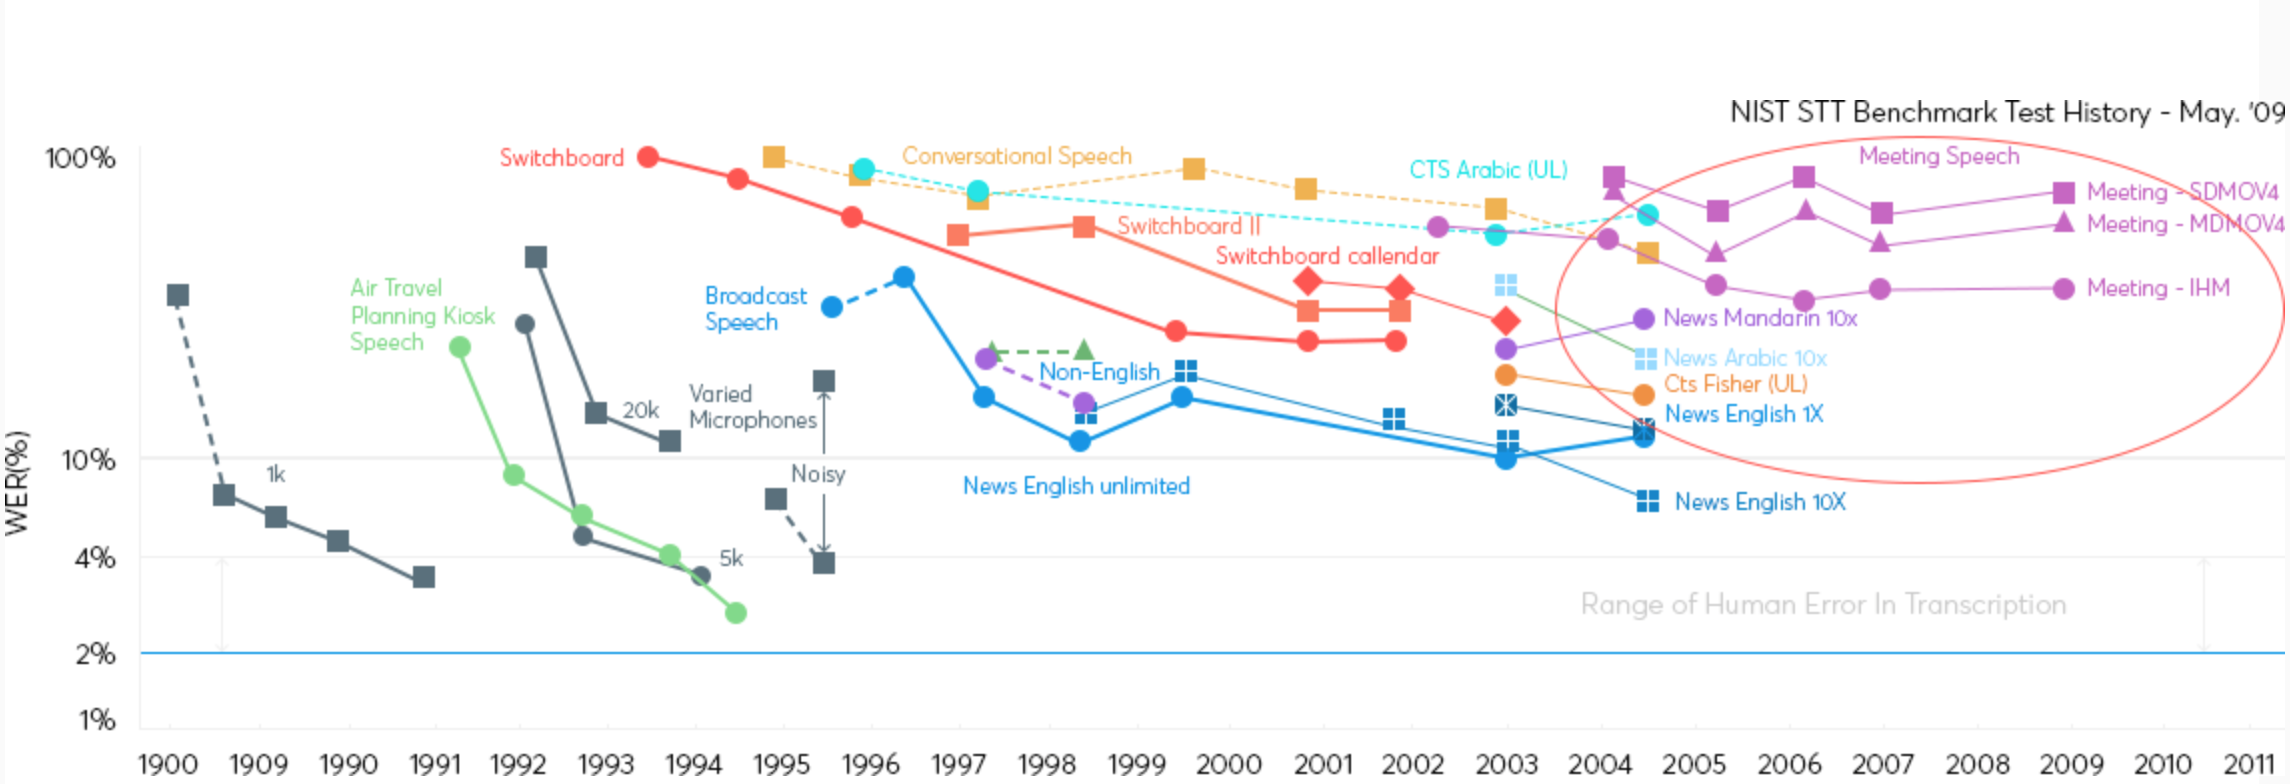
\includegraphics[width=\textwidth]{nist-history.png}
			\caption{NIST ASR benchmark tests history ($<2015$). Source: NIST}
			\label{fig:nist-history}
			\end{figure}


\end{frame}

\begin{frame}\frametitle{Speech-to-text: the Librispeech era}
		\begin{figure}
			\centering
			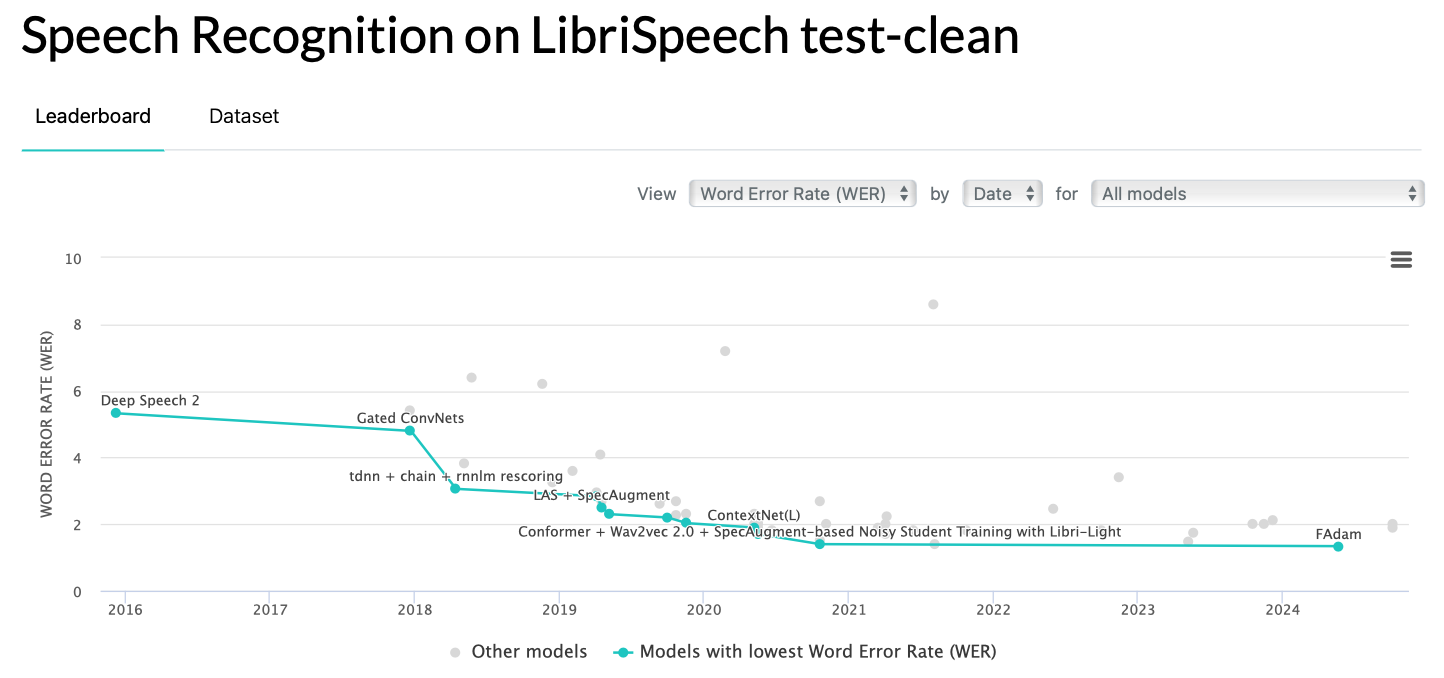
\includegraphics[width=0.95\textwidth]{librispeech-history.png}
			\caption{Librispeech ASR benchmark tests history ($>2016$). Source: \url{https://paperswithcode.com}}
			\label{fig:librispeech-history}
			\end{figure}
\end{frame}




%%%%%%%%%%%%%%%%




\begin{frame}
	\frametitle{ASR as a partial task in a larger system}

\begin{itemize}
	\item ASR for spoken language processing (speech understanding, speech translation, speech summarization, etc.)
	\item Not just a problem of noisy transcripts
	\item No sentence boundaries, punctuation, case 
	\item Disfluencies in spontaneous speech: false starts, fillers, repaired utterances
		\begin{itemize}
		\item btw, should we keep them or remove them ?
		\item some speech tasks are ill defined (ex: speech translation)
		\end{itemize}
	\item Time to work on end-to-end approaches from speech ?
\end{itemize}



	
\end{frame}

%_______________________________________________________



\begin{frame}
\frametitle{Speech representations}

\begin{columns}[T]
\begin{column}{0.58\textwidth}
\small
\begin{itemize}
	\item Handcrafted features ($<2015$)
	\begin{itemize}
		\item 20-30ms sliding windows, 10ms frame rate
		\item filterbanks, cepstral coefficients (MFCC), prosody (pitch, energy)
	\end{itemize}
	\item Spectrograms ($<1990$ and $>2015$!)
	\begin{itemize}
		\item time-frequency representation processed as an image
	\end{itemize}
	\item Raw waveform ($>2015$)
	\begin{itemize}
		\item convolutional front-end learnt with the model
	\end{itemize}
	\item Self-supervised learnt representations ($>2020$, see later!)
\end{itemize}
\end{column}
\begin{column}{0.40\textwidth}
		\begin{figure}
			\centering
			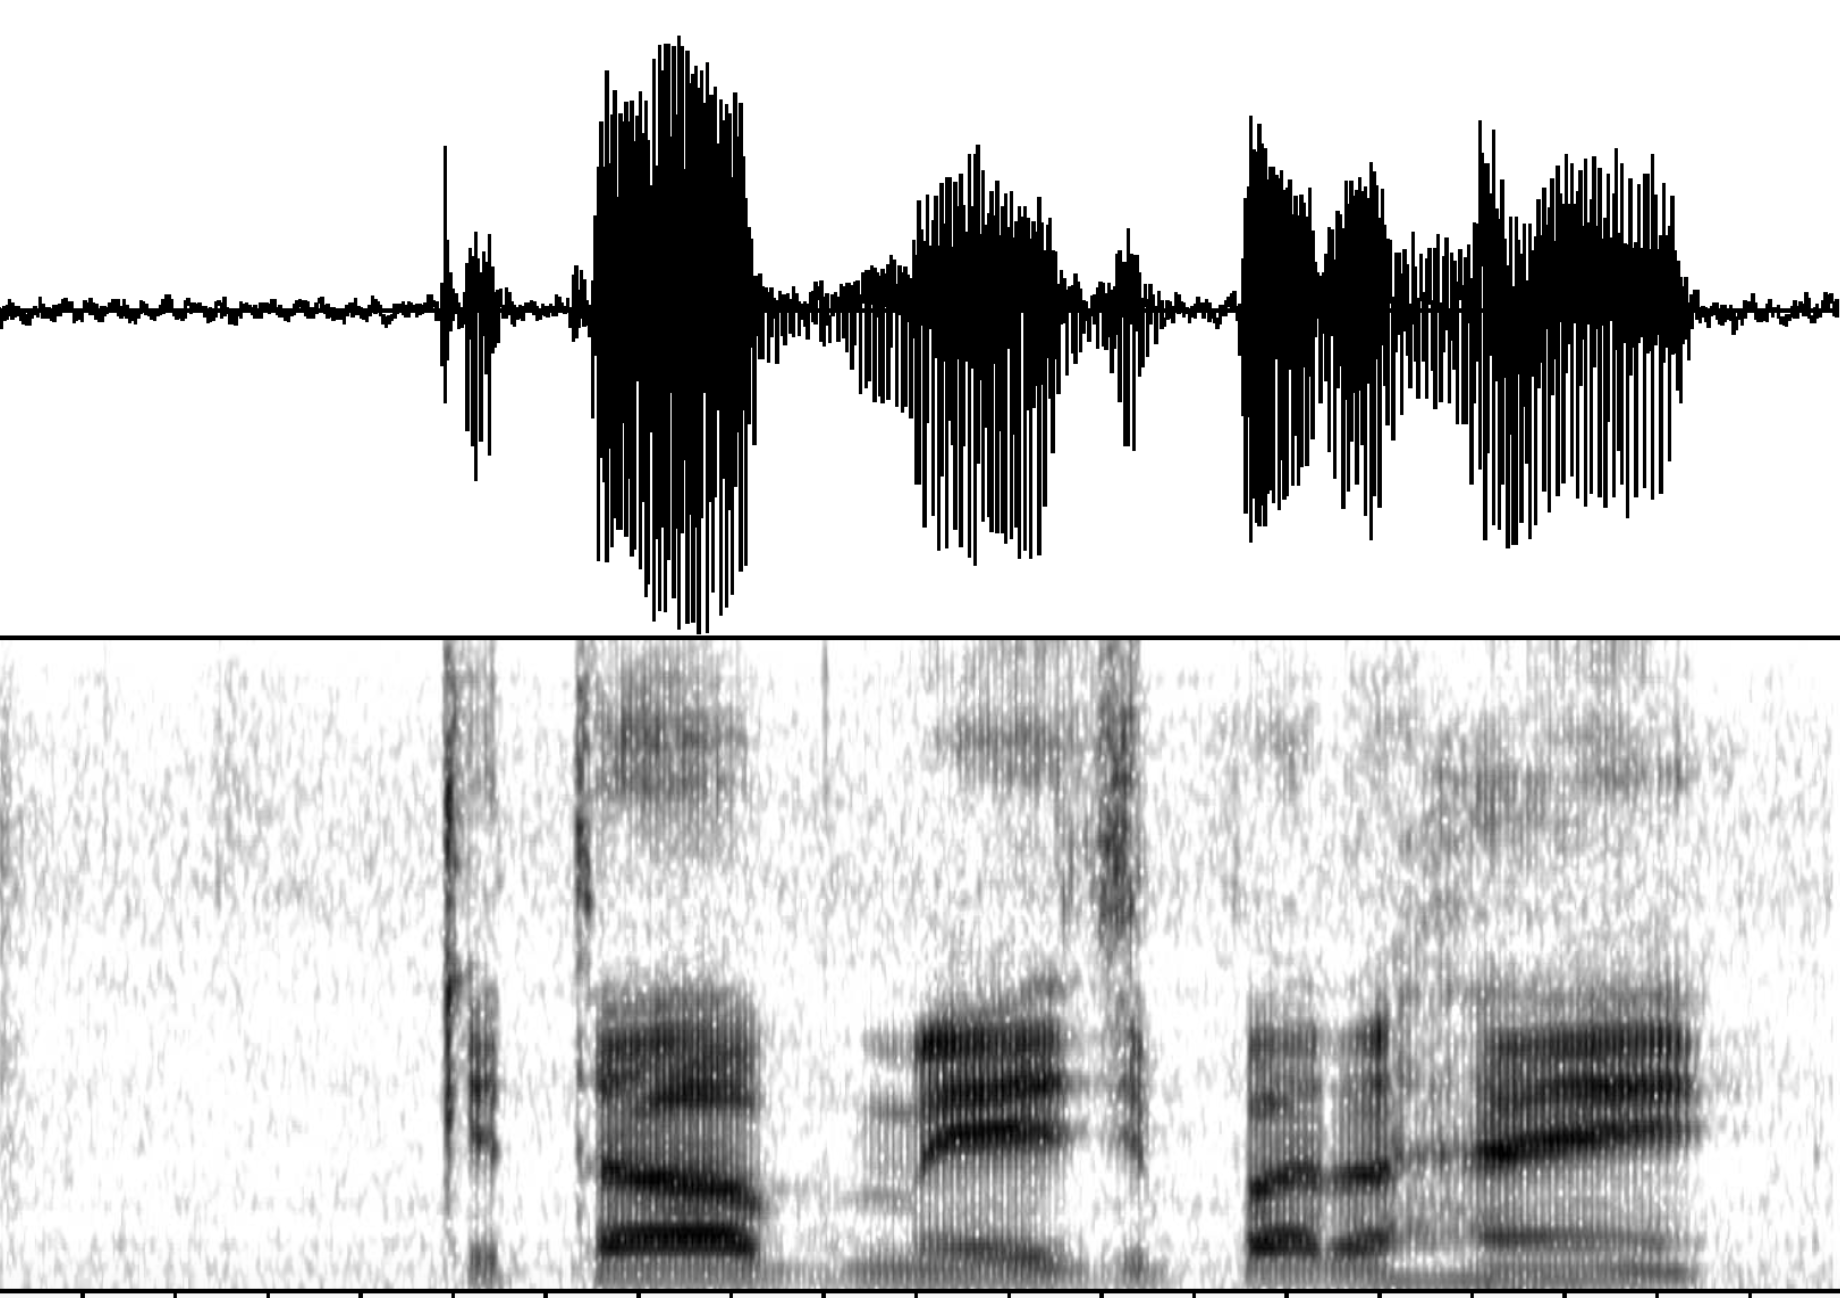
\includegraphics[width=\textwidth]{spectro.png} 
			\caption{Speech signal (top) and spectrogram (bottom)}
			\label{fig:spectro}
			\end{figure}
\end{column}
\end{columns}

\end{frame}

%%%%%%%%%%%%





\begin{frame}\frametitle{Progresses over the years}

		\begin{figure}
			\centering
			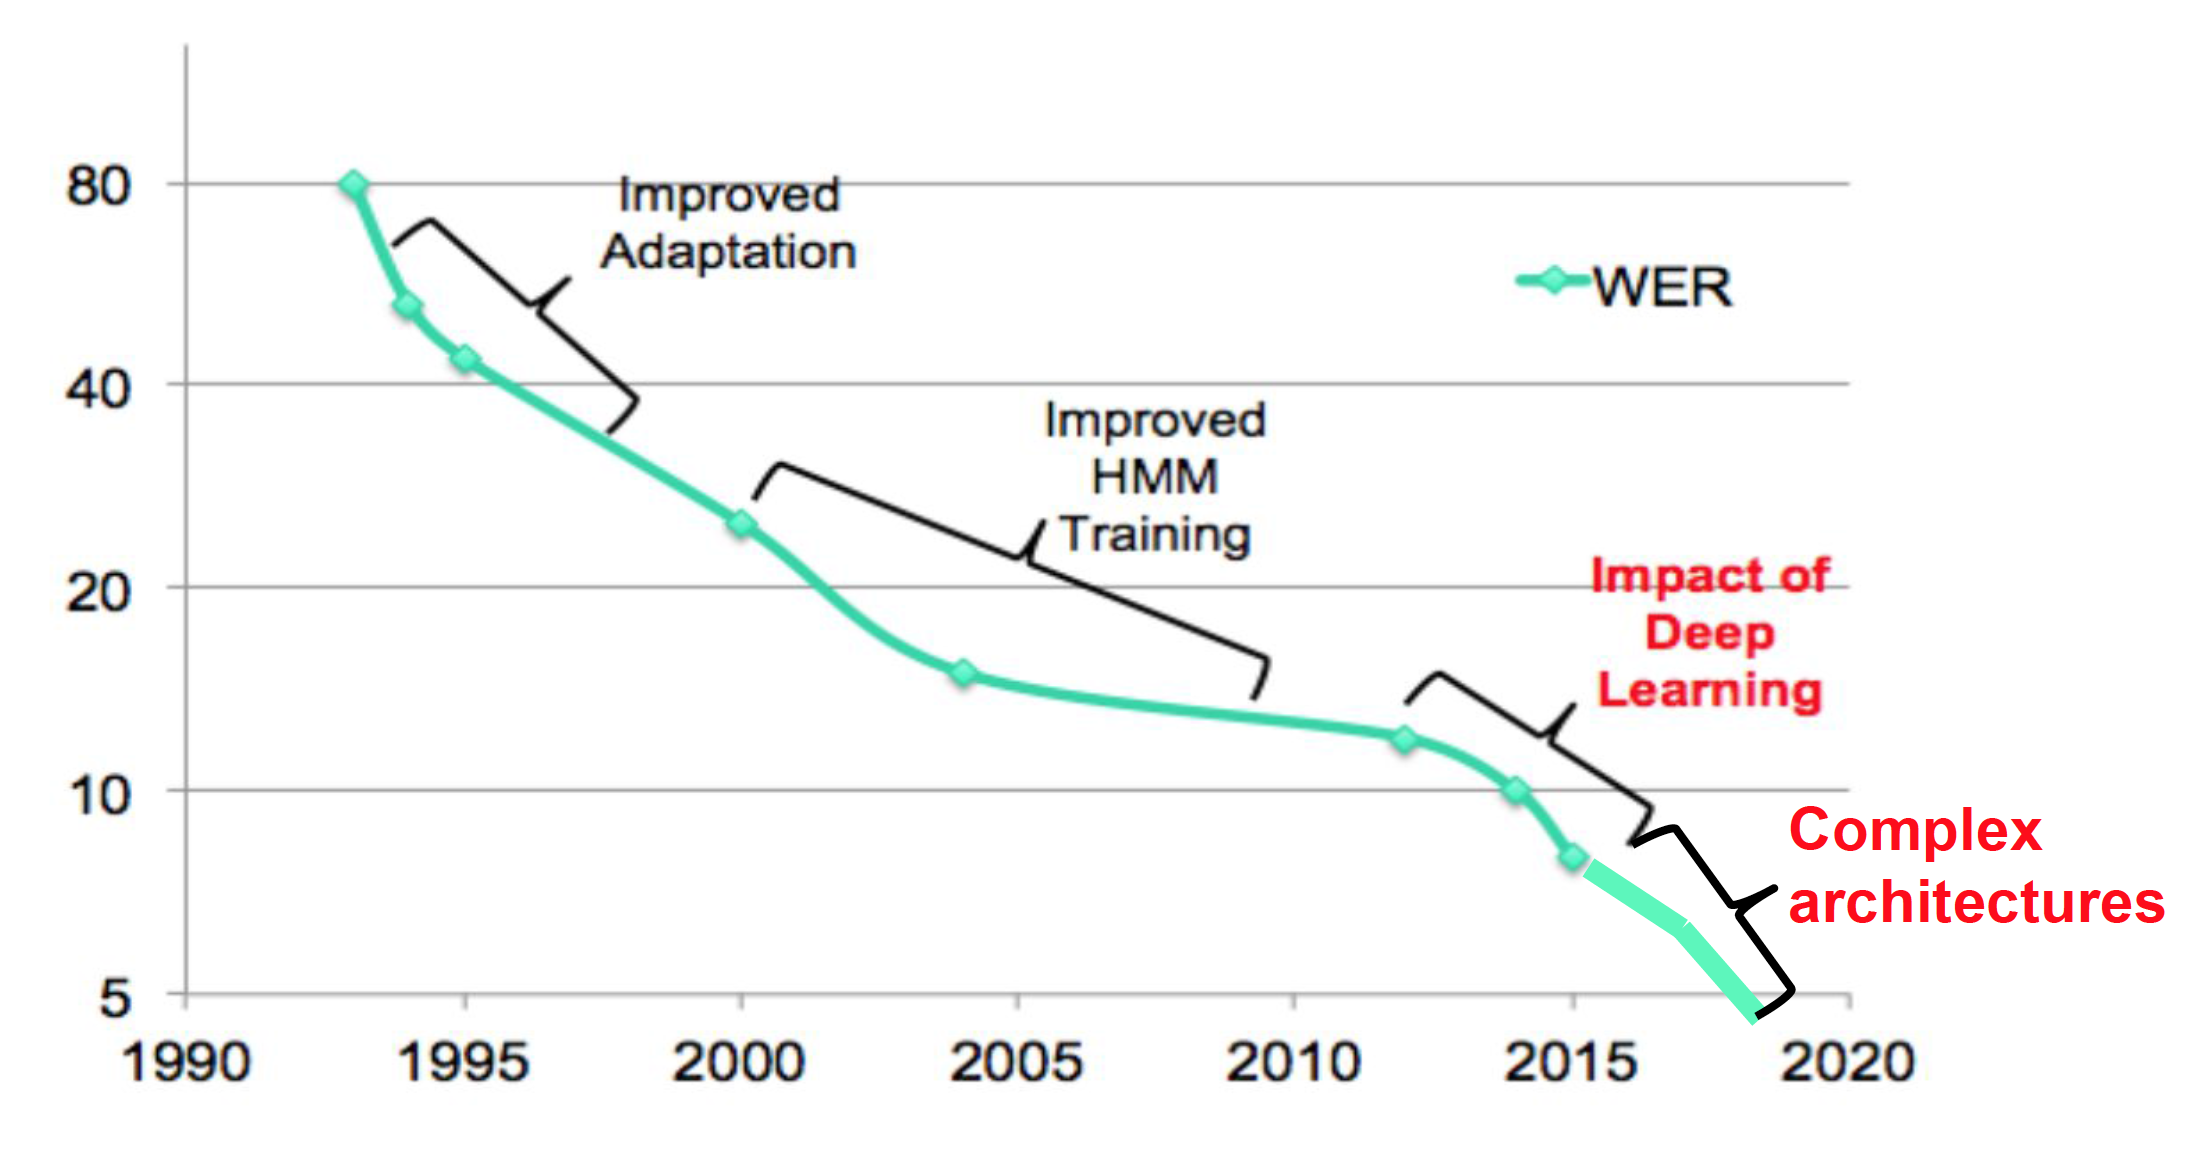
\includegraphics[scale=0.25]	{switch-conv-en.png} 
		%	[scale=0.35,trim=0mm 140mm 0mm 0mm,clip=true]
			\caption{ASR Performance\protect \footnote{Image from Bhuvana Ramabhadran' s presentation at Interspeech 2018} on English Conversational Telephony (Switchboard)}
			\label{fig:swbd}
			\end{figure}


\end{frame}


%%%%%%%%%%%%%%%%


\begin{frame}\frametitle{Classical ASR (1990-2015) in one slide}

\vspace*{-0.3em}
\begin{equation*}
   w^{*}=\arg\max_{w}p(w|x)=\arg\max_{w}{\color{red} p(x|w)}\,{\color{blue} p(w)}
\end{equation*}

\vspace*{-0.8em}
\begin{columns}[T]
\begin{column}{0.5\textwidth}
\small
\begin{itemize}
	\item {\color{red}Acoustic model $p(x|w)$}: HMMs (sequence of states) with GMMs (distribution per state), context-dependent phones (triphones)
	\item Pronunciation lexicon: words $\rightarrow$ phones ($cat$ /k a t/)
	\item {\color{blue}Language model $p(w)$}: n-grams, later RNNs
	\item Decoding: Viterbi search over the combined graph
\end{itemize}
\end{column}
\begin{column}{0.48\textwidth}
		\begin{figure}
			\centering
			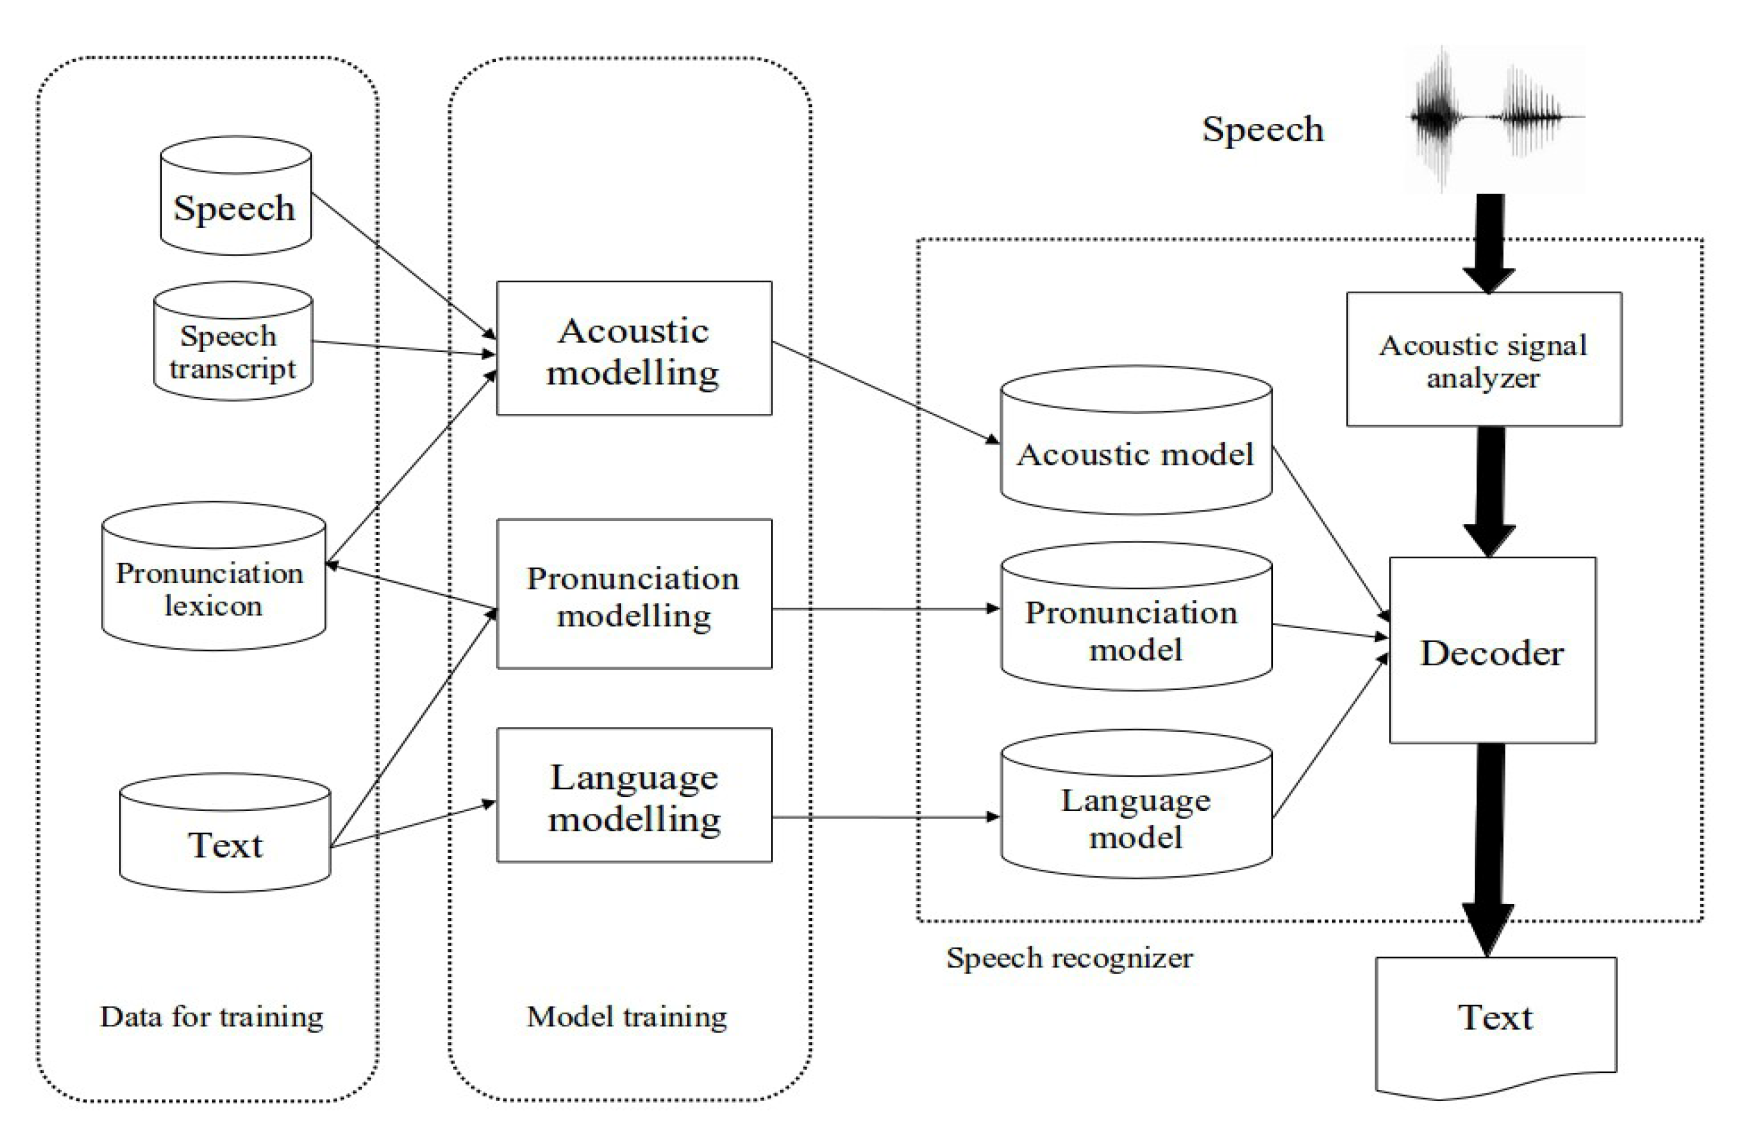
\includegraphics[width=\textwidth]{asr-global.png} 
			\caption{ASR Overview}
			\label{fig:global}
			\end{figure}
\end{column}
\end{columns}

\end{frame}



%_______________________________________________________
\quizbreak{1}{3}

\section{Going end-to-end}

\frame{\tableofcontents[currentsection]}

\begin{frame}
	\frametitle{From neural nets to deep learning (1990-2015)}
\begin{columns}[T]
\begin{column}{0.64\textwidth}
\small
	\begin{itemize}
		\item NNs used in ASR since the 90s, but slow and weaker than HMM/GMMs
		\item \textbf{Hybrid NN-HMM}: the NN estimates the posterior $p(s|x)$ of an HMM state \citep{DBLP:journals/taslp/RenalsMBCF94}
		\item \textbf{NN language models} \citep{Bengio:2003:NPL:944919.944966}, then RNN LMs \citep{mikolov10is}
		\item \textbf{2012 breakthrough}: deep NNs replace GMMs \citep{hinton2012}, like in vision, thanks to
		\begin{itemize}
			\item more data (Librispeech 1,000h in 2015 $\rightarrow$ Whisper 680,000h in 2022)
			\item GPUs, better optimization, toolkits (Kaldi \citep{Povey_ASRU2011}, PyTorch)
		\end{itemize}
	\end{itemize}
\end{column}
\begin{column}{0.34\textwidth}
		\begin{figure}
			\centering
			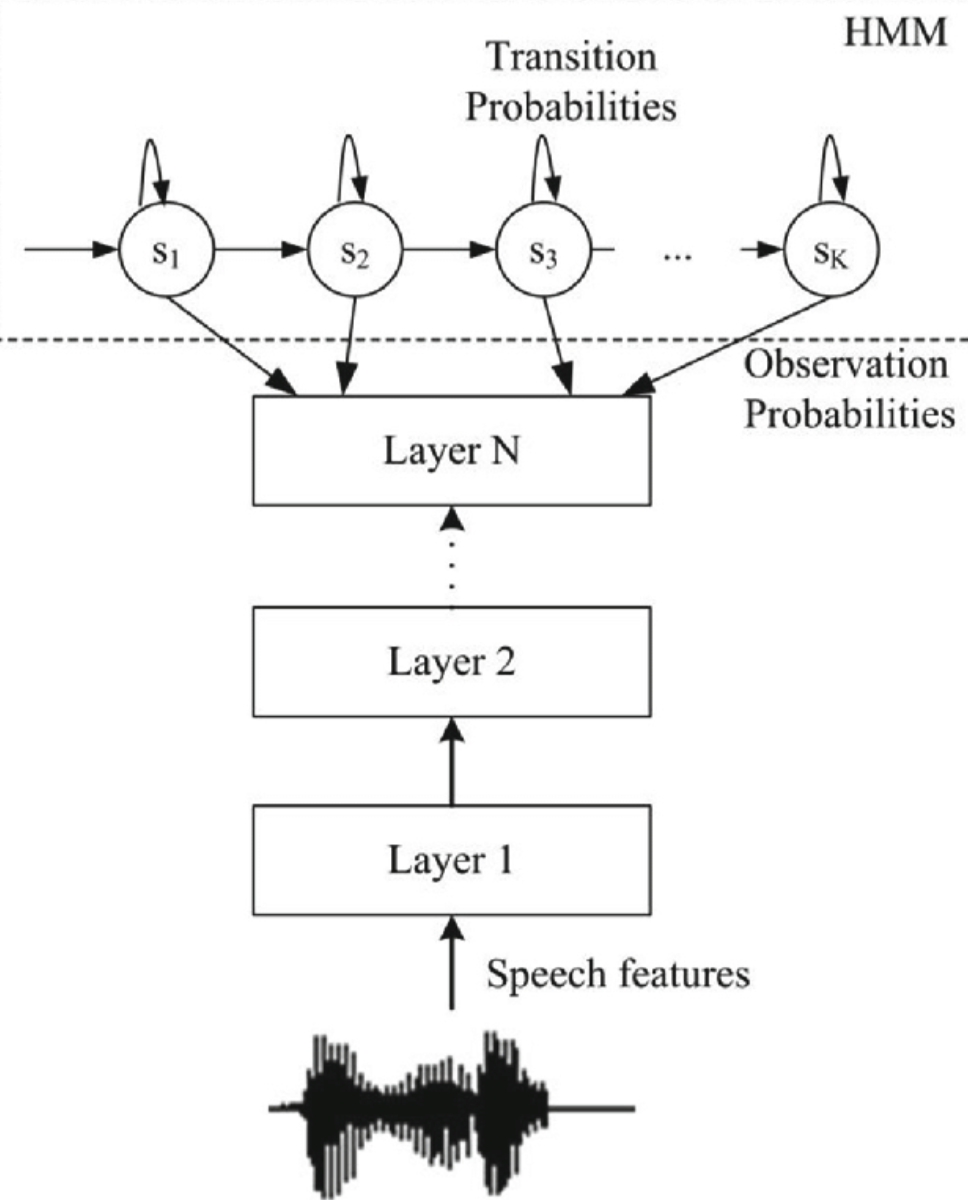
\includegraphics[width=\textwidth]{hmm-dnn.png} 
			\caption{Hybrid NN-HMM}
			\label{fig:hmm-dnn}
			\end{figure}
\end{column}
\end{columns}
\end{frame}

\begin{frame}
 \frametitle{End-to-end ASR (get rid of HMMs)}
 One neural network maps speech directly to characters, subwords or words
	\begin{itemize}
	\item Connectionist Temporal Classification (CTC)
		\begin{itemize}
		\item Solves the problem of unaligned input and output sequences by marginalizing the conditional likelihood of the output sequence given the input over all possible alignments
		\end{itemize}

	\item Attention Modeling
		\begin{itemize}
		\item Simultaneously optimize alignment and grapheme (or word) decoding using attention weights (linear combination of hidden states) to influence the generated output
		\end{itemize}
	
	\item Transducers (RNN-T) \citep{graves2012transducer}
		\begin{itemize}
		\item Encoder + prediction network (conditioned on previous outputs, like an LM) + joint network ; like CTC, marginalize over alignments with a blank symbol, but without CTC's independence assumption ; streaming-friendly
		\end{itemize}
	\end{itemize}
	
\end{frame}

%\begin{frame}
% \frametitle{CTC}
%		
%		\begin{figure}
%			\centering
%			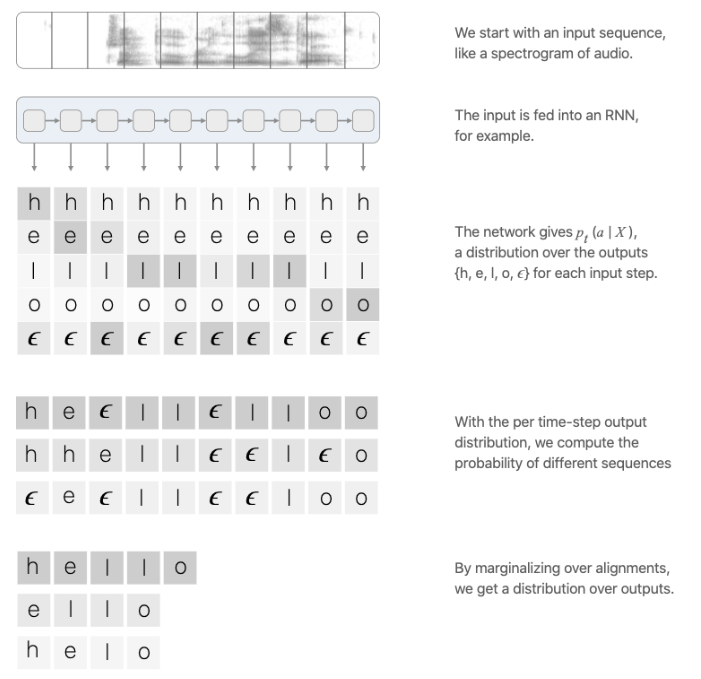
\includegraphics[scale=0.12]	{ctc12} 
%		%	[scale=0.35,trim=0mm 140mm 0mm 0mm,clip=true]
%			\caption{CTC overview\footnote{from \url{https://www.assemblyai.com/blog/end-to-end-speech-recognition-pytorch/}}
%		\end{figure}
%
%\end{frame}
%
%


\begin{frame}
 \frametitle{CTC overview}
		
		\begin{itemize}
		\item Connectionist Temporal Classification
		\item Model will learn to align the transcript itself during training \citep{DBLP:conf/icml/GravesFGS06} 
		\item Defined over a label sequence $z$ (of length M)
		\item \textit{blank or \_} symbol allows M-length target sequence to be mapped to  a T-length sequence $x$\footnote{gives the model the ability to say that a certain audio frame did not produce a character}
		\item $z$ can be represented by a set of all possible CTC paths (sequence of labels, at frame level) that are mapped to $z$
				\begin{itemize}
				\item ex: M=2 ($z=hi$) and T=3 (3 frames): possible sequences are 'hhi', 'hii', '\_hi', 'h\_i', 'hi\_' 
				\end{itemize}
		\item Probability $p(z/x)$ evaluated as sum of probabilities over all possible CTC paths (using Forward-Backward)
		\item Generate frame posteriors at decoding time
		\end{itemize}

\end{frame}


\begin{frame}
 \frametitle{CTC loss function}
		\begin{figure}
			\centering
			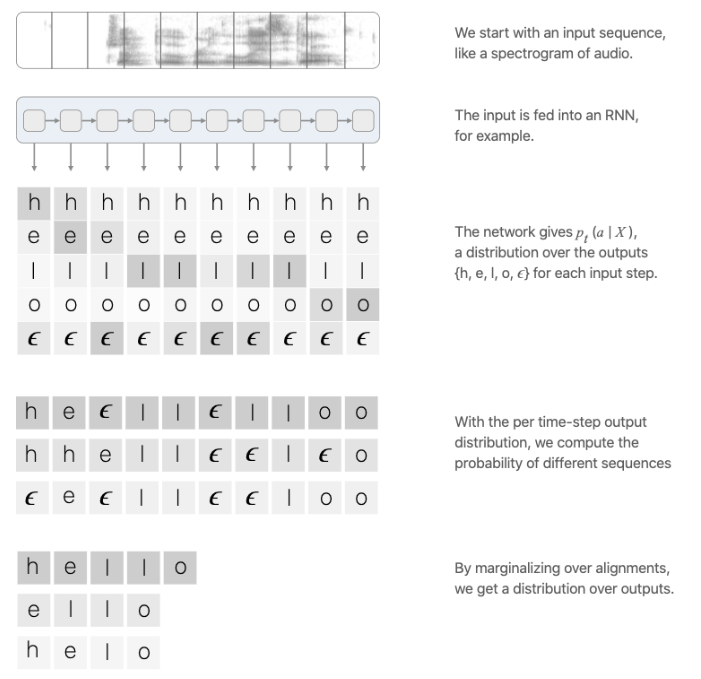
\includegraphics[scale=0.22]	{ctc12.png} 
			\caption{CTC Overview {\tiny (from \url{https://www.assemblyai.com/blog/end-to-end-speech-recognition-pytorch})}}
			\end{figure}
		\vspace*{-0.5em}
		\begin{itemize}
		\item There can be a massive number of alignments, so the loss is computed with dynamic programming (forward-backward)
		\end{itemize}
\end{frame}


\begin{frame}
 \frametitle{CTC inference}
		
		\begin{itemize}
		\item Greedy decoding
		\begin{figure}
			\centering
			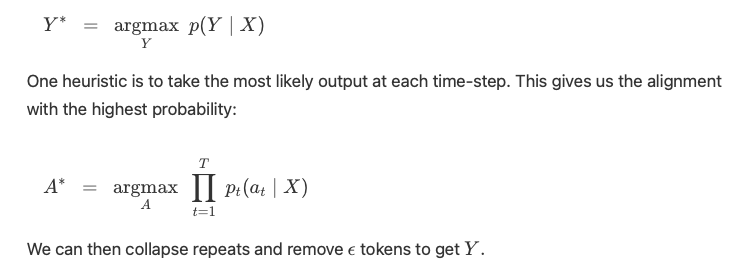
\includegraphics[scale=0.24]	{ctcinference.png} 
		\end{figure}
		\item Beam-Search decoding
		\begin{figure}
			\centering
			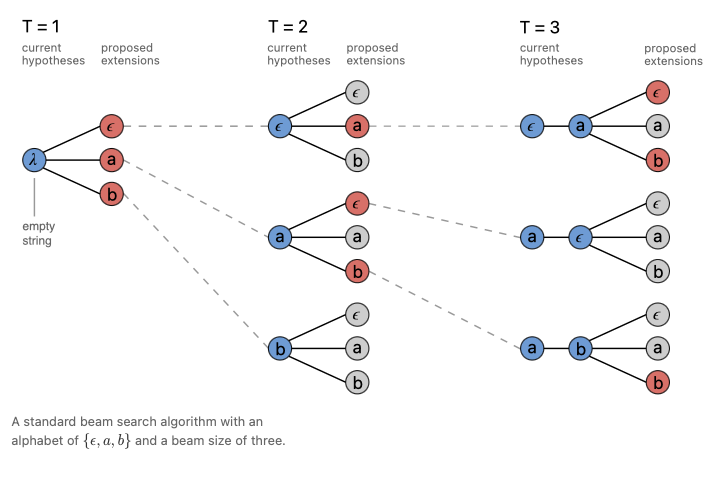
\includegraphics[scale=0.17]	{ctcbs.png} 
			\caption{from  \url{https://www.assemblyai.com/blog/end-to-end-speech-recognition-pytorch}}
		\end{figure}

		\end{itemize}

\end{frame}


%%%%%%%%%%%%%%%%%%%%
\begin{frame}
 \frametitle{Attention modeling}
Initially proposed for (neural) machine translation \citep{DBLP:journals/corr/BahdanauCB14} and introduced for ASR by \cite{DBLP:journals/corr/ChorowskiBSCB15}
\begin{columns}[T]
\begin{column}{0.55\textwidth}
\small
	\begin{itemize}
	\item A speech encoder (CNNs, pyramidal LSTMs \cite{chorowski2015attention}, now Transformers)
	\item A context (attention) model is a function of the encoder codes and of the previous decoded tokens
	\item While CTC generates frame-level posteriors, attention models generate L predictions until the end-of-sequence symbol (no posterior for a given frame)
	\end{itemize}
\end{column}
\begin{column}{0.43\textwidth}
\begin{center}
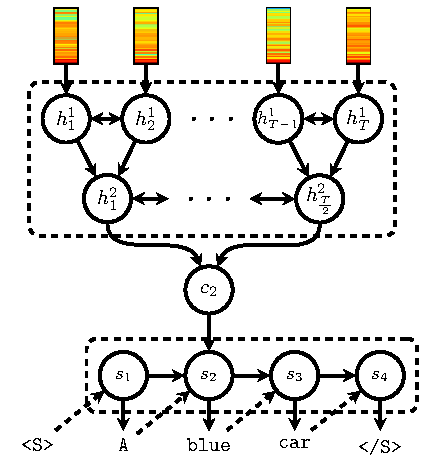
\includegraphics[width=\textwidth]{pyramidal}

\tiny Image from Alexandre Berard's thesis
\end{center}
\end{column}
\end{columns}
\end{frame}


%%%%%%%%%%%%%%%%%%%%
\begin{frame}
\frametitle{Attention modeling: listen, attend and spell}
\begin{columns}[T]
\begin{column}{0.49\textwidth}
\small
\begin{itemize}
  \item \textbf{L}isten (encode), \textbf{A}ttend, \textbf{S}pell (decode, one token at a time)
\end{itemize}
\begin{center}
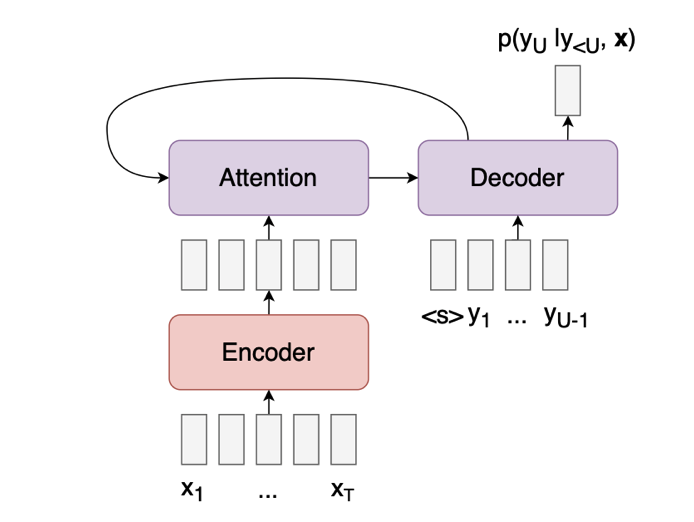
\includegraphics[width=\textwidth]{attentionmodels.png}
\end{center}
\end{column}
\begin{column}{0.49\textwidth}
\small
\begin{itemize}
  \item Attention weights give a soft alignment between output tokens and input frames, possibly non-monotonic (CTC is monotonic)
\end{itemize}
\begin{center}
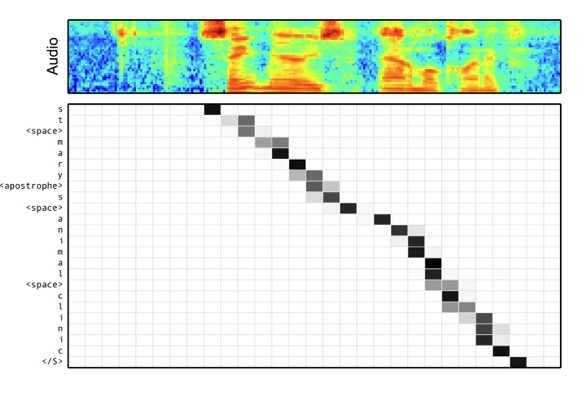
\includegraphics[width=\textwidth]{alignment2.png}
\end{center}
\end{column}
\end{columns}
\begin{center}
\tiny Images from \url{https://lorenlugosch.github.io/posts/2020/11/transducer/}
\end{center}
\end{frame}
%%%%%%%%%%%%%%%%%%%%


% --- old attention slides (different view, alignment) merged above ---
%\begin{frame}
%\frametitle{Attention modeling (different view)}
%\begin{itemize}
%  \item Also called LAS: \textbf{L}isten (encode) ; \textbf{A}ttend (attention) and \textbf{S}pell (decode)
%\end{itemize}
%\begin{center}
%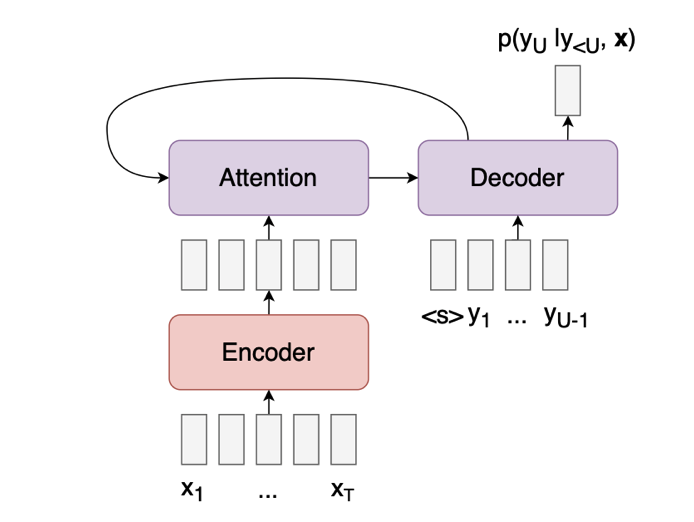
\includegraphics[width=.45\linewidth]{attentionmodels.png}
%
%\tiny Image from \url{https://lorenlugosch.github.io/posts/2020/11/transducer/}
%\end{center}
%\end{frame}
%\begin{frame}
%\frametitle{Attention modeling (alignment)}
%\begin{itemize}
%  \item Allows non-monotonic alignements
%  \item As opposed to CTC (monotonic)
%\end{itemize}
%\begin{center}
%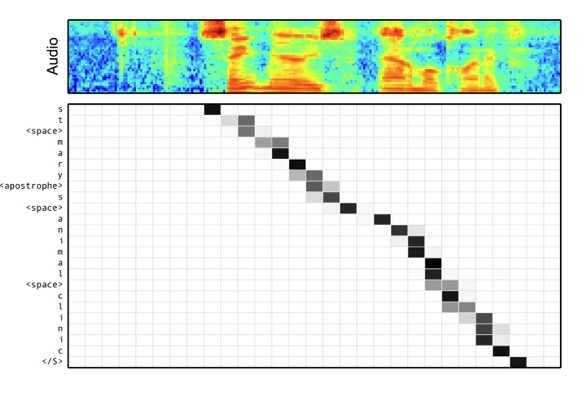
\includegraphics[width=.45\linewidth]{alignment2.png}
%
%\tiny Image from \url{https://lorenlugosch.github.io/posts/2020/11/transducer/}
%\end{center}
%\end{frame}
%%%%%%%%%%%%%%%%%%%%


\begin{frame}
\frametitle{CTC versus Attention}
\begin{itemize}
  \item CTC provides monotonic alignements while attention allows non-monotonic alignements
  	\begin{itemize}
		\item Attention more suitable for speech translation
	\end{itemize}
  \item Attention will induce Auto-Regressive decoding (one token at a time) as attention depends on decoder's state
  	\begin{itemize}
	 	\item slow inference
	\end{itemize}
  \item CTC does not have this constraint and is much simpler
  	\begin{itemize}
		\item faster inference
	\end{itemize}
  \item In practice, both are often combined (joint CTC/attention training and decoding)
  \item Transducers (RNN-T): alignment-free like CTC, but each output also depends on previous outputs through a prediction network ; streaming, on-device, and among the fastest accurate models today (e.g., token-and-duration transducers \citep{xu2023tdt})
\end{itemize}
\end{frame}
%%%%%%%%%%%%%%%%%%%


\begin{frame}
\frametitle{The Conformer encoder}
\begin{columns}[T]
\begin{column}{0.44\textwidth}
\small
\begin{itemize}
	\item Convolution-augmented Transformer \citep{conformer}
	\item Attention: \textit{global} context ; convolution: \textit{local} patterns
	\item Subsampling: 10ms $\rightarrow$ 40ms frames (80ms in FastConformer)
	\item Default ASR encoder since 2020, for any decoder (CTC, transducer, attention, LLM)
\end{itemize}
\end{column}
\begin{column}{0.55\textwidth}
\begin{figure}
	\centering
	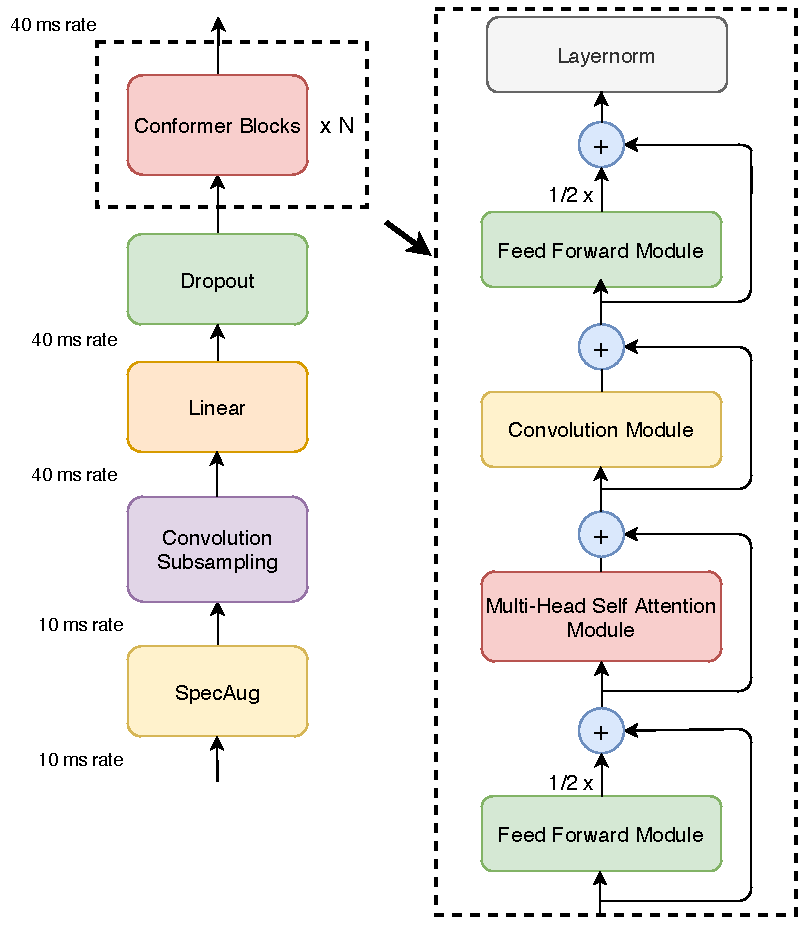
\includegraphics[height=5.6cm]{images2026/conformer-gulati2020.png}
	\caption{Figure from \citep{conformer}}
\end{figure}
\end{column}
\end{columns}
\end{frame}


%%%WHISPER
\begin{frame}
	\frametitle{Whisper: large-scale weak supervision}
\begin{columns}[T]
\begin{column}{0.55\textwidth}
		\small
		\begin{itemize}
			\item Massively multilingual ASR based on weakly-supervised learning \citep{whisper}
			\item 680,000 hours of web data (large-v3: 1M hours weakly labeled + 4M hours pseudo-labeled by large-v2) $\rightarrow$ robust to accents, noise and technical language
			\item One model, many tasks selected by special tokens: transcription (99 languages), translation into English, language ID, timestamps
			\item Simple encoder-decoder Transformer: the de facto baseline (and encoder) for many systems since 2022
		\end{itemize}
\end{column}
\begin{column}{0.43\textwidth}
		\begin{center}
			\vspace*{1em}
			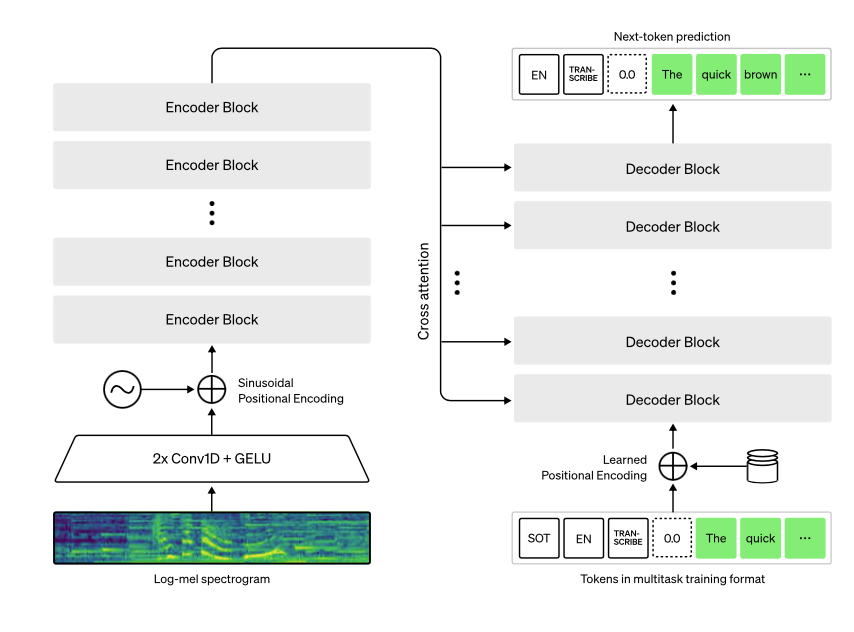
\includegraphics[width=\textwidth]{whisper.png}\\
			{\footnotesize\color{softgrey} Figure from \citep{whisper}}
		\end{center}
\end{column}
\end{columns}
\end{frame}


\begin{frame}
	\frametitle{Open multilingual ASR models}
	\small
	\begin{itemize}
		\item OWSM: Whisper-style training reproduced with public data and an open toolkit (ESPnet) \citep{peng2023owsm}
		\item MMS: 1,100+ languages (religious recordings, wav2vec 2.0) \citep{pratap2023mms}
		\item Omnilingual ASR: 1,600+ languages, 500+ never covered before, new languages added from a few examples (in-context) \citep{omnilingual2025}
		\item mHuBERT-147: compact (95M) multilingual SSL encoder, 147 languages, 90K hours of open data \citep{zanonboito2024mhubert}
	\end{itemize}
	\begin{figure}
		\centering
		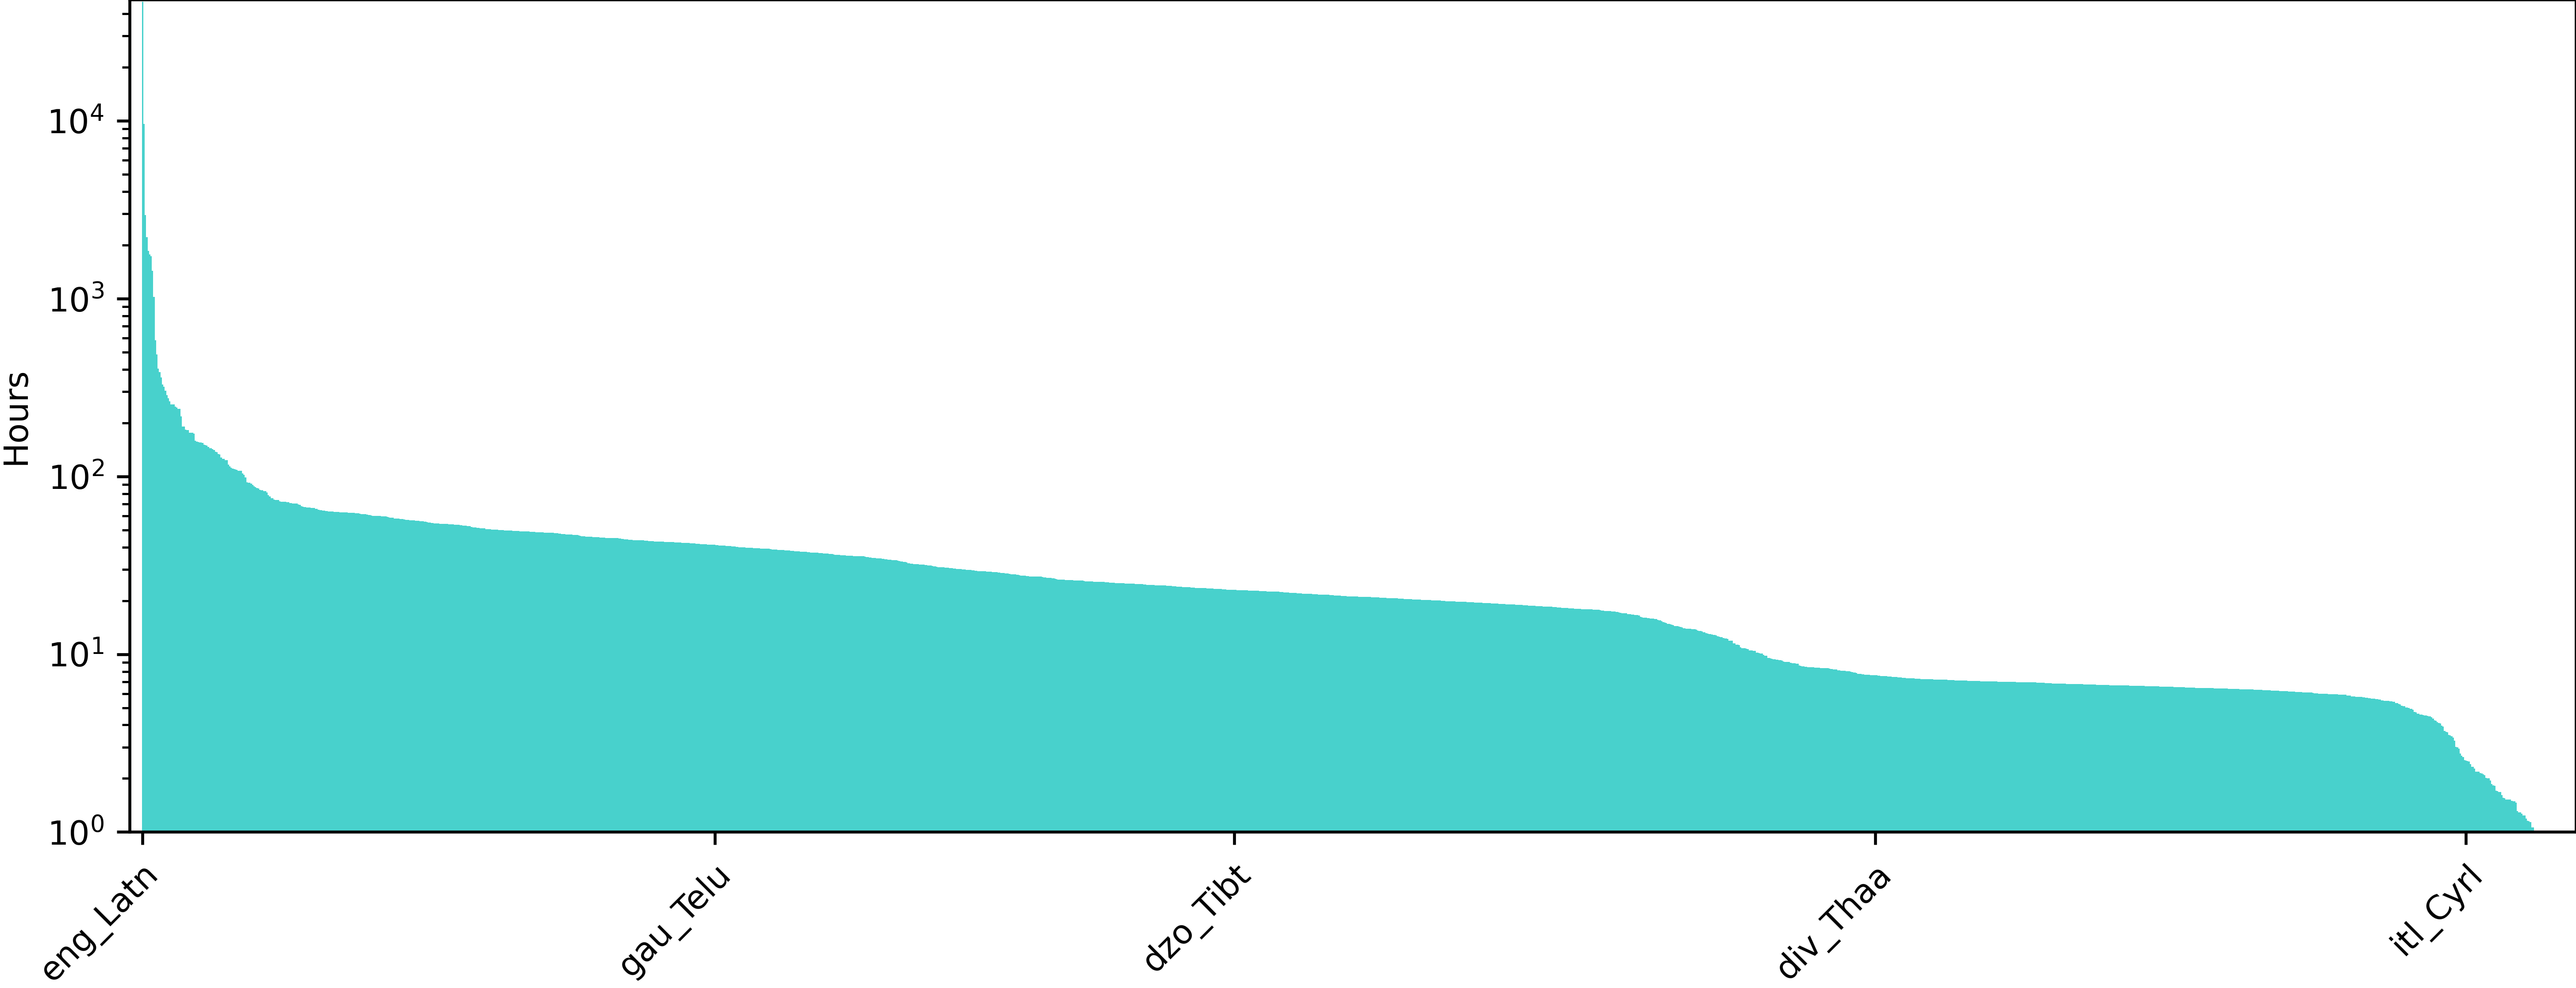
\includegraphics[height=2.1cm]{images2026/omnilingual-hours-per-lang.png}
		\caption{Labeled hours per language (log): a long tail \citep{omnilingual2025}}
	\end{figure}
\end{frame}


\begin{frame}
	\frametitle{Comparing systems: the Open ASR Leaderboard}
{\small 60+ systems evaluated on 11 English test sets with the same text normalization}

\vspace*{-0.2em}
\begin{center}
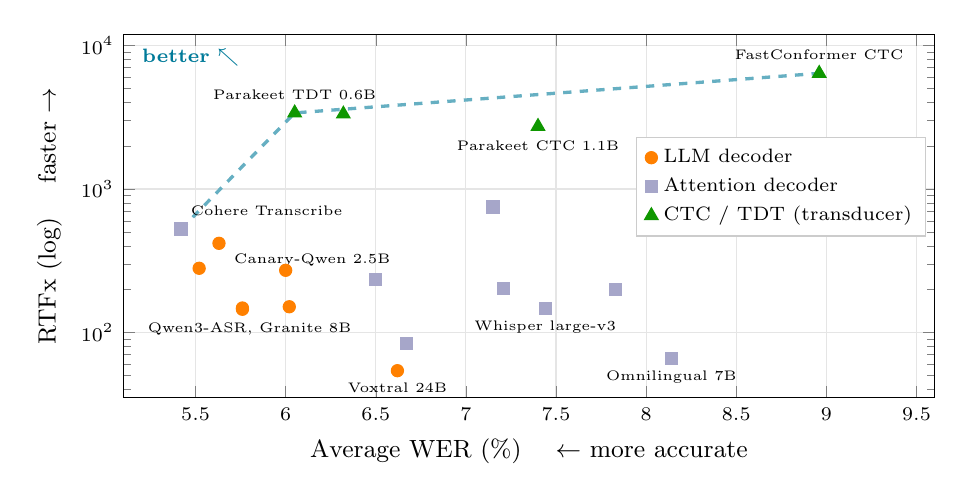
\begin{tikzpicture}
\begin{axis}[
  width=0.98\textwidth, height=6.2cm,
  ymode=log, xmin=5.1, xmax=9.6, ymin=35, ymax=12000,
  xlabel={\small Average WER (\%) \quad $\leftarrow$ more accurate},
  ylabel={\small RTFx (log) \quad faster $\rightarrow$},
  tick label style={font=\scriptsize},
  label style={font=\small},
  grid=major, grid style={gray!20},
  legend style={font=\scriptsize, at={(0.99,0.58)}, anchor=east, draw=gray!40},
  legend cell align=left,
  every node near coord/.append style={font=\tiny},
]
% Pareto frontier (computed on the models shown)
\addplot[accent!60, dashed, very thick, forget plot] coordinates {(5.42,525) (6.05,3390) (8.96,6400)};
% LLM decoders
\addplot[only marks, mark=*, mark size=2.2pt, color=orange] coordinates {(5.52,280) (5.63,418) (5.76,145) (5.76,148) (6.00,271) (6.02,151) (6.62,54.1)};
\addlegendentry{LLM decoder}
% Attention (encoder-decoder) decoders
\addplot[only marks, mark=square*, mark size=2.2pt, color=blue!70] coordinates {(5.42,525) (6.50,235) (6.67,84.1) (7.15,749) (7.21,202) (7.44,146) (7.83,200) (8.14,66.0)};
\addlegendentry{Attention decoder}
% CTC / TDT decoders
\addplot[only marks, mark=triangle*, mark size=2.8pt, color=LigAikumaGreen] coordinates {(6.05,3390) (6.32,3330) (7.40,2730) (8.96,6400)};
\addlegendentry{CTC / TDT (transducer)}
% labels
\node[font=\tiny, anchor=south west] at (axis cs:5.42,560) {Cohere Transcribe};
\node[font=\tiny, anchor=north west] at (axis cs:5.66,410) {Canary-Qwen 2.5B};
\node[font=\tiny, anchor=north] at (axis cs:5.80,135) {Qwen3-ASR, Granite 8B};
\node[font=\tiny, anchor=south] at (axis cs:6.05,3600) {Parakeet TDT 0.6B};
\node[font=\tiny, anchor=north] at (axis cs:7.40,2550) {Parakeet CTC 1.1B};
\node[font=\tiny, anchor=south] at (axis cs:8.96,6800) {FastConformer CTC};
\node[font=\tiny, anchor=north] at (axis cs:7.44,140) {Whisper large-v3};
\node[font=\tiny, anchor=north] at (axis cs:6.62,52) {Voxtral 24B};
\node[font=\tiny, anchor=north] at (axis cs:8.14,63) {Omnilingual 7B};
\node[font=\scriptsize, accent, anchor=north west] at (axis cs:5.15,11000) {\textbf{better} $\nwarrow$};
\end{axis}
\end{tikzpicture}
\end{center}
\vspace*{-0.6em}
{\scriptsize RTFx: seconds of audio transcribed per second of compute (1000 = 1h in 3.6s). Dashed: Pareto frontier.\\ Data from \citep{srivastav2025openasr} (arXiv v4, March 2026), open models only.\par}
\end{frame}


\begin{frame}
	\frametitle{Building an ASR system in 2026}
\begin{center}
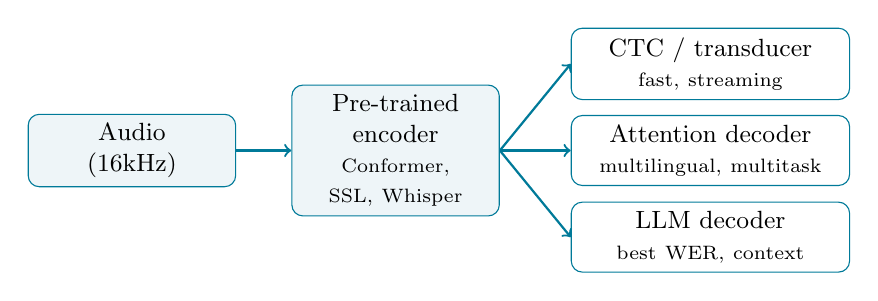
\begin{tikzpicture}[node distance=0.5cm, every node/.style={font=\small},
  box/.style={draw=accent, rounded corners, fill=blockbg, minimum height=0.9cm, align=center, text width=2.4cm},
  dec/.style={draw=accent, rounded corners, fill=white, minimum height=0.8cm, align=center, text width=3.3cm}]
  \node[box] (audio) {Audio\\(16kHz)};
  \node[box, right=0.7cm of audio] (enc) {Pre-trained encoder\\{\scriptsize Conformer, SSL, Whisper}};
  \node[dec, right=0.9cm of enc, yshift=1.1cm] (ctc) {CTC / transducer\\{\scriptsize fast, streaming}};
  \node[dec, right=0.9cm of enc] (att) {Attention decoder\\{\scriptsize multilingual, multitask}};
  \node[dec, right=0.9cm of enc, yshift=-1.1cm] (llm) {LLM decoder\\{\scriptsize best WER, context}};
  \draw[->, thick, accent] (audio) -- (enc);
  \draw[->, thick, accent] (enc.east) -- (ctc.west);
  \draw[->, thick, accent] (enc.east) -- (att.west);
  \draw[->, thick, accent] (enc.east) -- (llm.west);
\end{tikzpicture}

\end{center}
\begin{itemize}
	\item \textbf{Data}: large-scale weakly labeled and pseudo-labeled speech matters as much as the model
	\item \textbf{Decoder}: depends on the use case (latency, languages, need for context)
	\item \textbf{Evaluation}: normalized WER on diverse test sets, plus speed (RTFx)
	\item LLM decoders (speech LLMs) are covered later in this course
\end{itemize}
\end{frame}


%_______________________________________________________



%%%INTRO
\quizbreak{2}{3}

\section{Listening without labels (SSL)}

\frame{\tableofcontents[currentsection]}

\begin{frame}
\frametitle{Self supervised representation learning}
\begin{itemize}
	\item Using huge unlabeled data for training ; targets are computed from the signal itself
		\begin{itemize}
		\item \textit{''learn representations using objective functions similar to those used for supervised learning, but train networks to perform pretext tasks where both the inputs and labels are derived from an unlabeled dataset''} (from \cite{norouzi} )
		\end{itemize}
	\item Introduced for vision: see for instance  \citep{norouzi} 
	\begin{itemize}
		\item learn representations by contrasting positive pairs against negative pairs
	\end{itemize}
	\item Introduced also in NLP: see for instance \citep{bert}
	\begin{itemize}
		\item learn representations by predicting tokens that were masked in an input sequence
	\end{itemize}
\end{itemize}

\end{frame}

\begin{frame}
\frametitle{Previous works}
\begin{itemize}
	\item Stacked restricted Boltzman machines (RBM) \citep{HinSal06}
		\begin{itemize}
		\item hidden layer extracts relevant features from the observations that serve as input to next RBM that is stacked on top of it forming a deterministic feed-forward neural network
		\end{itemize}
	\item Denoising autoencoders (AE) \citep{Vincent08extractingand}
		\begin{itemize}
		\item networks which are tasked with reconstructing outputs from their (noisy) input versions
		\end{itemize}
	\item Variational autoencoders (VAE) \citep{kingma2013autoencoding}
		\begin{itemize}
		\item VAE is like a traditional AE in which the encoder produces distributions over latent representations (rather than deterministic encodings) while the decoder is trained on samples from this distribution
		\item both encoder and decoder are trained jointly
		\item VQ-VAE \citep{NIPS2017_7210} replaces continuous latent vectors with deterministically quantized versions
		\end{itemize}
\end{itemize}

\end{frame}

\begin{frame}
\frametitle{Pre-trained language models}
	\begin{itemize}
		\item Leverage large amount of freely available unlabeled text to facilitate transfer learning in NLP
		\item Yield state-of-the-art results on a wide range of NLP tasks + save time and computational resources
		\item Example of BERT \citep{bert} based on the Transformer model \citep{Vaswani2017}
	\end{itemize}
	
\begin{center}
	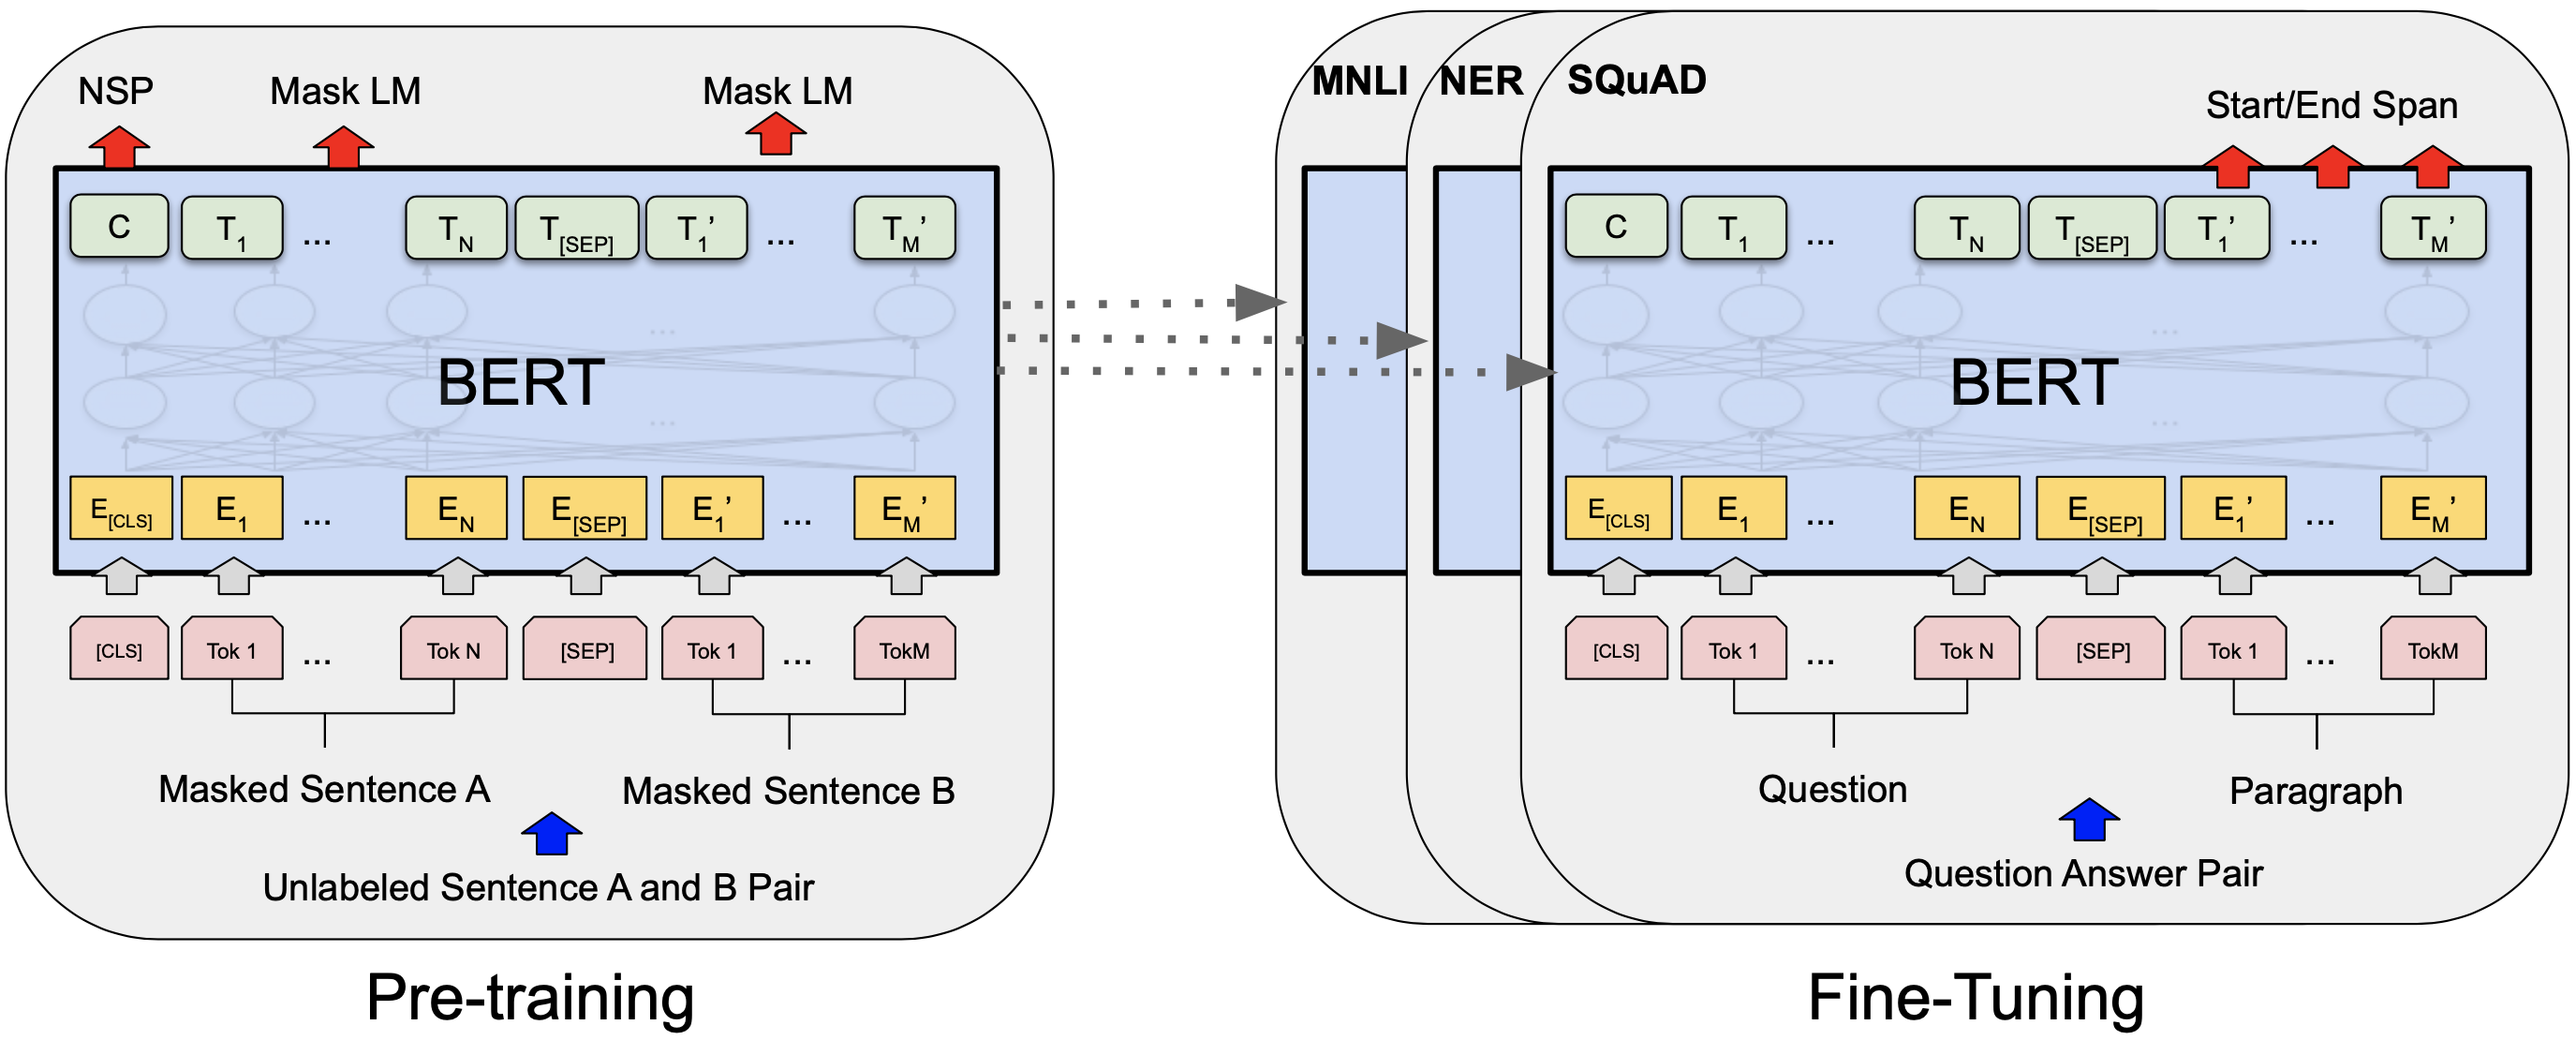
\includegraphics[width=0.8\textwidth]{bert_finetune}

	{\footnotesize\color{softgrey} Figure from \citep{bert}}
\end{center}

\end{frame}

\begin{frame}
\frametitle{Self supervised representation learning from speech}
Three families of pretext tasks
\begin{itemize}
	\item \textbf{Predictive}: predict future frames
		\begin{itemize}
		\item Autoregressive predictive coding (APC) \citep{DBLP:journals/corr/abs-1904-03240,chung2020improved}
		\end{itemize}
	\item \textbf{Contrastive}: distinguish the true (future or masked) frame from negatives
		\begin{itemize}
		\item Contrastive Predictive Coding (CPC) \citep{CPCfirstref}, wav2vec \citep{DBLP:journals/corr/abs-1904-05862}, wav2vec 2.0 \citep{DBLP:conf/nips/BaevskiZMA20}
		\end{itemize}	
	\item \textbf{Masked prediction}: predict (discrete) targets of masked frames, like BERT
		\begin{itemize}
		\item HuBERT \citep{DBLP:journals/corr/abs-2106-07447}, WavLM \citep{chen2022wavlm}, w2v-BERT \citep{chung2021w2vbert}, data2vec \citep{baevski2022data2vec}
		\end{itemize}
\end{itemize} 
\end{frame}


\begin{frame}
\frametitle{Autoregressive predictive coding (APC)}
\begin{itemize}
\item Predicting the spectrum of a future frame (rather than a wave sample) \citep{DBLP:journals/corr/abs-1904-03240} 
\item Somewhat inspired by language models (LMs) for text, which are typically a probability distribution over sequences of T tokens $(t_1,t_2,...,t_T )$
\begin{equation}
	P(sequence) = \prod_{k=1}^{T} P(t{_{k}}|t{_{1}},t{_{2}},...,t{_{k-1}})
\end{equation}
\begin{equation}
	P(sequence) = \prod_{k=1}^{T} P(t{_{k}}|h)
\end{equation}
\item Recurrent neural network LM: $h=rnn\_state(E(t{_{1}}),E(t{_{2}}),...,E(t{_{k-1}}))$
\item For speech, each token $t_k$ corresponds to a frame rather than a word or character token
\end{itemize} 
\end{frame}

\begin{frame}
\frametitle{Autoregressive predictive coding (APC)}
		\begin{itemize}
			\item No final set of target tokens (softmax layer replaced by a regression layer)
			\item Learnable parameters in APC are the RNN parameters $\theta_{rnn}$ and the regression layer parameters $\theta_r$
			\item Encourage APC to infer more global structures rather than the local information in the signal
				\begin{itemize}
				\item ask the model to predict a frame $n$ steps ahead of the current one
				\end{itemize}
			\item Model is optimized by minimizing the L1 loss between sequence $(x_1,x_2,...,x_T )$ and the predicted sequence $(y_1,y_2,...,y_T )$:
				\begin{equation}
				\sum_{i=1}^{T-n} | t_i-y_i |,t_i=x_{i+n}
				\end{equation}			
		\end{itemize} 
\end{frame}

% --- APC slide 3 (results table) commented out ---
%\begin{frame}
%\frametitle{Autoregressive predictive coding (APC)}
%\begin{itemize}
%\item  \cite{DBLP:journals/corr/abs-1904-03240} models APC with a multi-layer unidirectional LSTM with residual connections
%\item After training, RNN hidden states are taken as the learned representations
%\item A follow-up work \citep{chung2020improved} adds an auxiliary objective that serves as regularization to  improve generalization 
%\end{itemize} 
%\begin{center}
%	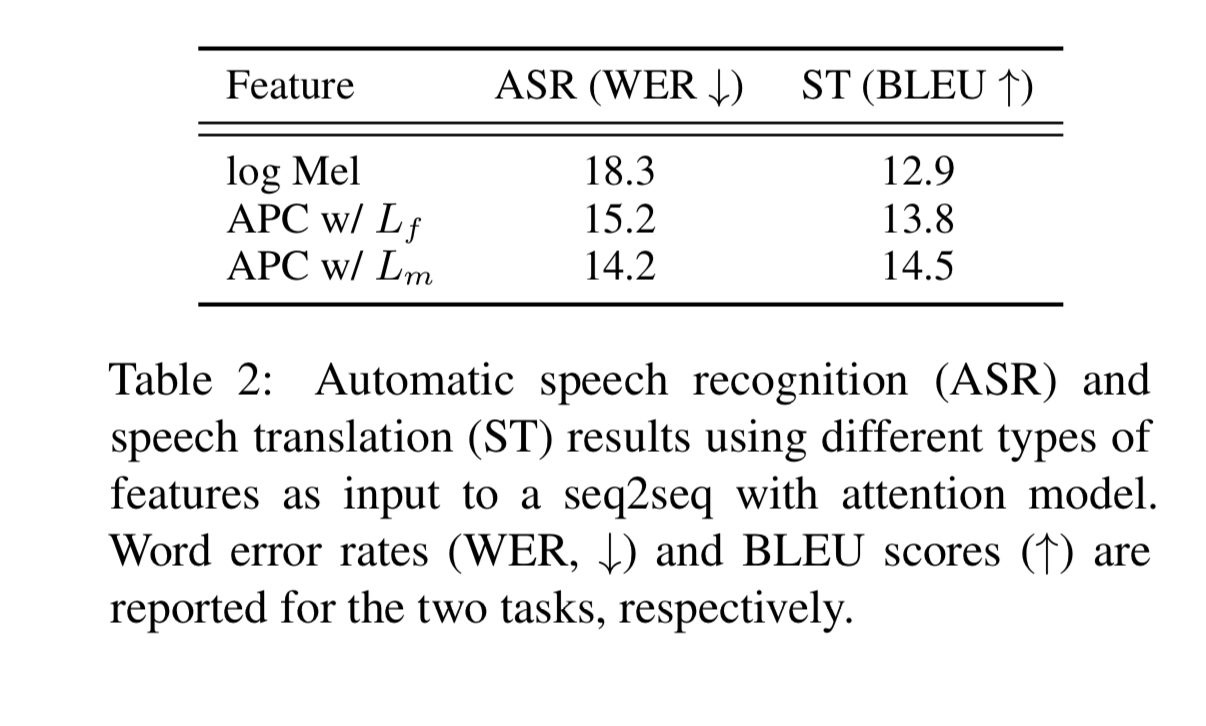
\includegraphics[width=0.5\textwidth]{APCexp}
%
%	{\footnotesize\color{softgrey} Table from \citep{chung2020improved}}
%\end{center}
%
%
%\end{frame}

\begin{frame}
\frametitle{Differences between speech and text SSL}
\begin{itemize}
\item Input speech representations (MFCCs for instance) are already in a vector form (no embedding layer)
\item More uncertainty 
 	\begin{itemize}
	\item text (discrete): finite number of possible outcomes (target tokens)
	\item speech and video (continuous): infinite number of frames that can plausibly follow a given audio (or video) clip
	\end{itemize}
\end{itemize} 
\begin{figure}
	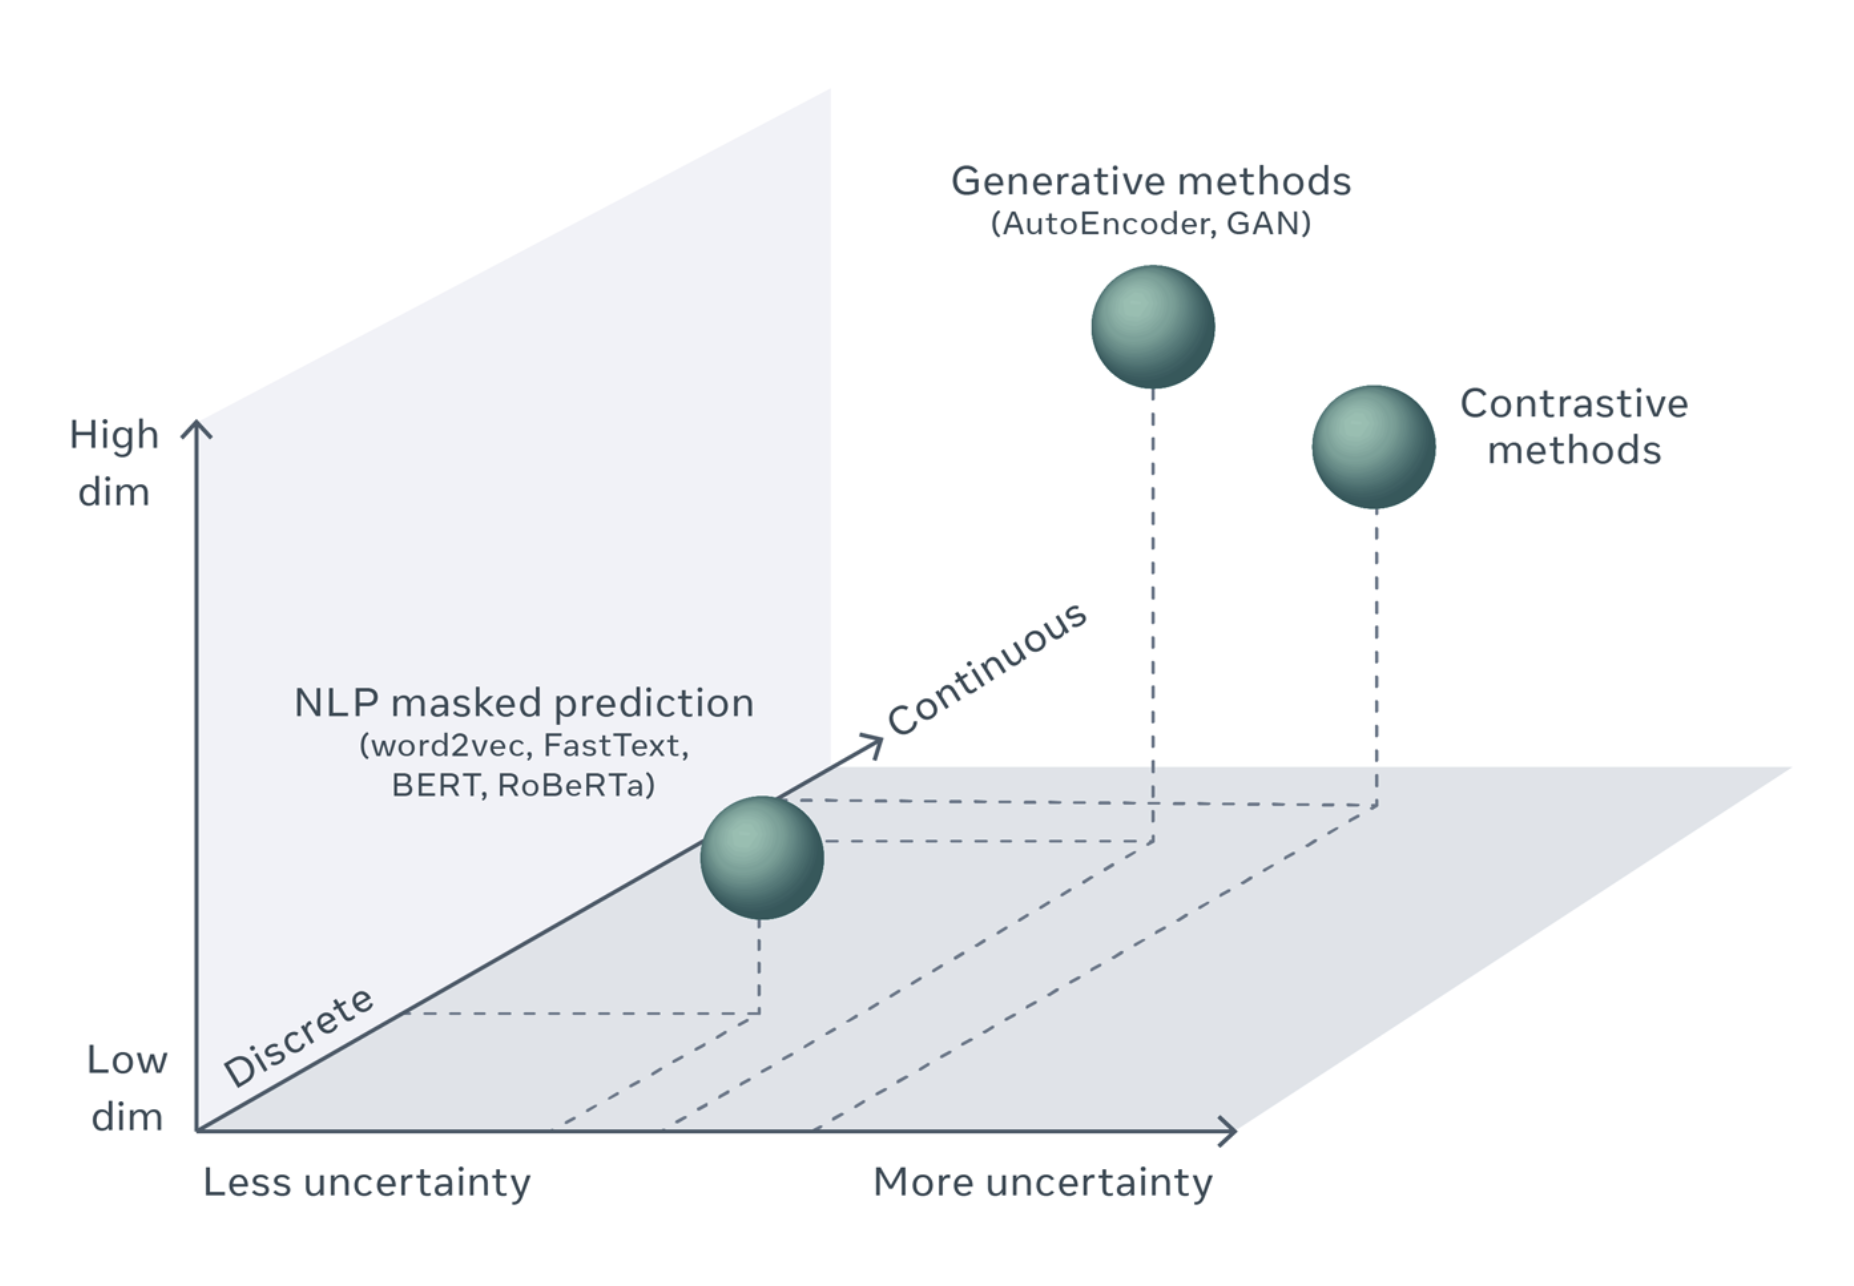
\includegraphics[width=0.4\textwidth]{lecunSSL}
	\caption{Figure from  \url{https://ai.facebook.com/blog/self-supervised-learning-the-dark-matter-of-intelligence}}
\end{figure}

\end{frame}

\begin{frame}
	\frametitle{Contrastive Predictive Coding (CPC)}
\begin{columns}[T]
\begin{column}{0.58\textwidth}
\small
		\begin{itemize}
			\item  Idea proposed by \cite{CPCfirstref}: maybe an easier objective (classification instead of regression)
			\item Contrastive loss: distinguish a true future sample $z_{i+k}$ from distractors drawn from the same utterance
			\item Example of \textit{wav2vec} \citep{DBLP:journals/corr/abs-1904-05862}, fully convolutional
			\begin{itemize}
				\item encoder $Z=f(X)$: $z_i$ encodes 30ms every 10ms
				\item context network $C=g(Z)$: $c_i$ sees 210ms
			\end{itemize}
			\item Learned representations improve a supervised ASR system
		\end{itemize} 
\end{column}
\begin{column}{0.4\textwidth}
		\begin{figure}
			\centering
			\vspace*{1.5em}
			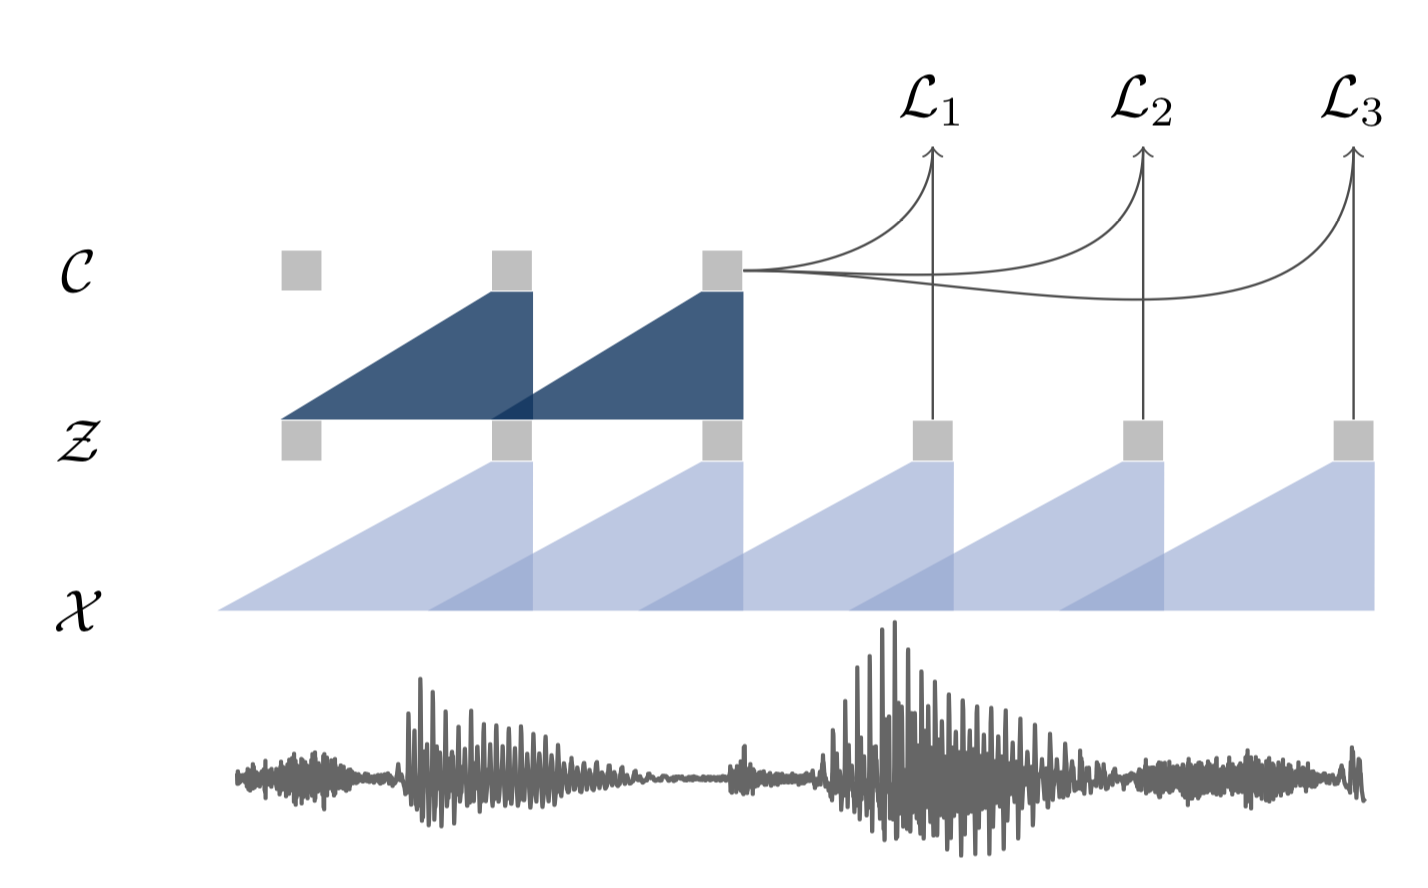
\includegraphics[width=\textwidth]	{unsupervisedspeech.png} 
			\caption{Figure from \citep{DBLP:journals/corr/abs-1904-05862}}
			\label{fig:unsup}
			\end{figure}
\end{column}
\end{columns}
\end{frame}


\begin{frame}
\frametitle{Follow-up approaches (2019-2020)}
		\begin{itemize}
			\item \textbf{Multiple self-supervised tasks}: PASE \citep{pascual2019} and PASE+ \citep{ravanelli2020multitask}
			\begin{itemize}
				\item one encoder, several ``workers'' reconstructing waveform, spectrum, MFCC, prosody + contrastive tasks
			\end{itemize}
			\item \textbf{Masked reconstruction of frames} (BERT-like, regression)
			\begin{itemize}
				\item Speech-XLNet \citep{song2019speechxlnet}, Mockingjay \citep{Liu_2020}, masking in time and frequency \citep{wang2020unsupervised}
			\end{itemize}
			\item Lessons learnt
			\begin{itemize}
				\item bidirectional Transformer encoders + masking work best
				\item predicting \textit{discrete} targets works better than regressing frames $\rightarrow$ wav2vec 2.0 and HuBERT
			\end{itemize}
		\end{itemize} 
\end{frame}


\begin{frame}
\frametitle{Wav2vec 2.0: masking + contrastive learning}

		\begin{itemize}
			\item Encode speech with CNN layers and then mask spans of the resulting latent speech representations (cf masked LM)
			\item Learn \textit{discrete} speech units as latent representations\footnote{Authors found this more effective than non-quantized targets}
			\item Latent representations fed to a Transformer network to build contextualized representations 
			\item Model trained with a contrastive task (true latent to be distinguished from distractors)
		\end{itemize}	
		
			\begin{figure}
			\centering
			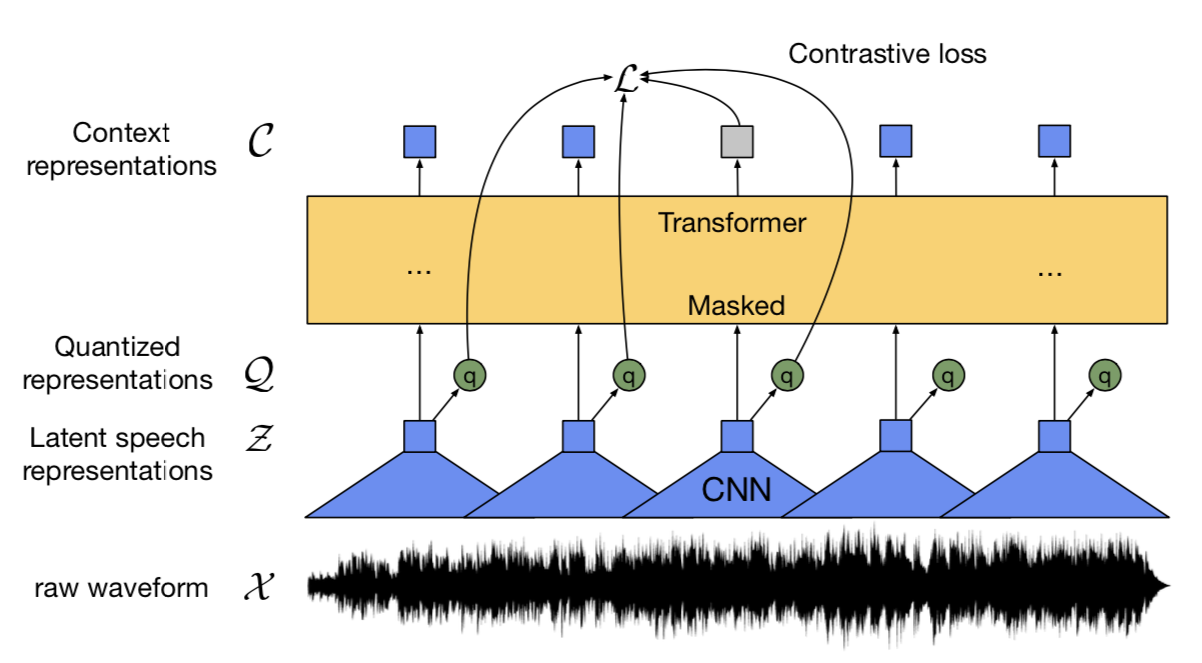
\includegraphics[scale=0.09]	{wav2vec2} 
		%	[scale=0.35,trim=0mm 140mm 0mm 0mm,clip=true]
			\caption{Figure from  \citep{DBLP:conf/nips/BaevskiZMA20}}
			\end{figure}

\end{frame}

\begin{frame}
\frametitle{Wav2vec 2.0: ASR with very few labels}
		\begin{itemize}
			\item Pre-train on unlabeled speech (53K hours, Libri-light), then fine-tune with CTC on a small labeled set \citep{DBLP:conf/nips/BaevskiZMA20}
		\end{itemize}
		\begin{center}
		\renewcommand{\arraystretch}{1.25}
		\begin{tabular}{lcc}
			\textbf{Labeled data} & \textbf{test-clean WER} & \textbf{test-other WER} \\
			\hline
			10 minutes & 4.8 & 8.2 \\
			960 hours (all Librispeech) & 1.8 & 3.3 \\
		\end{tabular}

		{\footnotesize\color{softgrey} Numbers from \citep{DBLP:conf/nips/BaevskiZMA20}}
		\end{center}
		\begin{itemize}
			\item With 1 hour of labels, beats the previous state of the art trained on 100 hours
			\item Multilingual versions: XLSR, then XLS-R (128 languages, 436K hours) \citep{babu2021xlsr}
			\item A game changer for low-resource languages
		\end{itemize}
\end{frame}


\begin{frame}
\frametitle{HuBERT: Hidden-Unit BERT}
\begin{columns}[T]
\begin{column}{0.55\textwidth}
\small
		\begin{itemize}
			\item Similar Conv+Transformer encoder \citep{DBLP:journals/corr/abs-2106-07447} but
			\item Cross-entropy loss (same as BERT) instead of contrastive loss
			\item Discrete targets built through a separate clustering process
			\item Learnt \textit{discrete} speech units refined at each iteration (3 iterations for large models)
			\item Matches or improves wav2vec 2.0 on Librispeech (10min to 960h of labels) ; X-Large (1B parameters): up to 13\% relative WER reduction on test-other
		\end{itemize}	
\end{column}
\begin{column}{0.43\textwidth}
			\begin{figure}
			\centering
			\vspace*{1em}
			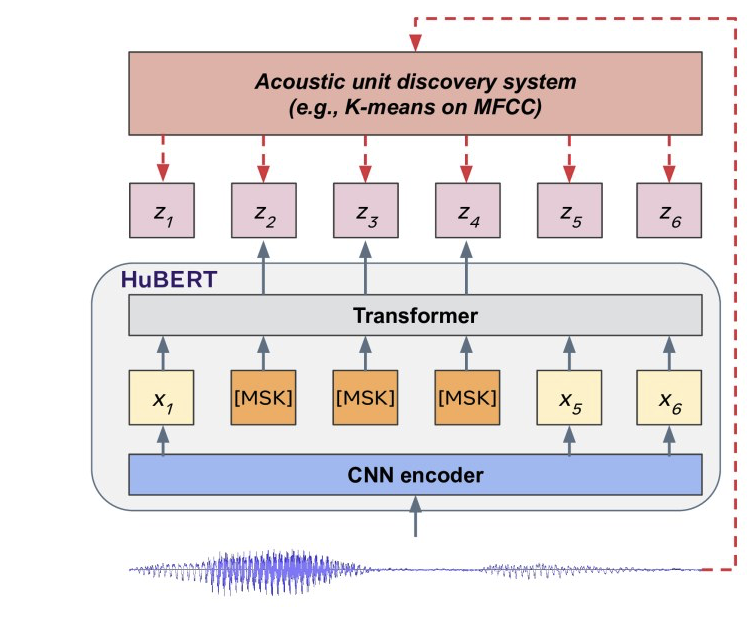
\includegraphics[width=\textwidth]	{hubert.png} 
			\caption{Figure from  \citep{DBLP:journals/corr/abs-2106-07447}}
			\end{figure}
\end{column}
\end{columns}
\end{frame}

\begin{frame}
\frametitle{HuBERT: where do the targets come from?}
\begin{center}
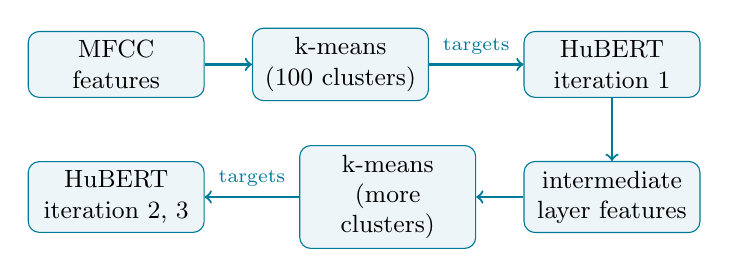
\begin{tikzpicture}[every node/.style={font=\small},
  box/.style={draw=accent, rounded corners, fill=blockbg, minimum height=0.8cm, align=center, text width=2.0cm},
  arr/.style={->, thick, accent}]
  \node[box] (mfcc) {MFCC features};
  \node[box, right=0.6cm of mfcc] (km1) {k-means\\(100 clusters)};
  \node[box, right=1.2cm of km1] (it1) {HuBERT\\iteration 1};
  \node[box, below=0.8cm of it1] (feat) {intermediate layer features};
  \node[box, left=0.6cm of feat] (km2) {k-means\\(more clusters)};
  \node[box, left=1.2cm of km2] (it2) {HuBERT\\iteration 2, 3};
  \draw[arr] (mfcc) -- (km1);
  \draw[arr] (km1) -- node[above, font=\scriptsize]{targets} (it1);
  \draw[arr] (it1) -- (feat);
  \draw[arr] (feat) -- (km2);
  \draw[arr] (km2) -- node[above, font=\scriptsize]{targets} (it2);
\end{tikzpicture}

{\tiny After \citep{DBLP:journals/corr/abs-2106-07447}}
\end{center}
\begin{itemize}
	\item Loss computed on masked frames only: the model must learn an acoustic \textit{and} a language model of the units
	\item Works because the clustering is \textit{consistent}, not because clusters are good phones
	\item These cluster indices are \textbf{discrete speech units}: the first ``speech tokens'' (see next section)
\end{itemize}
\end{frame}


\begin{frame}
\frametitle{After HuBERT}
		\begin{itemize}
			\item \textbf{WavLM} \citep{chen2022wavlm}
			\begin{itemize}
				\item masked prediction (like HuBERT) + denoising: the input is mixed with noise or another speaker
				\item good for ASR \textit{and} speaker, diarization, separation tasks (``full stack'')
			\end{itemize}
			\item \textbf{w2v-BERT} \citep{chung2021w2vbert}
			\begin{itemize}
				\item contrastive learning (wav2vec 2.0) + masked prediction (BERT), trained end-to-end, no re-clustering
			\end{itemize}
			\item \textbf{data2vec} \citep{baevski2022data2vec}
			\begin{itemize}
				\item predict the teacher's \textit{contextualized} representations of the unmasked input (self-distillation)
				\item same method for speech, vision and text
			\end{itemize}
			\item Multilingual: XLS-R \citep{babu2021xlsr}, mHuBERT-147 \citep{zanonboito2024mhubert}
			\item Today SSL encoders are the front-end of most ASR systems and speech LLMs
		\end{itemize} 
\end{frame}


% --- SUPERB slide commented out (uncomment to restore) ---
%\begin{frame}
%\frametitle{Evaluating SSL models: SUPERB}
%\small
%		\begin{itemize}
%			\item SUPERB \citep{yang_superb_2021}: SSL encoder \textit{frozen}, learnable weighted sum of its layers, small task-specific heads
%			\item Tasks: content (PR, ASR, KS), speaker (SID, ASV, SD), semantics (IC, SF), paralinguistics (ER)
%			\item ML-SUPERB \citep{shi2023mlsuperb}: 143 languages (ASR + language ID)
%		\end{itemize}
%		\vspace*{-0.5em}
%		\begin{figure}
%			\centering
%			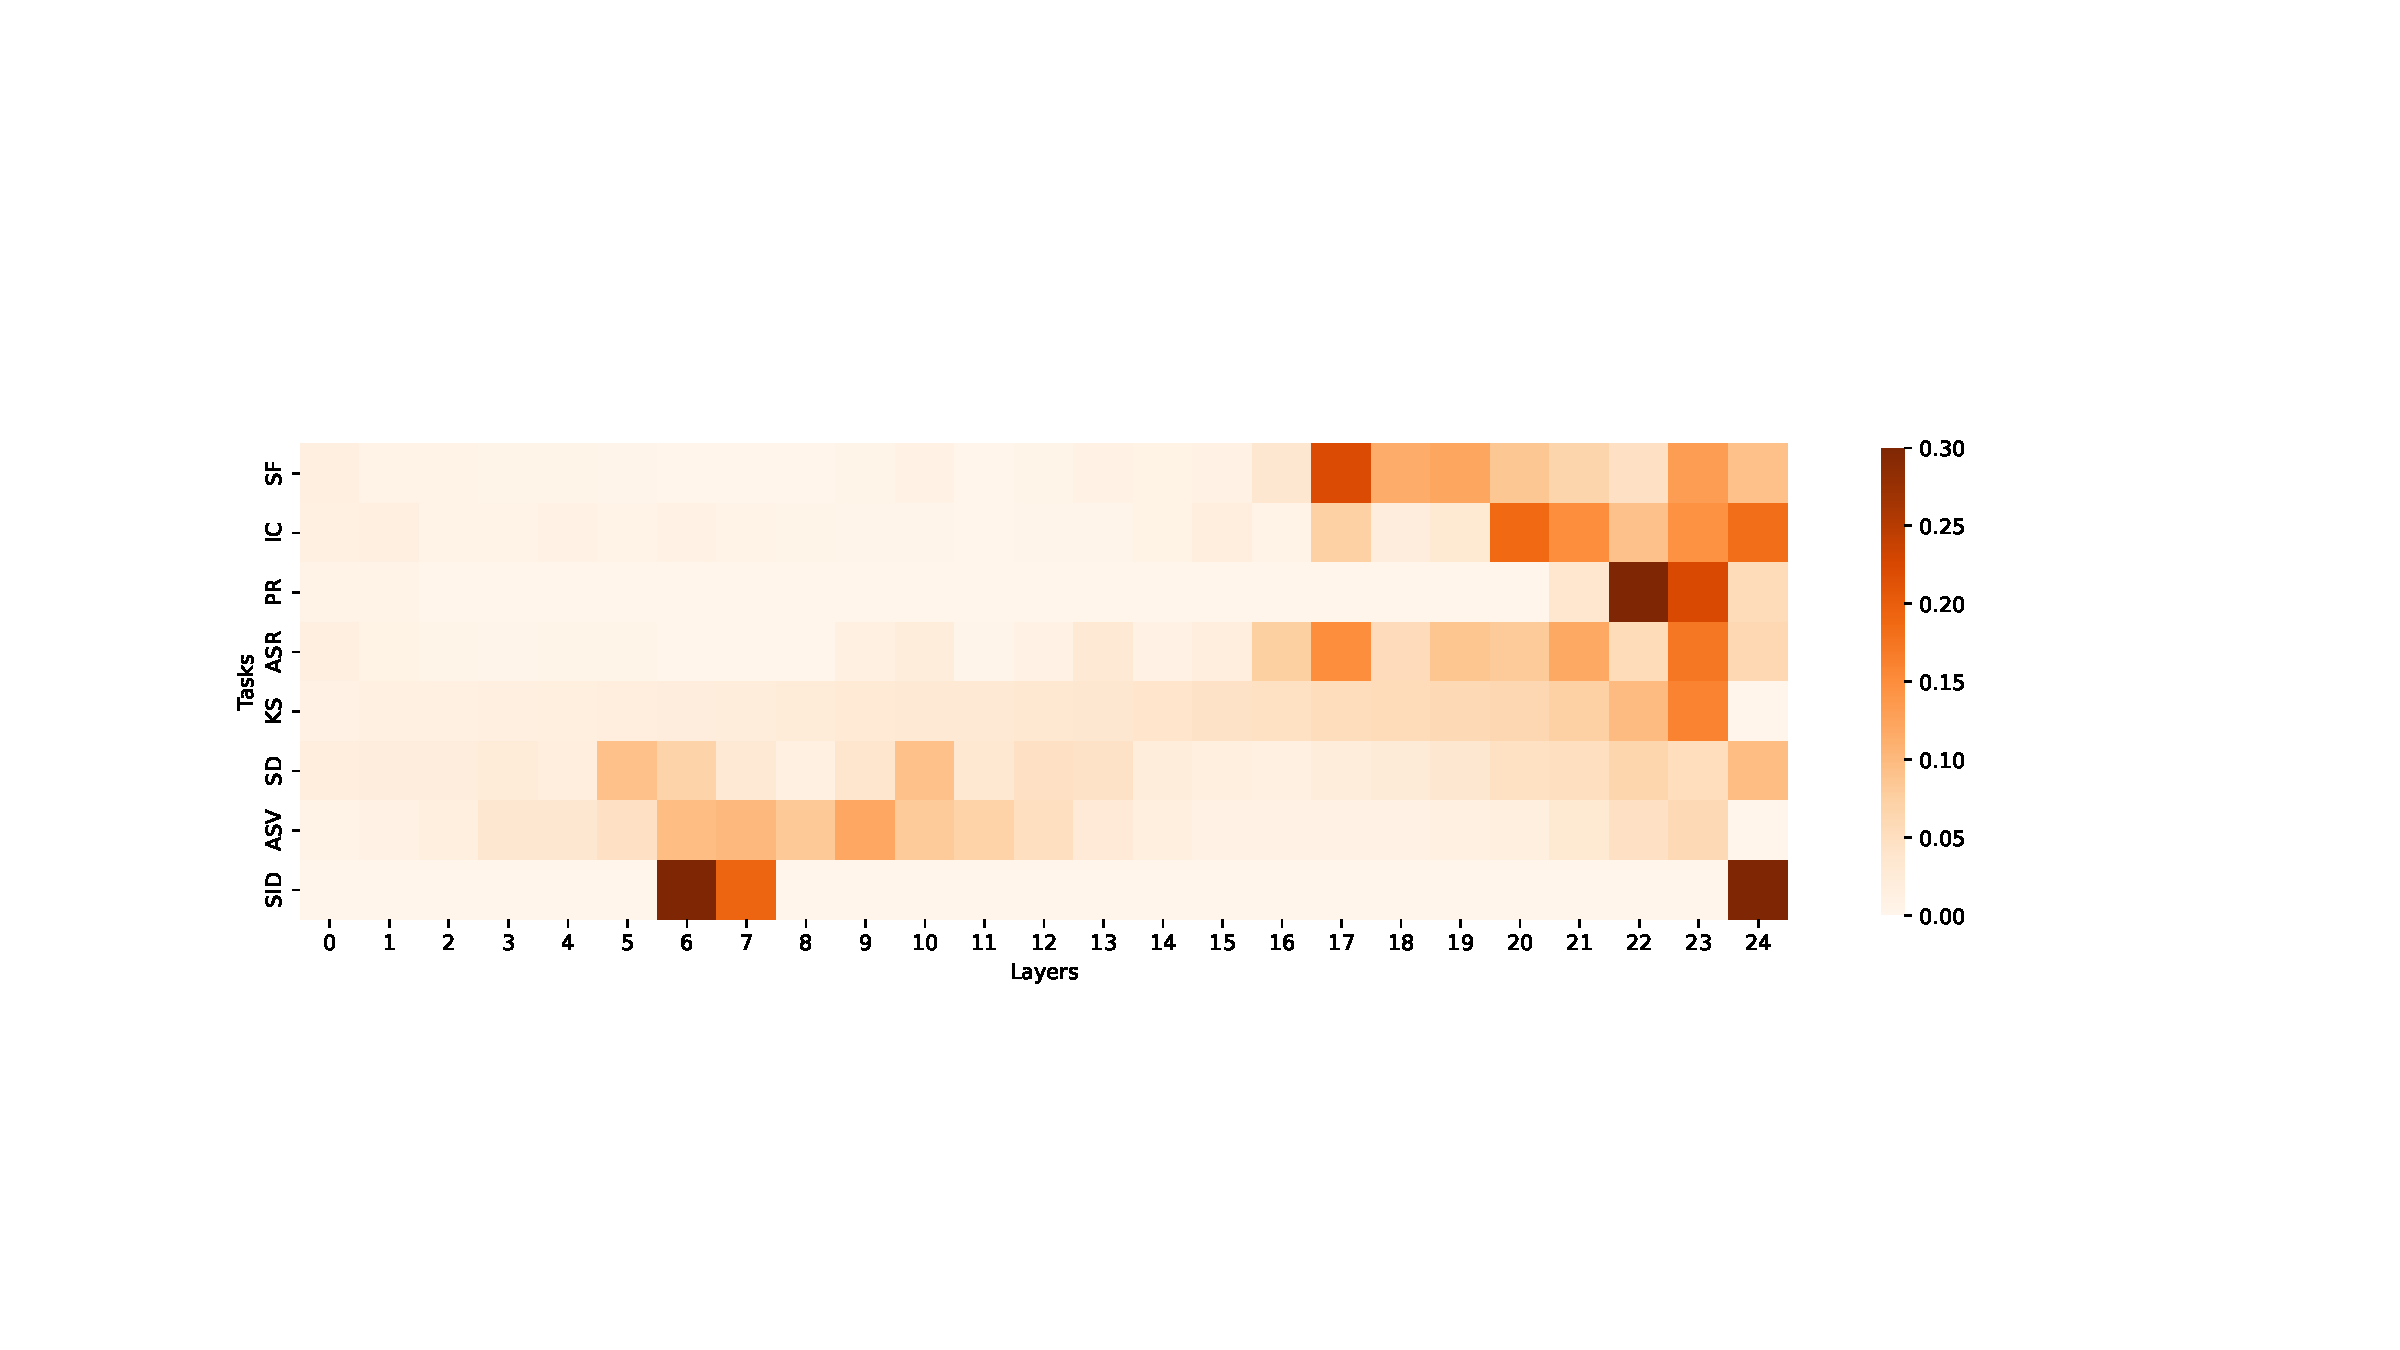
\includegraphics[width=0.92\textwidth, trim=100 160 200 200, clip]{images2026/wavlm-superb-layer-weights.pdf}
%			\caption{Learnt layer weights of WavLM Large per SUPERB task: speaker tasks use lower layers, content and semantics use upper layers. Figure from \citep{chen2022wavlm}}
%		\end{figure}
%\end{frame}


%_______________________________________________________

\section{Speech as tokens}

\frame{\tableofcontents[currentsection]}

\begin{frame}
\frametitle{Why turn speech into tokens?}
\begin{itemize}
	\item LLMs work on \textit{discrete} tokens ; speech is a continuous signal
	\item Speech units allow LMs trained on audio only (\textit{textless} NLP, e.g. GSLM \citep{lakhotia2021gslm} on HuBERT units)
	\item But speech is much \textit{longer} than text
\end{itemize}
\begin{center}
\renewcommand{\arraystretch}{1.2}
\small
\begin{tabular}{lr}
	\textbf{Representation} & \textbf{Tokens per second} \\
	\hline
	Text (English, subwords) & $\approx$ 3--4 \\
	Waveform (16kHz samples) & 16,000 \\
	HuBERT units (20ms frames) & 50 \\
	EnCodec, 6kbps (75Hz $\times$ 8 codebooks) & 600 \\
	Mimi (12.5Hz $\times$ 8 codebooks) & 100 \\
\end{tabular}

{\footnotesize\color{softgrey} Codec rates from \citep{defossez2022encodec,moshi2024}}
\end{center}
\begin{itemize}
	\item Goal: few tokens/s, keeping \textit{what} is said and \textit{how}
\end{itemize}
\end{frame}


\begin{frame}
\frametitle{Semantic vs. acoustic tokens}
\begin{columns}[T]
\begin{column}{0.48\textwidth}
\small
\begin{itemize}
	\item \textbf{Semantic tokens}: k-means on SSL features (HuBERT, w2v-BERT)
	\begin{itemize}
		\item phonetic content, long-term structure
		\item lose speaker and prosody
	\end{itemize}
	\item \textbf{Acoustic tokens}: neural audio codec
	\begin{itemize}
		\item high-quality waveform reconstruction
		\item little linguistic structure
	\end{itemize}
	\item AudioLM \citep{borsos2022audiolm}: semantic tokens first, then acoustic tokens
\end{itemize}
\end{column}
\begin{column}{0.5\textwidth}
\begin{figure}
	\centering
	\vspace*{1.5em}
	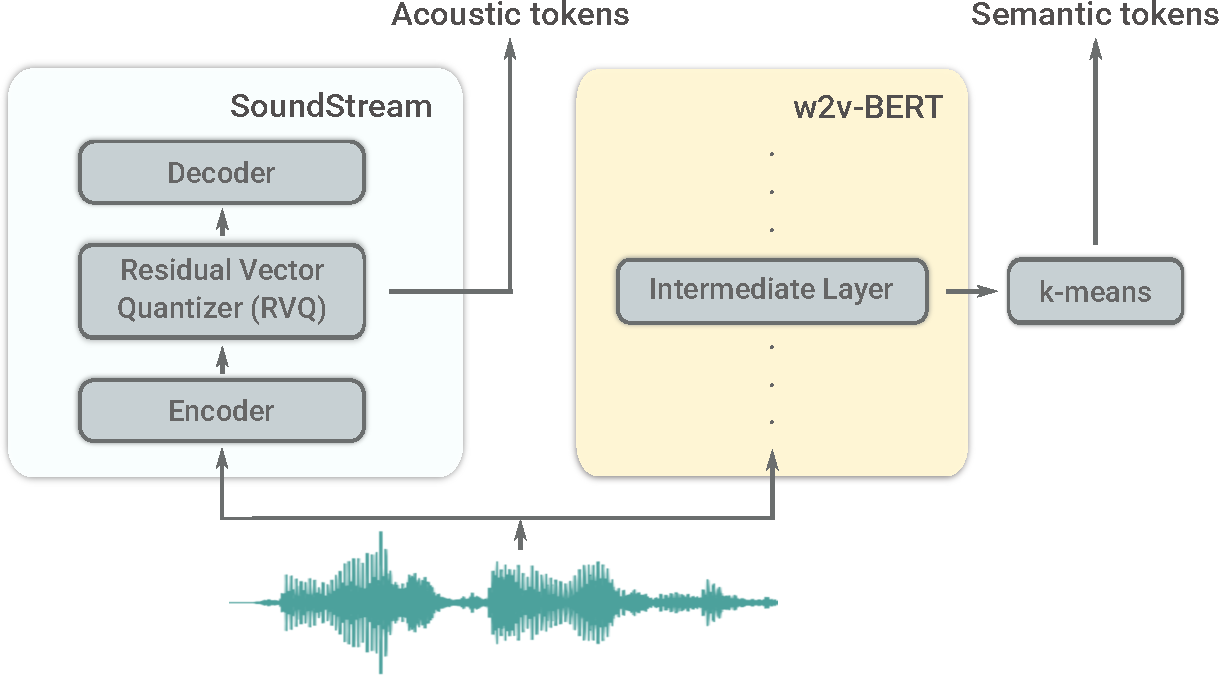
\includegraphics[width=\textwidth]{images2026/audiolm-tokenizers.pdf}
	\caption{Figure from \citep{borsos2022audiolm}}
\end{figure}
\end{column}
\end{columns}
\end{frame}


\begin{frame}
\frametitle{Neural audio codecs and RVQ}
\small
\begin{itemize}
	\item Convolutional encoder $\rightarrow$ quantizer $\rightarrow$ decoder, trained end-to-end with reconstruction + adversarial losses: SoundStream \citep{zeghidour2021soundstream}, EnCodec \citep{defossez2022encodec}
	\item \textbf{Residual vector quantization (RVQ)}: codebook 1 quantizes the encoder output, codebook 2 quantizes what is left (the residual), etc.
	\begin{itemize}
		\item first codebooks: coarse information ; last ones: fine details
		\item bitrate = frame rate $\times$ \#codebooks $\times \log_2$(codebook size)
		\item fewer codebooks = lower bitrate (SoundStream: 3 to 18 kbps)
	\end{itemize}
\end{itemize}
\begin{figure}
	\centering
	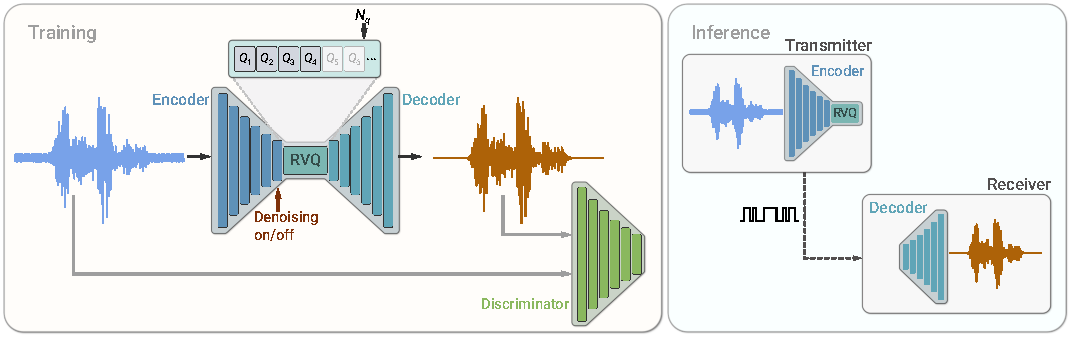
\includegraphics[height=2.5cm]{images2026/soundstream-architecture.pdf}
	\vspace*{-0.6em}
	\caption{Figure from \citep{zeghidour2021soundstream}}
\end{figure}
\end{frame}


\begin{frame}
\frametitle{Mimi: semantic and acoustic tokens in one codec}
\small
\begin{itemize}
	\item SpeechTokenizer \citep{zhang2023speechtokenizer}: the first RVQ level is distilled from HuBERT, so it carries the semantics
	\item Mimi \citep{moshi2024}, the codec of Moshi
	\begin{itemize}
		\item 24kHz audio $\rightarrow$ 12.5 frames/s, 8 codebooks, 1.1 kbps
		\item first codebook distilled from WavLM (semantic), 7 others acoustic
		\item causal (streaming) encoder and decoder, with Transformers
	\end{itemize}
\end{itemize}
\begin{figure}
	\centering
	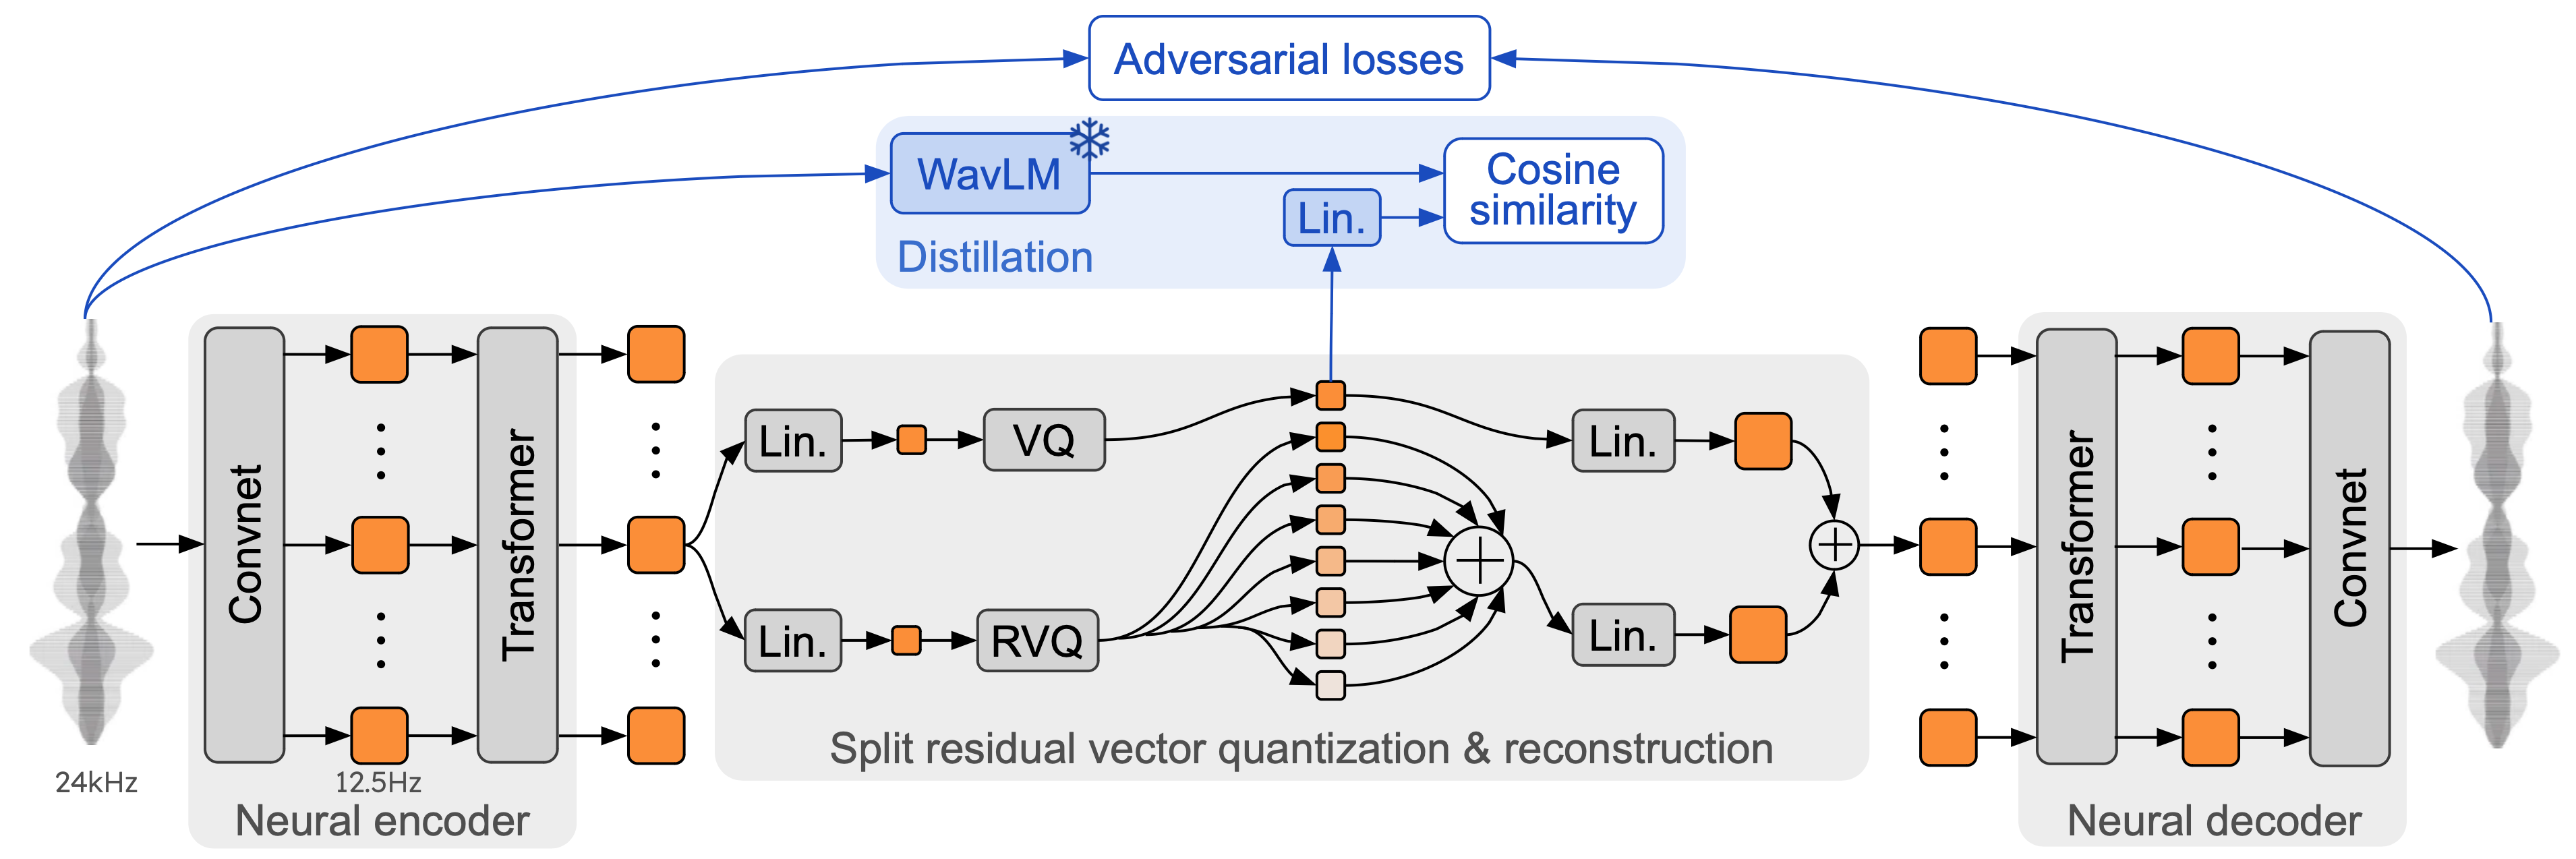
\includegraphics[width=0.86\textwidth]{images2026/mimi-architecture.png}
	\caption{Figure from \citep{moshi2024}}
\end{figure}
\end{frame}

%_______________________________________________________

\quizbreak{3}{3}

\section{When LLMs learn to listen}

\frame{\tableofcontents[currentsection]}

\begin{frame}
\frametitle{SpeechT5 \citep{SpeechT5}}
\begin{columns}[T]
  \begin{column}{0.4\textwidth}
  \small
    \begin{itemize}
        \item Multimodal extension of encoder-decoder models such as T5
        \item One Transformer backbone for speech \textit{and} text, with modality-specific pre/post-nets
        \item Shared vector space for acoustic and text information
        \item Initializes ASR, TTS, voice conversion, speaker id., etc.
    \end{itemize}
  \end{column}
  \begin{column}{0.6\textwidth}
    \begin{figure}
        \centering
        \vspace*{1em}
        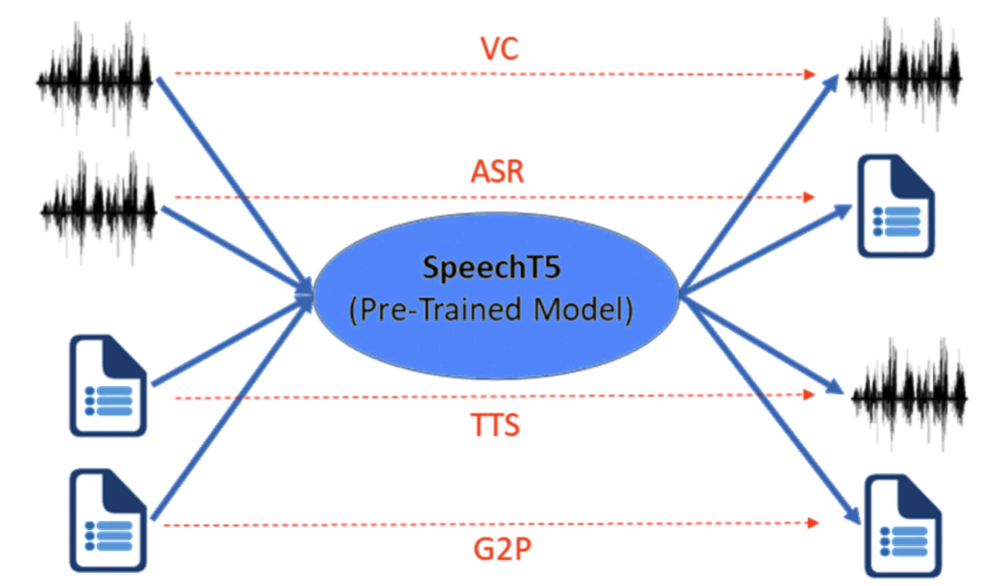
\includegraphics[width=\textwidth]{images/speechT5.png}
        \caption{Figure from \citep{SpeechT5}}
    \end{figure}
  \end{column}
\end{columns}
\end{frame}

\begin{frame}
\frametitle{SpeechT5: pre-training and results}
\small
\begin{itemize}
    \item Composite pre-training loss: masked prediction of discrete speech units (\textit{à la} HuBERT), speech reconstruction (filterbanks), text denoising (\textit{à la} BART), cross-modal alignment
    \item Slightly better than speech-only pre-training on ASR, TTS, voice conversion, speaker id.
\end{itemize}
\begin{figure}
    \centering
    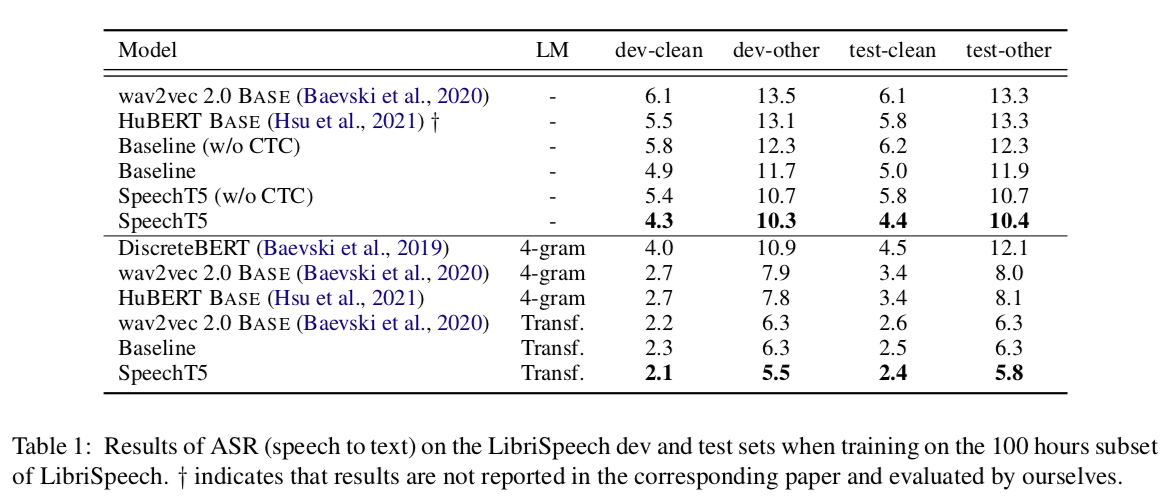
\includegraphics[width=0.95\textwidth]{images/ASRspeecht5.png}
    \vspace*{-0.8em}
    \caption{Table from \citep{SpeechT5}}
\end{figure}
\end{frame}


\begin{frame}
\frametitle{Two ways to connect speech to an LLM}
\begin{center}
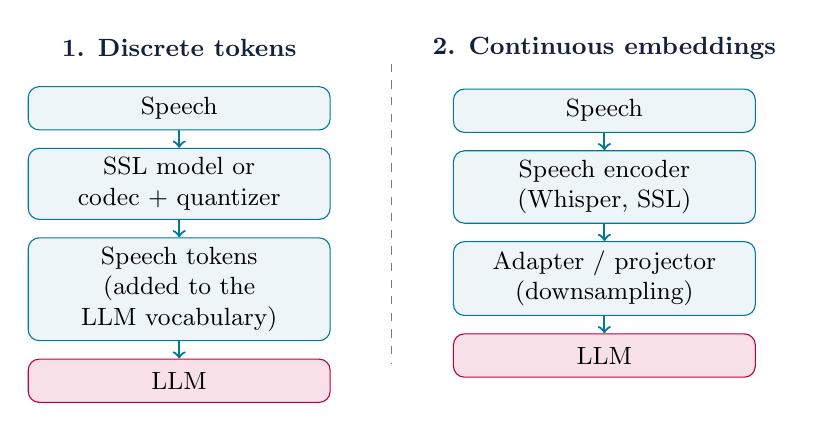
\begin{tikzpicture}[every node/.style={font=\small},
  box/.style={draw=accent, rounded corners, fill=blockbg, minimum height=0.55cm, align=center, text width=3.6cm},
  llm/.style={draw=purple, rounded corners, fill=purple!12, minimum height=0.55cm, align=center, text width=3.6cm},
  arr/.style={->, thick, accent}]
  \node[font=\small\bfseries, text=titleink] (t1) at (0,0) {1. Discrete tokens};
  \node[box, below=0.25cm of t1] (s1) {Speech};
  \node[box, below=0.22cm of s1] (q1) {SSL model or codec + quantizer};
  \node[box, below=0.22cm of q1] (u1) {Speech tokens\\(added to the LLM vocabulary)};
  \node[llm, below=0.22cm of u1] (l1) {LLM};
  \draw[arr] (s1) -- (q1); \draw[arr] (q1) -- (u1); \draw[arr] (u1) -- (l1);
  \node[font=\small\bfseries, text=titleink] (t2) at (5.4,0) {2. Continuous embeddings};
  \node[box, below=0.25cm of t2] (s2) {Speech};
  \node[box, below=0.22cm of s2] (e2) {Speech encoder\\(Whisper, SSL)};
  \node[box, below=0.22cm of e2] (a2) {Adapter / projector\\(downsampling)};
  \node[llm, below=0.22cm of a2] (l2) {LLM};
  \draw[arr] (s2) -- (e2); \draw[arr] (e2) -- (a2); \draw[arr] (a2) -- (l2);
  \draw[dashed, softgrey] (2.7,-0.2) -- (2.7,-4.0);
\end{tikzpicture}
\end{center}
\vspace*{-0.8em}
\begin{columns}[T]
\begin{column}{0.48\textwidth}
\scriptsize
\begin{itemize}
	\item[{\color{LigAikumaGreen}+}] speech in \textit{and} out, same LM loss (SpeechGPT \citep{zhang2023speechgpt}, Moshi)
	\item[{\color{red}--}] long sequences, may lose acoustic detail
\end{itemize}
\end{column}
\begin{column}{0.48\textwidth}
\scriptsize
\begin{itemize}
	\item[{\color{LigAikumaGreen}+}] keeps acoustic detail, reuses strong encoders
	\item[{\color{red}--}] speech in, text out (needs a separate speech generator)
\end{itemize}
\end{column}
\end{columns}
\end{frame}


\begin{frame}
\frametitle{The standard recipe: encoder + adapter + LLM}
\small
\begin{itemize}
	\item Pre-trained speech encoder, often frozen (e.g. Whisper)
	\item Adapter (can be a simple MLP or more complex) reduces the frame rate and maps to the LLM embedding space
	\item Text LLM, frozen or with LoRA
	\item Training: alignment (ASR, captioning), then instruction tuning
	\item SALMONN \citep{tang2023salmonn}, Qwen-Audio \citep{chu2023qwenaudio,chu2024qwen2audio}, Voxtral \citep{liu2025voxtral}
\end{itemize}
\begin{figure}
	\centering
	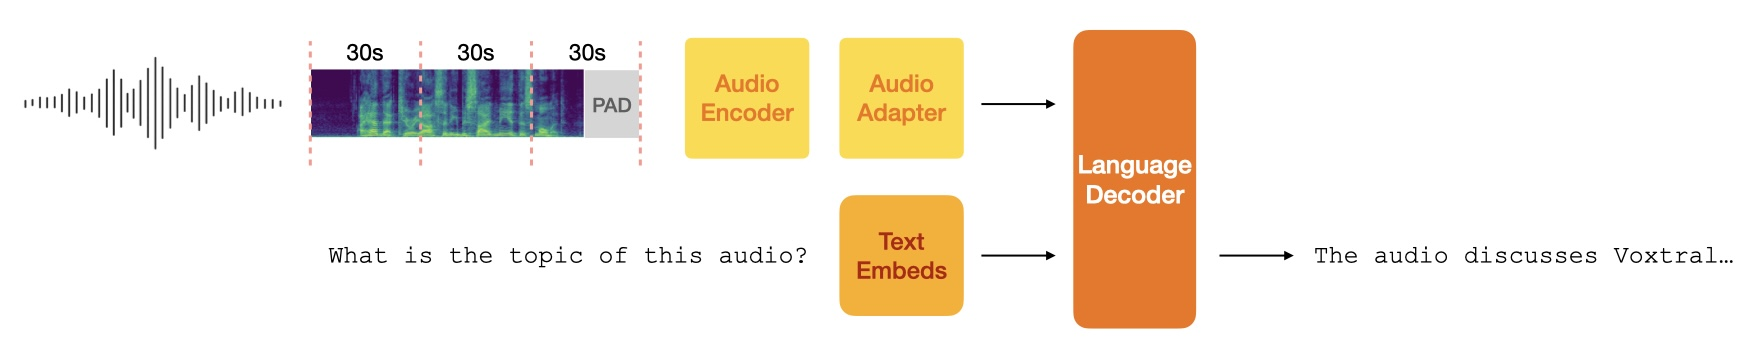
\includegraphics[width=\textwidth]{images2026/voxtral-architecture.jpeg}
	\caption{Voxtral: Whisper encoder, MLP adapter (50Hz $\rightarrow$ 12.5Hz), LLM decoder. Figure from \citep{liu2025voxtral}}
\end{figure}
\end{frame}


\begin{frame}
\frametitle{LLM-based ASR}
\begin{columns}[T]
\begin{column}{0.58\textwidth}
\small
\begin{itemize}
	\item Audio embeddings prepended to the text of a decoder-only LLM (Speech-LLaMA \citep{wu2023decoderonlyarchitecturespeechtotextlarge})
	\item In-context learning \citep{chen2023salmspeechaugmentedlanguagemodel}: e.g. new languages from a few examples \citep{omnilingual2025}
	\item Best WERs on the Open ASR Leaderboard (Canary-Qwen, Granite Speech, Qwen3-ASR)
	\item[{\color{LigAikumaGreen}+}] prompts and context (names, domain), LLM knowledge
	\item[{\color{red}--}] slower (autoregressive), and \textbf{hallucinations}
\end{itemize}
\end{column}
\begin{column}{0.4\textwidth}
\begin{figure}
	\centering
	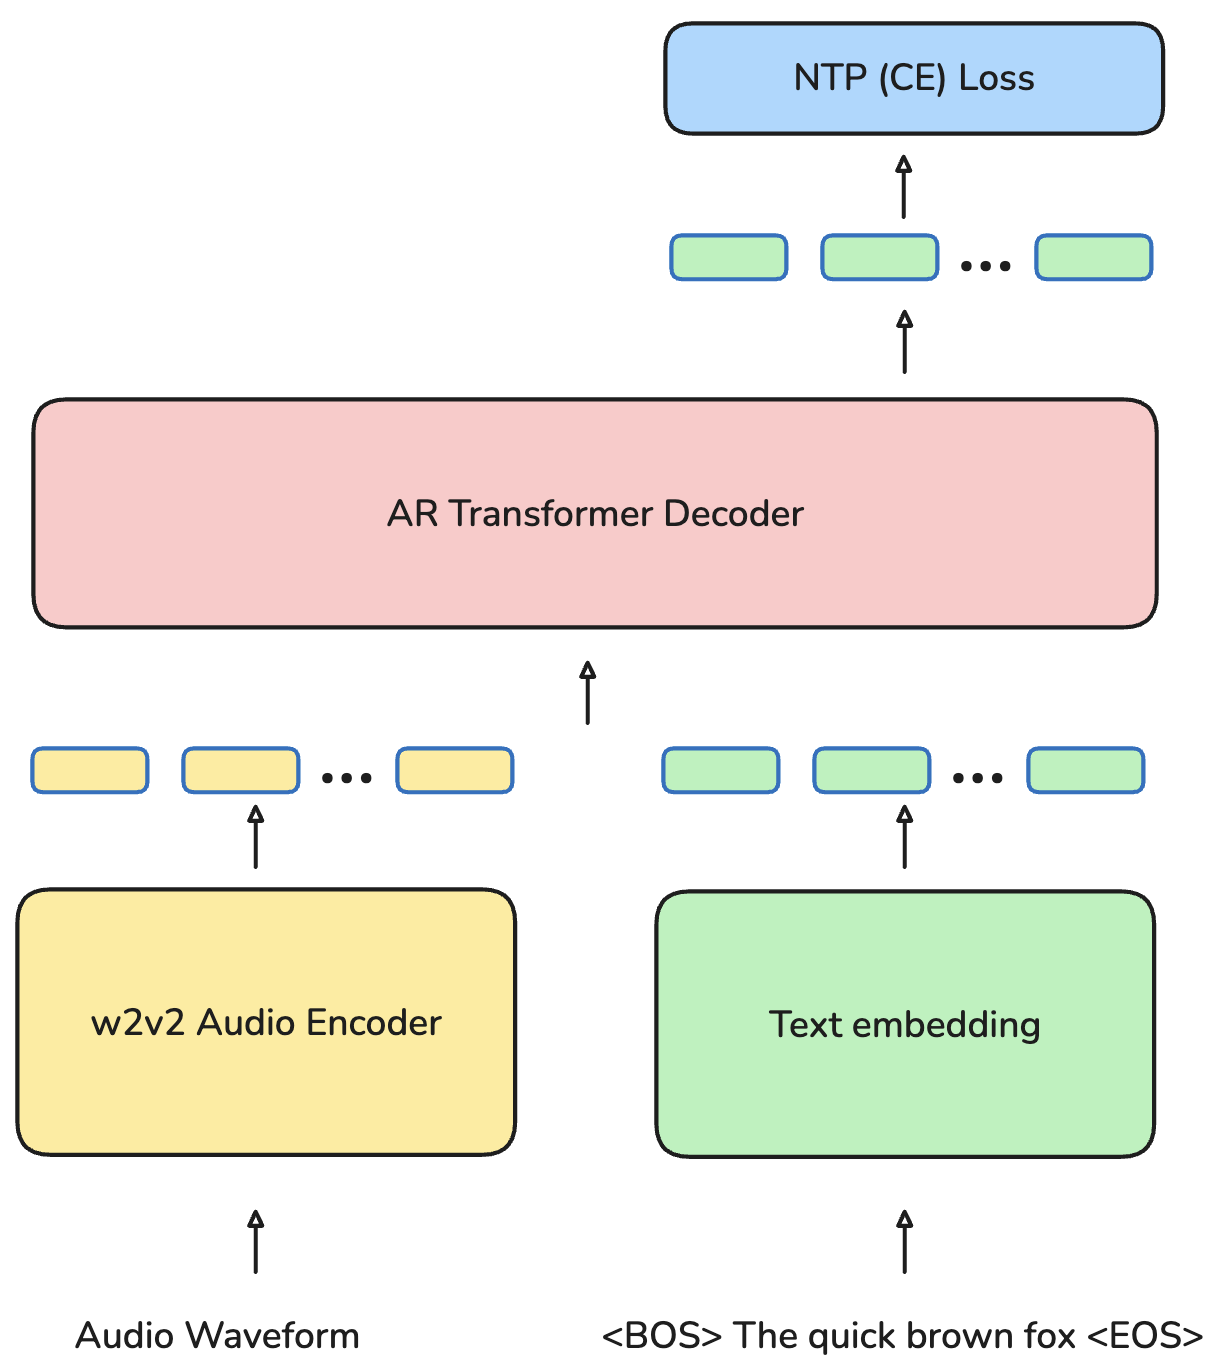
\includegraphics[width=0.9\textwidth]{images2026/omnilingual-llm-asr.png}
	\caption{LLM-ASR in Omnilingual ASR. Figure from \citep{omnilingual2025}}
\end{figure}
\end{column}
\end{columns}
\end{frame}


\begin{frame}
\frametitle{Omni models: speech in, speech out}
\begin{columns}[T]
\begin{column}{0.48\textwidth}
\small
\begin{itemize}
	\item GPT-4o \citep{openai2024gpt4o}: one network for text, audio, image ; answers in 320ms on average (like humans)
	\item Qwen2.5-Omni \citep{xu2025qwen25omni}: \textbf{Thinker} (LLM, generates text) + \textbf{Talker} (generates speech tokens, streaming)
	\item Qwen3-Omni \citep{xu2025qwen3omni}: Thinker-Talker with mixture of experts
	\item Still \textbf{turn-based}: waits for the user to finish $\rightarrow$ next section
\end{itemize}
\end{column}
\begin{column}{0.5\textwidth}
\begin{figure}
	\centering
	\vspace*{1em}
	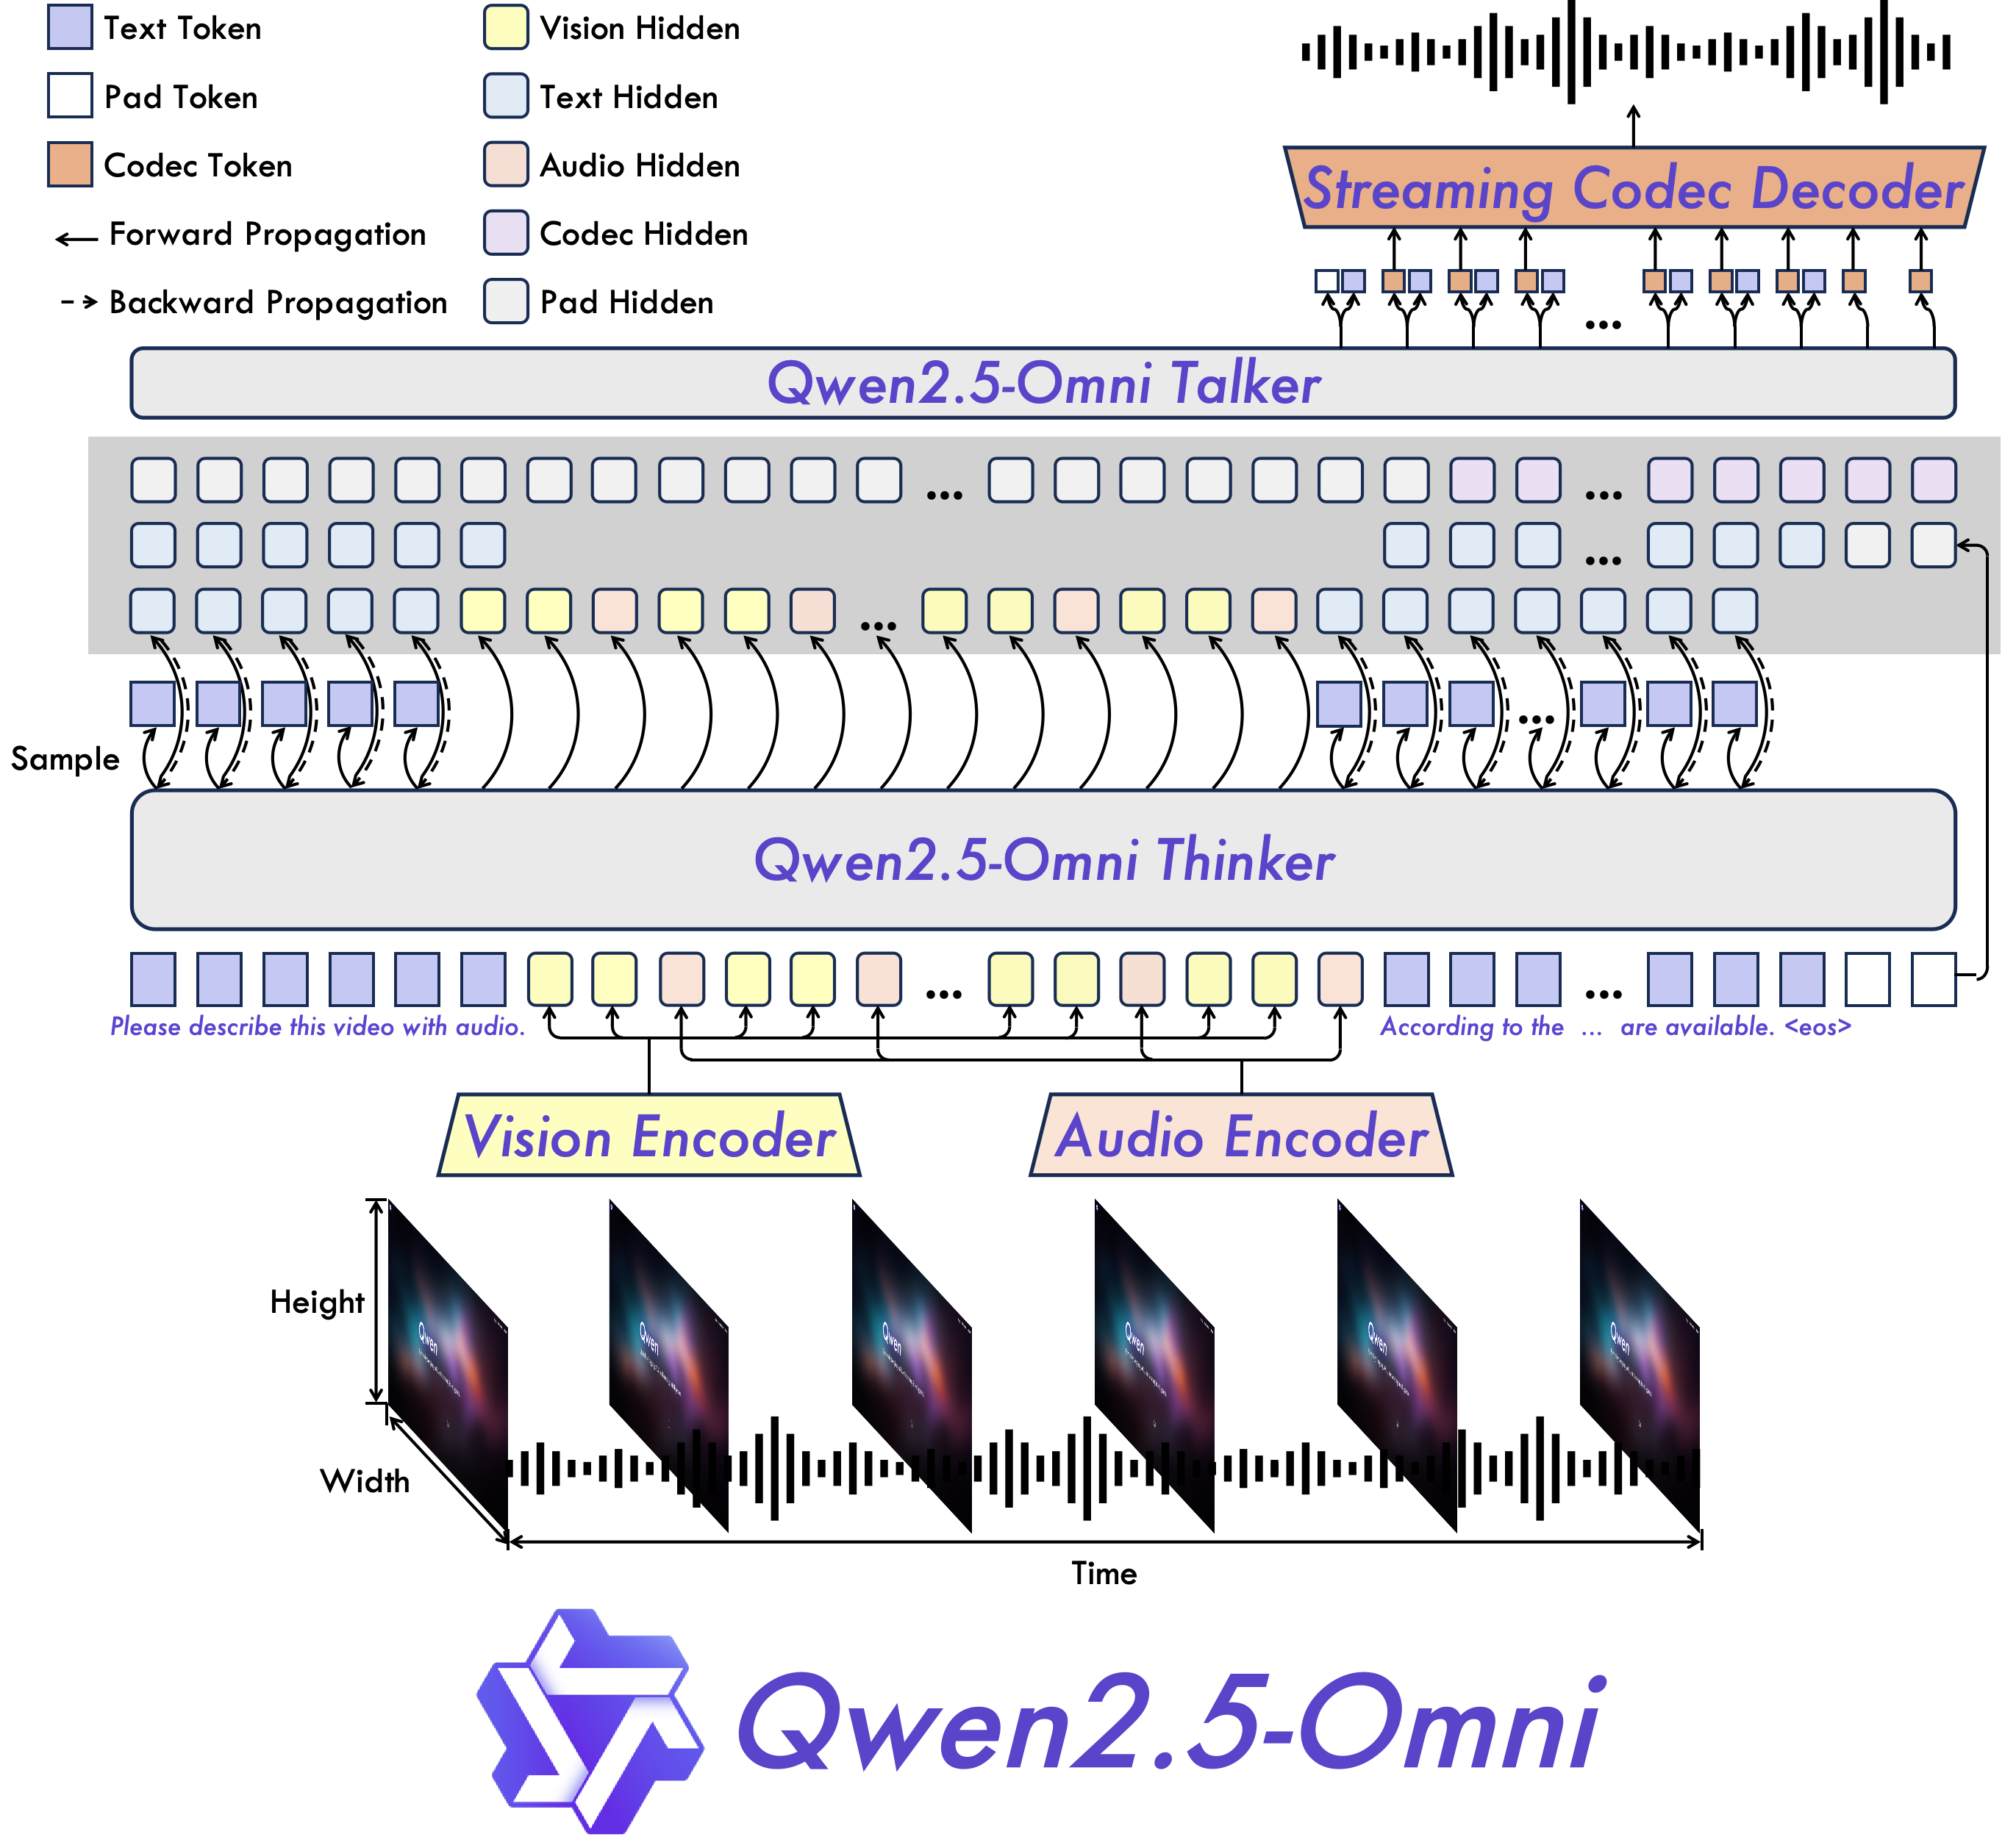
\includegraphics[width=\textwidth, trim=0 430 0 0, clip]{images2026/qwen25omni-thinker-talker.png}
	\caption{Figure from \citep{xu2025qwen25omni}}
\end{figure}
\end{column}
\end{columns}
\end{frame}


\begin{frame}
\frametitle{Hallucinations: when WER is not enough}
\small
\begin{itemize}
	\item Whisper (API, 2023): $\approx$1\% of transcriptions contain entire hallucinated phrases, 38\% of them harmful \citep{koenecke2024careless}
	\item More frequent for speakers with aphasia (1.7\% vs. 1.2\%), linked to longer non-vocal segments
	\item Autoregressive decoders can \textit{invent} fluent text during pauses or non-speech audio
	\item WER counts it like any insertion $\rightarrow$ report hallucinations separately
	\item Mitigations: voice activity detection, CTC or joint decoding
\end{itemize}
\begin{figure}
	\centering
	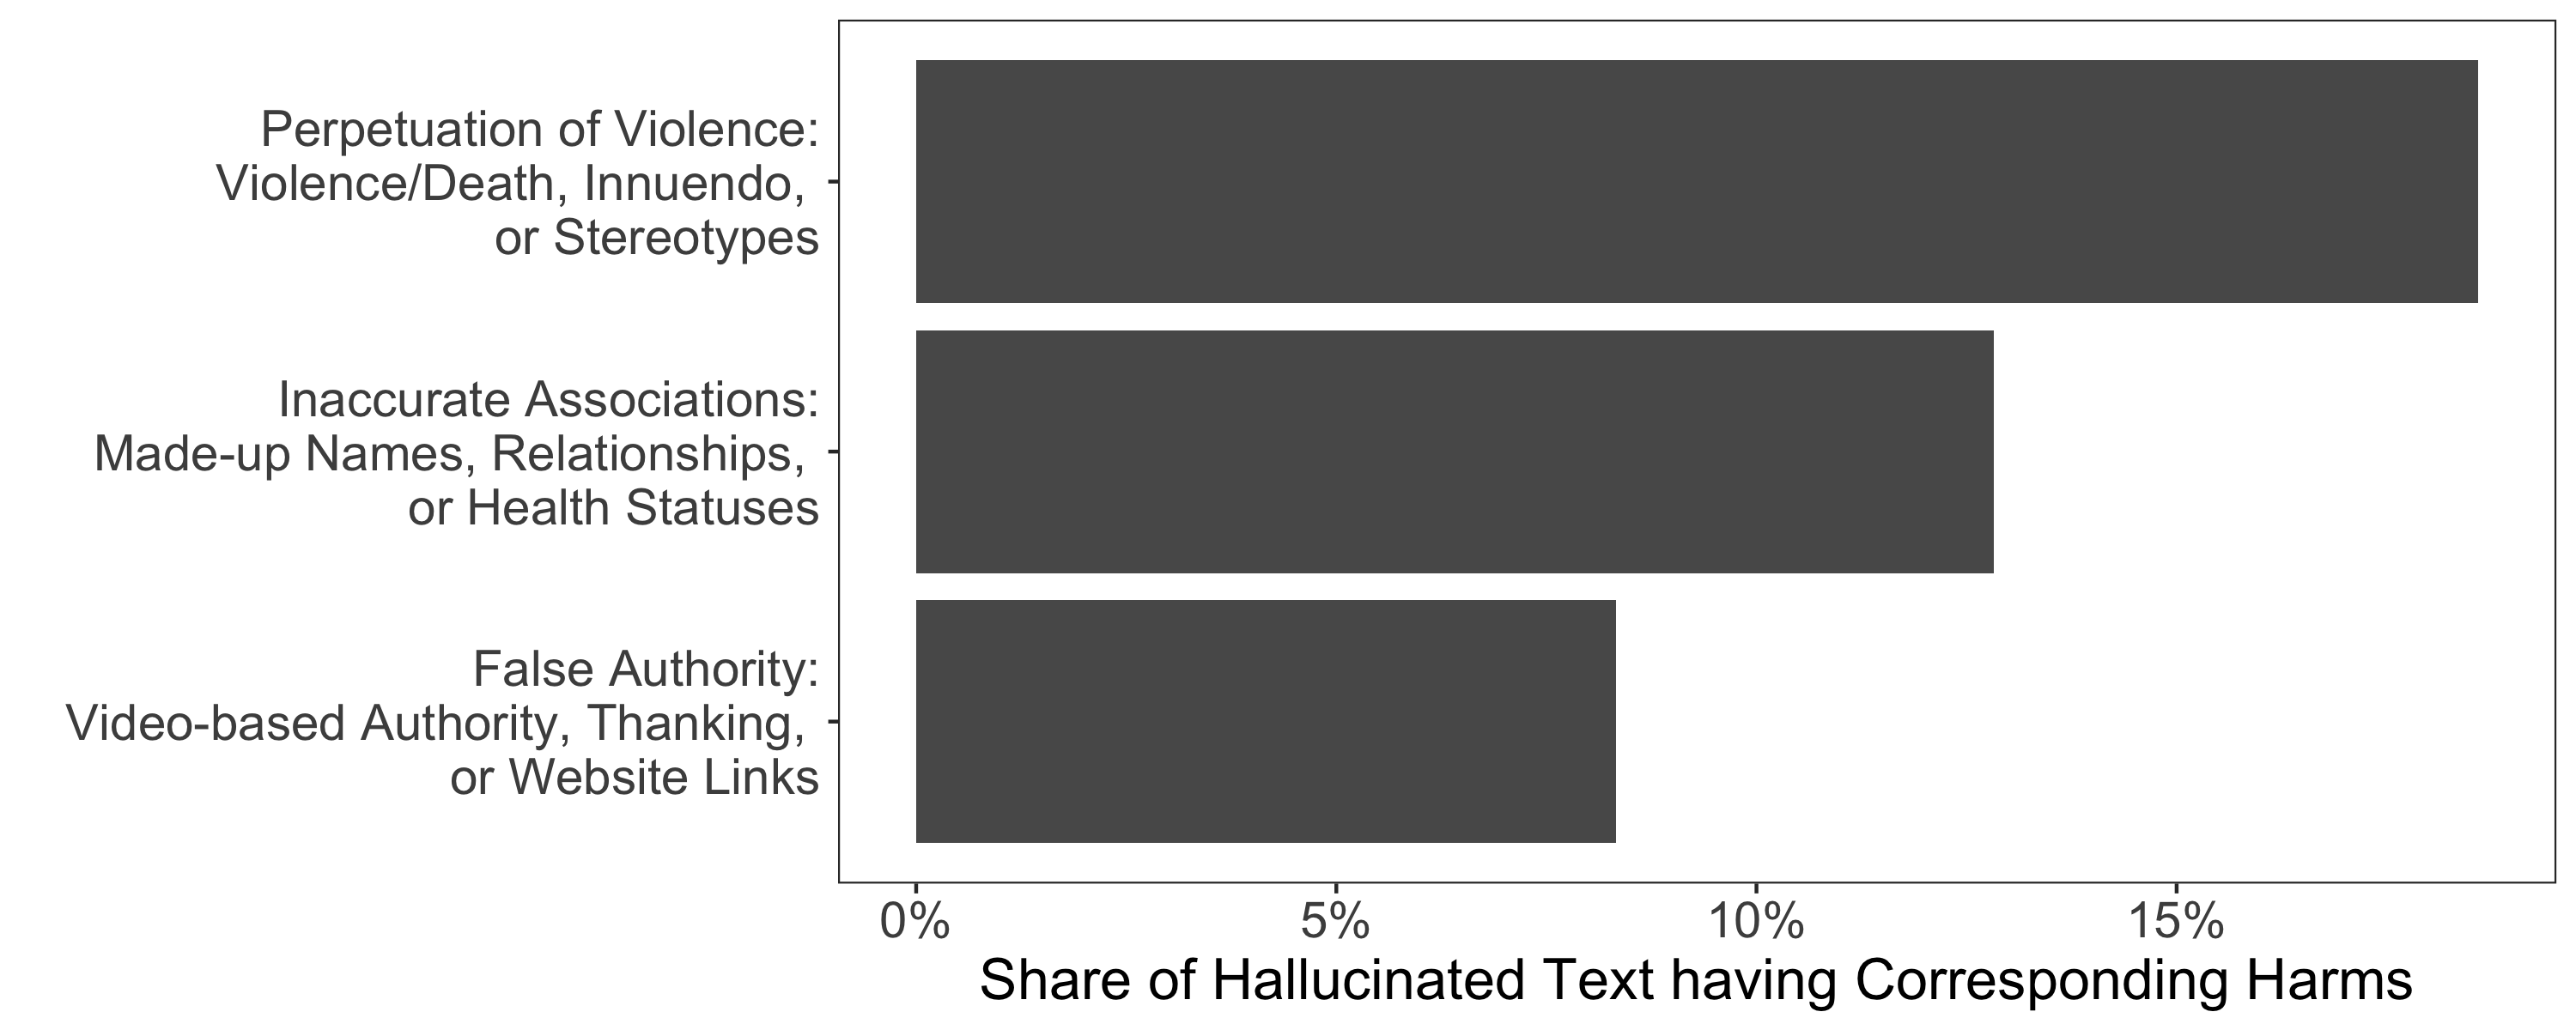
\includegraphics[height=2.3cm]{images2026/careless-whisper-harms.png}
	\vspace*{-0.6em}
	\caption{Types of harm in hallucinated text. Figure from \citep{koenecke2024careless}}
\end{figure}
\end{frame}

%_______________________________________________________

\quizbreak{4}{2}

\section{Talking while listening (full duplex)}

\frame{\tableofcontents[currentsection]}

\begin{frame}
\frametitle{From turn-based to full-duplex dialogue}
\small
\begin{itemize}
	\item \textbf{Cascaded}: VAD + ASR + LLM + TTS ; seconds of latency, paralinguistics lost
	\item \textbf{Half-duplex} speech LLMs (omni models): one turn at a time
	\item \textbf{Full-duplex}: listen \textit{and} speak at the same time, like humans
\end{itemize}
\vspace*{-0.3em}
\begin{center}
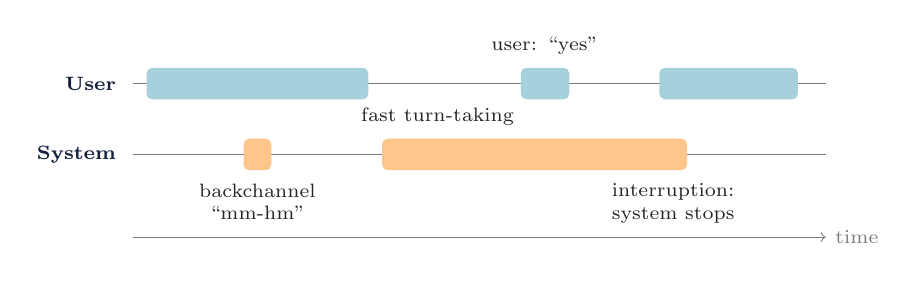
\begin{tikzpicture}[x=0.88cm,y=1cm, every node/.style={font=\scriptsize}]
  \node[anchor=east, font=\scriptsize\bfseries, text=titleink] at (-0.1,0.9) {User};
  \node[anchor=east, font=\scriptsize\bfseries, text=titleink] at (-0.1,0) {System};
  \draw[softgrey] (0,0.9) -- (10,0.9); \draw[softgrey] (0,0) -- (10,0);
  % user speech
  \fill[accent!35, rounded corners=2pt] (0.2,0.7) rectangle (3.4,1.1);
  \fill[accent!35, rounded corners=2pt] (5.6,0.7) rectangle (6.3,1.1);
  \fill[accent!35, rounded corners=2pt] (7.6,0.7) rectangle (9.6,1.1);
  % system speech
  \fill[orange!45, rounded corners=2pt] (1.6,-0.2) rectangle (2.0,0.2);
  \fill[orange!45, rounded corners=2pt] (3.6,-0.2) rectangle (8.0,0.2);
  % annotations
  \node[below, text=ink, align=center] at (1.8,-0.25) {backchannel\\``mm-hm''};
  \node[above, text=ink] at (4.4,0.25) {fast turn-taking};
  \node[above, text=ink] at (5.95,1.15) {user: ``yes''};
  \node[below, text=ink, align=center] at (7.8,-0.25) {interruption:\\system stops};
  \draw[->, softgrey] (0,-1.05) -- (10,-1.05) node[right, text=softgrey] {time};
\end{tikzpicture}
\end{center}
\begin{itemize}
	\item Handle pauses, backchannels, overlaps and interruptions
	\item Two families \citep{chen2025fdsurvey}: \textit{engineered} synchronization (modules decide when to speak) vs. \textit{learned} synchronization (end-to-end)
\end{itemize}
\end{frame}


\begin{frame}
\frametitle{First steps: dGSLM, two speakers at once}
\begin{columns}[T]
\begin{column}{0.62\textwidth}
\small
\begin{itemize}
	\item dGSLM \citep{nguyen2023dgslm}: the first \textit{textless} model of spoken dialogue
	\item Each channel (speaker) turned into HuBERT units ; a dual-tower Transformer with cross-attention models both streams in parallel
	\item Trained on 2,000h of two-channel telephone conversations (Fisher), no text, no labels
	\item Generates laughter, overlaps and natural turn-taking\ldots{} but with little meaning
\end{itemize}
\end{column}
\begin{column}{0.36\textwidth}
\begin{figure}
	\centering
	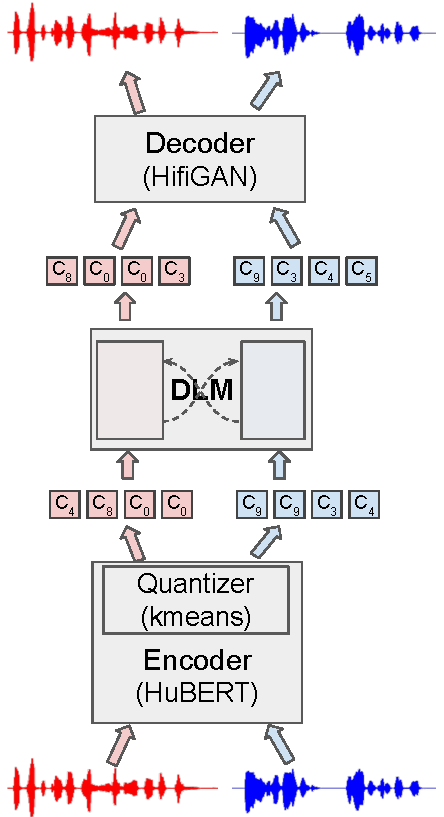
\includegraphics[height=5.6cm]{images2026/dgslm-schema.pdf}
	\caption{Figure from \citep{nguyen2023dgslm}}
\end{figure}
\end{column}
\end{columns}
\end{frame}


% --- SyncLLM slide commented out (uncomment to restore) ---
%\begin{frame}
%\frametitle{SyncLLM: an LLM synchronized with the clock}
%\small
%\begin{itemize}
%	\item SyncLLM \citep{veluri2024syncllm}: Llama-3-8B extended with HuBERT units
%	\item Both speakers interleaved in chunks of 160ms, synchronized with real time
%	\item 212K hours of synthetic dialogues (from text dialogues) + 2K hours of real ones
%\end{itemize}
%\begin{figure}
%	\centering
%	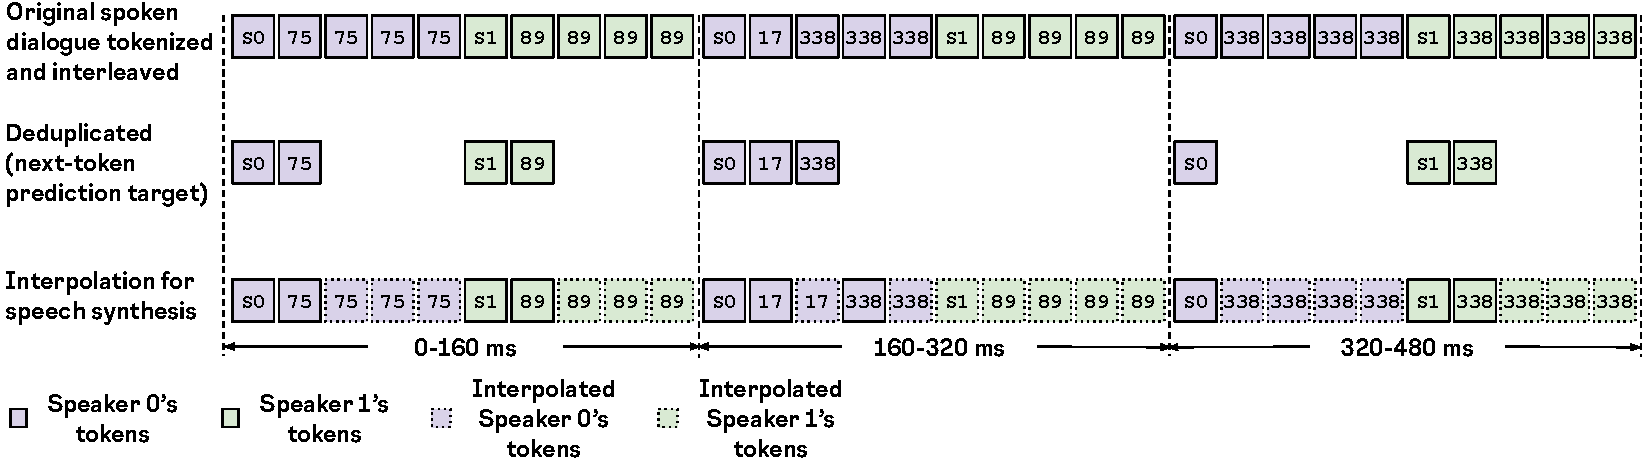
\includegraphics[width=\textwidth]{images2026/syncllm-token-sequence.pdf}
%	\caption{SyncLLM token sequence. Figure from \citep{veluri2024syncllm}}
%\end{figure}
%\end{frame}


\begin{frame}
\frametitle{Moshi \citep{moshi2024}}
\small
\begin{itemize}
	\item First real-time full-duplex spoken LLM: 160ms theoretical latency, 200ms in practice
	\item Speech in and out as Mimi tokens at 12.5Hz (see \textit{Speech as tokens})
	\item \textbf{Multi-stream}: the user's audio and Moshi's own audio are modeled in parallel, no explicit turns
	\item \textbf{Inner monologue}: Moshi also predicts the text of what it says
\end{itemize}
\begin{figure}
	\centering
	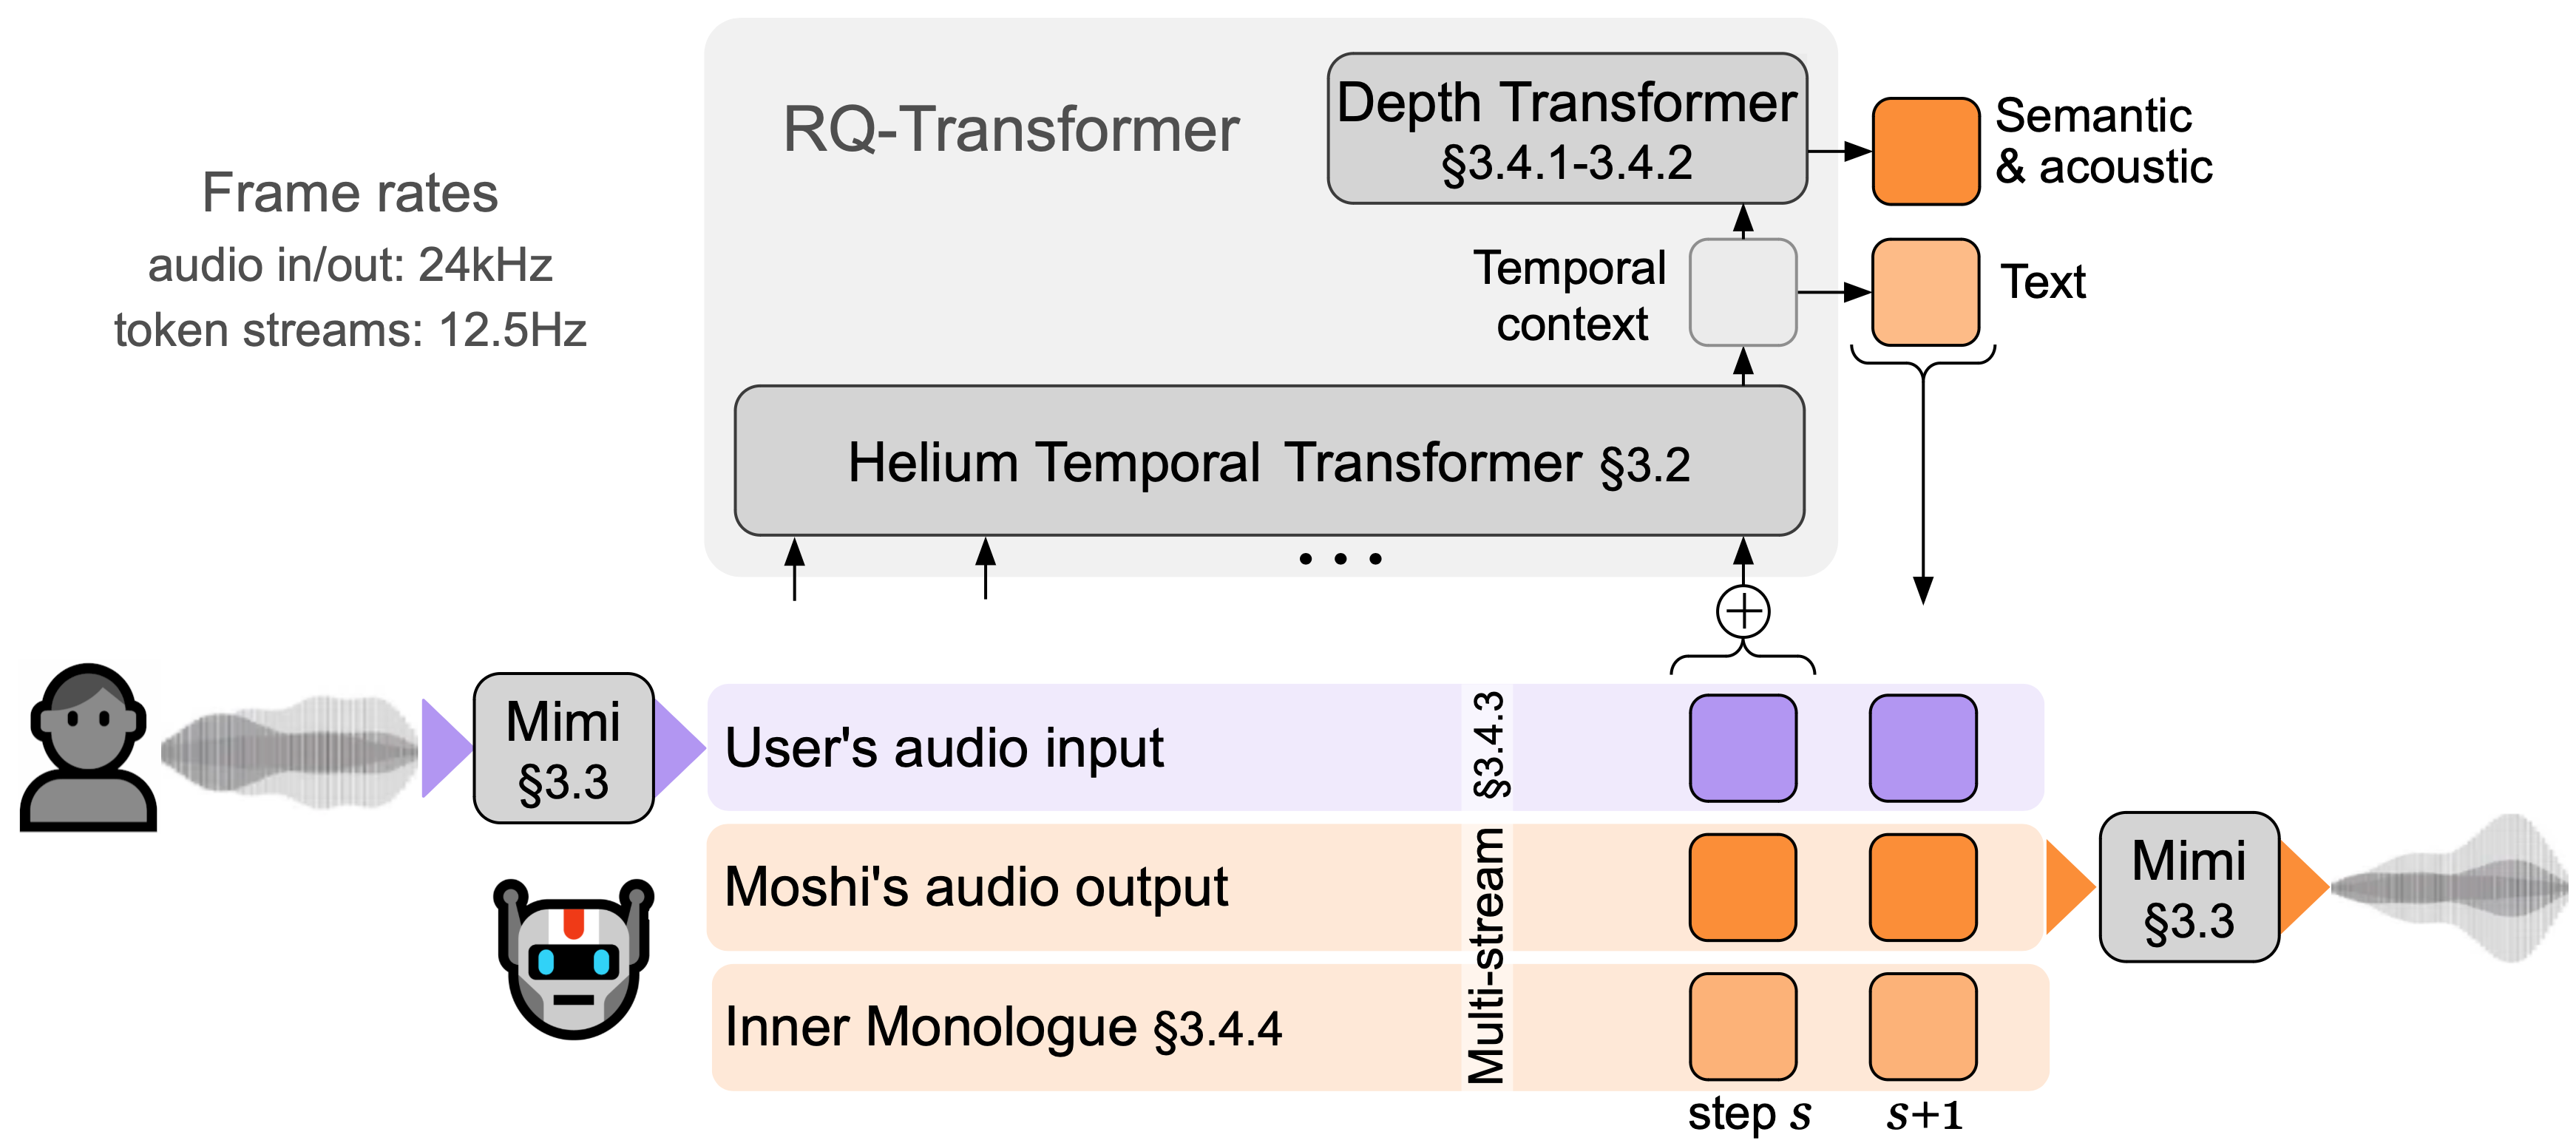
\includegraphics[width=0.68\textwidth]{images2026/moshi-overview-paper.png}
	\caption{Figure from \citep{moshi2024}}
\end{figure}
\end{frame}

\begin{frame}
\frametitle{Moshi: what is modeled at each time step}
\begin{columns}[T]
\begin{column}{0.42\textwidth}
\small
\begin{itemize}
	\item Every 80ms: 8 user tokens (listened), 8 Moshi tokens + 1 text token (generated)
	\item Silence is a token too: Moshi can speak, listen, or both
	\item Text aligned with speech (PAD tokens between words)
	\item Inner monologue: almost $\times$3 spoken QA accuracy
\end{itemize}
\end{column}
\begin{column}{0.56\textwidth}
\begin{figure}
	\centering
	\vspace*{0.5em}
	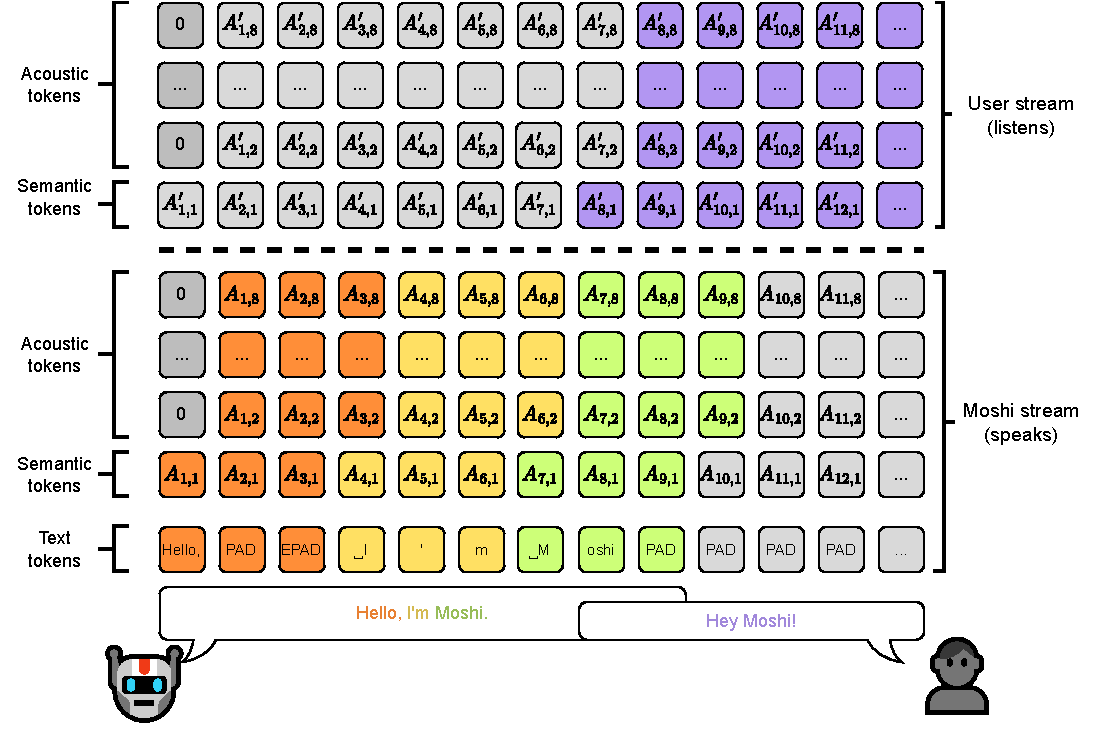
\includegraphics[width=\textwidth]{images2026/moshi-joint-sequence.pdf}
	\caption{Figure from \citep{moshi2024}}
\end{figure}
\end{column}
\end{columns}
\end{frame}

\begin{frame}
\frametitle{Moshi: RQ-Transformer and training}
\begin{columns}[T]
\begin{column}{0.47\textwidth}
\small
\begin{itemize}
	\item \textbf{Temporal Transformer}: Helium, a 7B text LLM (2.1T tokens), over time steps
	\item Small \textbf{Depth Transformer}: the 17 tokens of a step, one after the other
	\item Training: 7M hours of audio (mostly English, Whisper transcripts) ; Fisher for multi-stream ; 20K+ hours of synthetic dialogues with one voice for Moshi
\end{itemize}
\end{column}
\begin{column}{0.51\textwidth}
\begin{figure}
	\centering
	\vspace*{0.8em}
	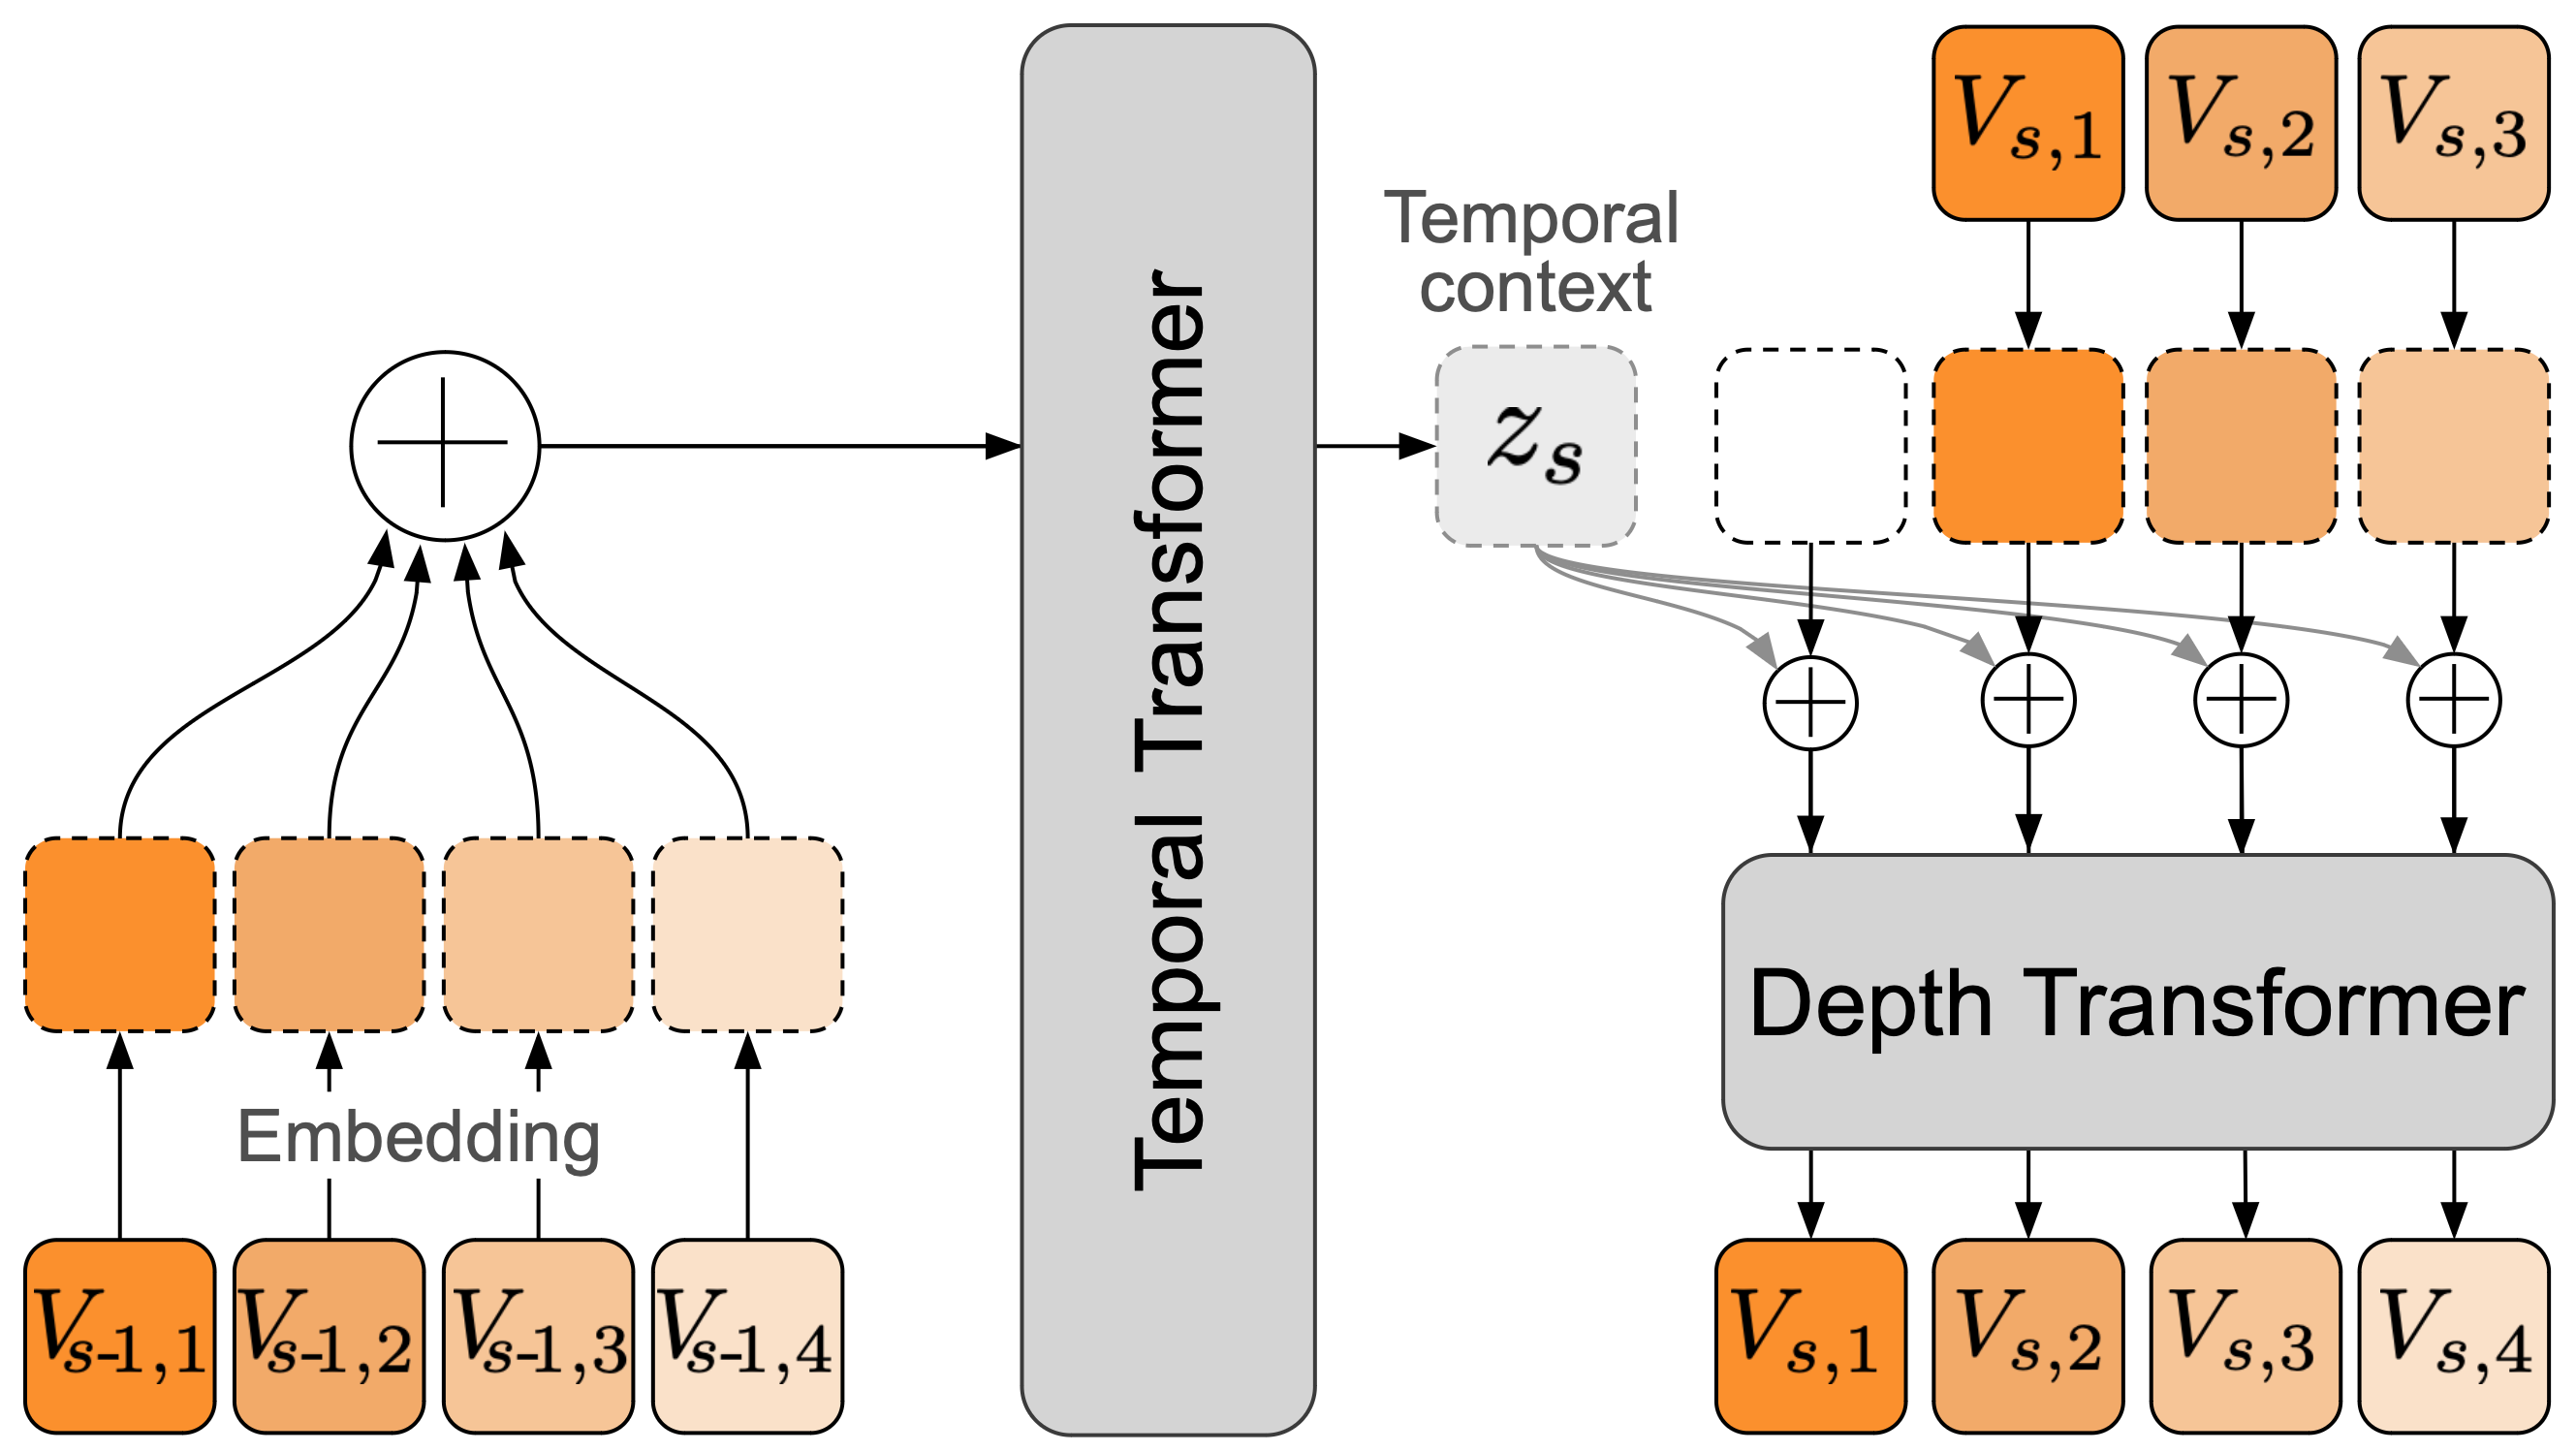
\includegraphics[width=\textwidth]{images2026/moshi-rq-transformer.png}
	\caption{Figure from \citep{moshi2024}}
\end{figure}
\end{column}
\end{columns}
\end{frame}

\begin{frame}
\frametitle{Moshi: performance and limitations}
\begin{itemize}
    \item Outperforms models like SpeechGPT in spoken QA, but loses knowledge compared to Helium (its text LLM)
    \item The same model does streaming ASR (5.7\% WER on Librispeech clean, vs. 3.6\% for a streaming FastConformer) and streaming TTS
    \item Quantization hurts linguistic performance more than audio quality
    \item Open challenges: safety, toxic audio generation, voice misuse
    \item Open model: many successors build on it (PersonaPlex, MoshiRAG\ldots)
\end{itemize}
\end{frame}







% --- old Moshi overview slide (demo photo, source unknown) ---
%\begin{frame}
%\frametitle{Moshi \citep{moshi2024}}
%    \begin{itemize}
%        \item A multi-stream, low-latency speech-to-speech dialogue model
%        \begin{itemize}
%            \item \textbf{Multi-stream}: user and system streams in parallel, no explicit turns
%            \item \textbf{Low-latency}: causal models working on windows of 160ms of speech
%            \item \textbf{Speech-to-speech}: speech in, text and speech out
%            \item \textbf{Dialogue model}: trained mostly on conversational data
%        \end{itemize}
%    \end{itemize}
%    \begin{figure}
%         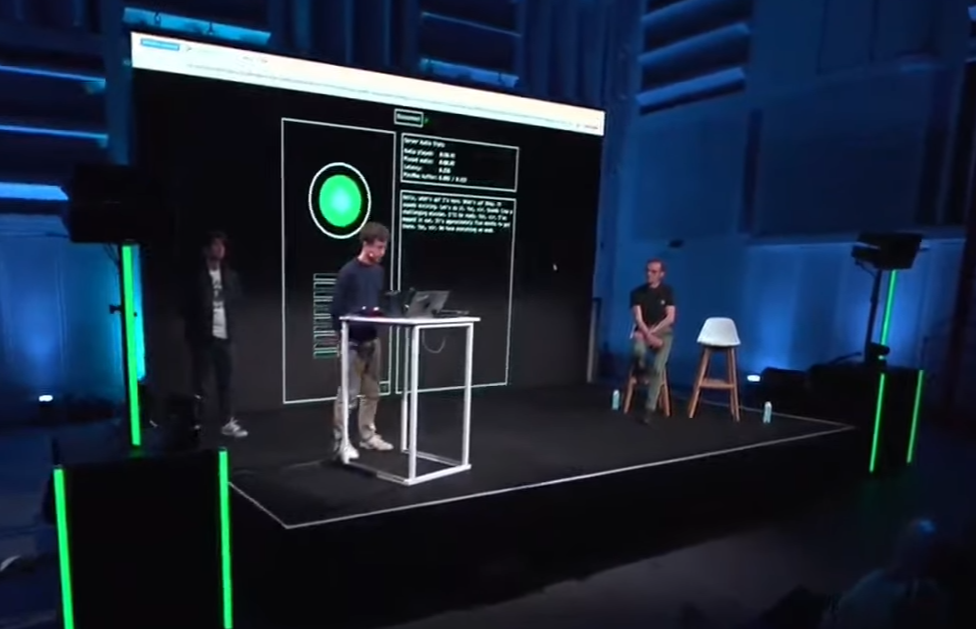
\includegraphics[scale=0.15]{./moshi-0.png}
%    \end{figure}
%\end{frame}

% --- old Moshi architecture slide (figure from Marcely Zanon-Boito) ---
%\begin{frame}
%\frametitle{Moshi: Architecture}
%\begin{columns}
%  \begin{column}{11cm}
%    \begin{itemize}
%        \item At its core is \textbf{Helium}, a 7B parameter text language model (LLM), trained on 2T tokens. The model undergoes specialized training for multistream and full-duplex capabilities.
%        \item Speech in and out as Mimi tokens (see \textit{Speech as tokens})
%             \begin{figure}
%             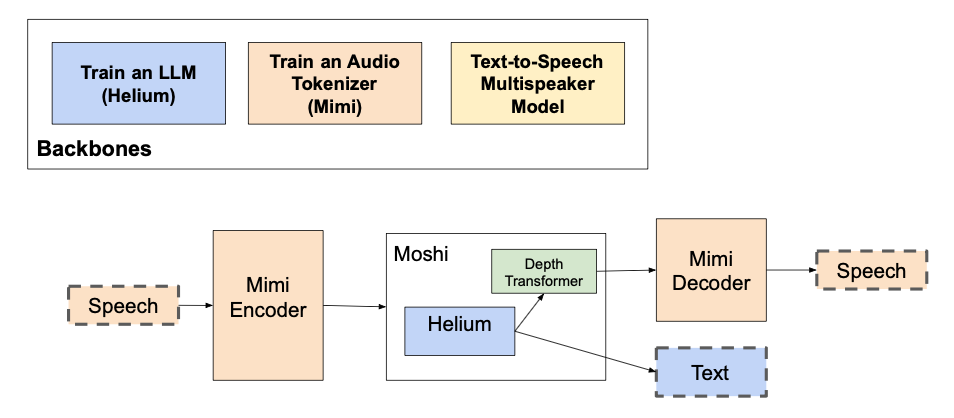
\includegraphics[scale=0.25]{./moshi-overview.png}
%             \caption{Figure from Marcely Zanon-Boito}
%        \end{figure}
%    \end{itemize}
%  \end{column}
%\end{columns}
%\end{frame}


% --- Mimi slide moved to section "Speech as tokens" (old version kept below) ---
%

\begin{frame}
\frametitle{After Moshi (2024-2026)}
\small
\begin{itemize}
	\item \textbf{Frozen or aligned LLMs}: Freeze-Omni \citep{wang2024freezeomni}, MinMo \citep{chen2025minmo} keep the text LLM's knowledge
	\item \textbf{One sequence for both speakers}: OmniFlatten \citep{zhang2024omniflatten} flattens speech and text streams for a GPT-style model
	\item \textbf{No codec inside the LLM}: SALMONN-omni \citep{yu2025salmonnomni} with a ``thinking'' mechanism to decide when to speak or listen ; +30\% relative over open full-duplex models
	\item \textbf{Control}: PersonaPlex \citep{roy2026personaplex} (NVIDIA, fine-tuned from Moshi): role from a text prompt, voice from a speech sample, trained on synthetic dialogues
	\item \textbf{Controllable behaviour}: F-Actor \citep{zuefle2026factor} (next slide)
\end{itemize}
\end{frame}


\begin{frame}
\frametitle{F-Actor: controllable conversational behaviour}
\small
\begin{itemize}
	\item First open, instruction-following full-duplex model trainable on an academic budget \citep{zuefle2026factor}
	\item Instructions control voice, topic, behaviour (number of backchannels, interruptions) and who starts the dialogue
	\item Frozen audio encoder, only the LLM is fine-tuned: 2,000 hours of data, single-stage training ; model and code released
\end{itemize}
\begin{figure}
	\centering
	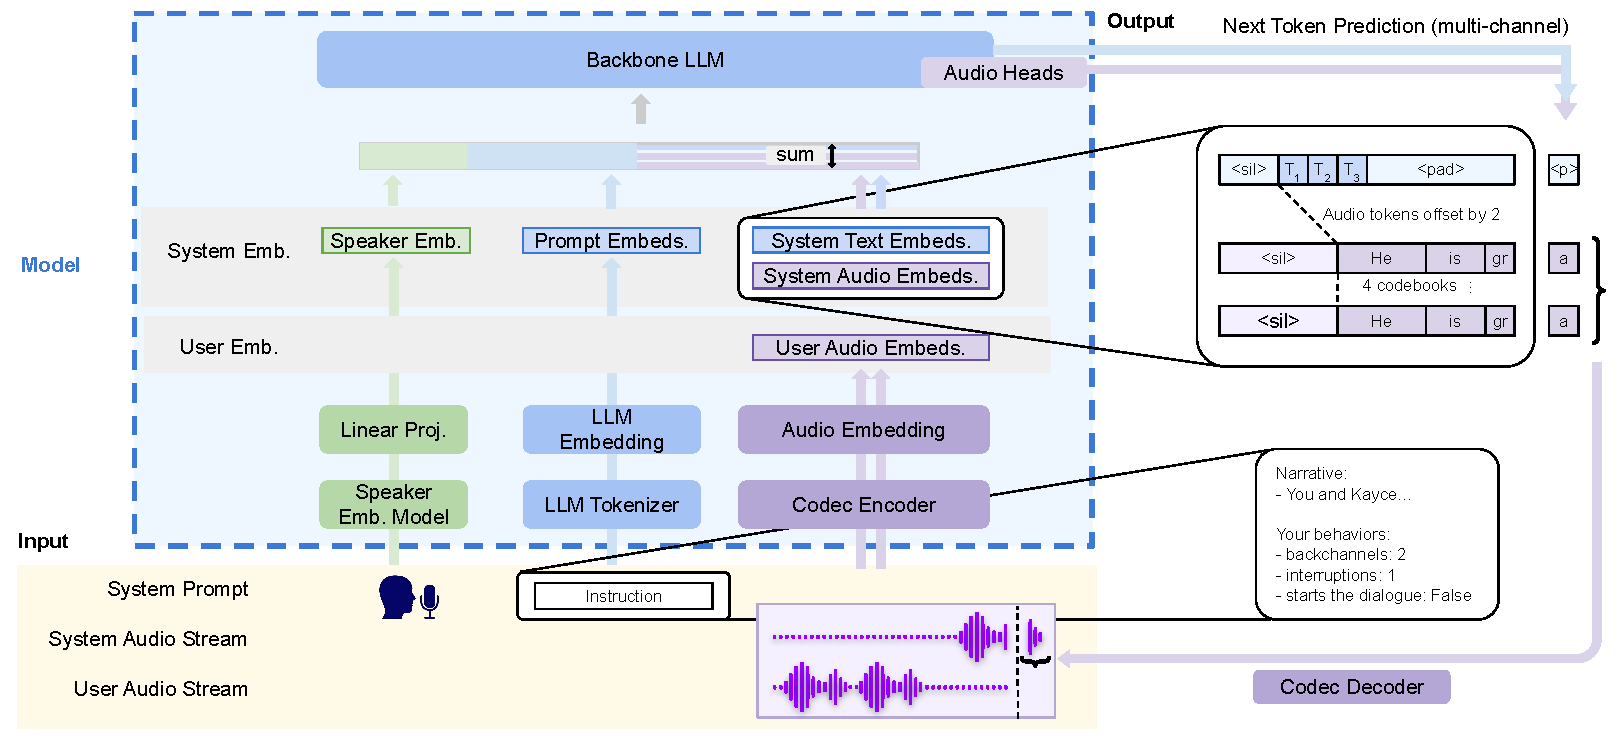
\includegraphics[height=3.5cm]{images2026/factor-overview.pdf}
	\caption{Figure from \citep{zuefle2026factor}}
\end{figure}
\end{frame}


\begin{frame}
\frametitle{Evaluating full-duplex models}
\small
\begin{itemize}
	\item \textbf{Full-Duplex-Bench} \citep{lin2025fdb}: pause handling, backchanneling, turn-taking, interruption management (automatic metrics) ; v2 \citep{lin2025fdbv2}: multi-turn tasks with an automated examiner
	\item \textbf{Talking Turns} \citep{arora2025talkingturns}: a judge model trained on human conversations ; systems often do not know when to speak, interrupt too aggressively and rarely backchannel
	\item \textbf{When to take the floor?} \citep{peng2026takefloor}: models speak when addressed or after silence, but rarely to correct a false claim (14--15\% of replies) or warn of danger (4--7\%)
\end{itemize}
\vspace*{0.5em}
\begin{center}
\fcolorbox{accent}{blockbg}{\begin{minipage}{0.85\textwidth}\centering
Full-duplex models sound natural, but \textit{when} and \textit{what} to say still require real understanding of the conversation
\end{minipage}}
\end{center}
\end{frame}






%_______________________________________________________
\quizbreak{5}{3}

\section{Is ASR solved?}

\frame{\tableofcontents[currentsection]}

\begin{frame}
\frametitle{Is ASR solved?}
\begin{center}
\fcolorbox{accent}{blockbg}{\begin{minipage}{0.9\textwidth}\centering\large
\textbf{Solved as a benchmark, not as a technology for everyone}
\end{minipage}}
\end{center}
\vspace*{0.4em}
\begin{itemize}
	\item[{\color{LigAikumaGreen}\faCheck}] \textbf{Yes}: clean, read or broadcast speech in $\approx$100 well-resourced languages: open models reach $\approx$5\% WER, close to human transcribers, in real time on a laptop
	\item[{\color{red}\faClose}] \textbf{No}: for most of the world's languages, for many speakers (accents, children, atypical speech), in real conversations, and wherever we need to \textit{trust} the output
	\item[{\color{accent}\faArrowRight}] \textbf{And the job has changed}: ASR is now the ears of conversational agents, which must listen \textit{while} speaking
\end{itemize}
\vspace*{0.3em}
{\small Five challenges: languages, speakers, trust, conversations, agents}
\end{frame}


\begin{frame}
\frametitle{Challenge 1: the long tail of languages}
\begin{columns}[T]
\begin{column}{0.56\textwidth}
\small
\begin{itemize}
	\item 7,000+ languages ; supported: Whisper 99 \citep{whisper}, USM 100+ \citep{zhang2023usm}, MMS 1,100+ \citep{pratap2023mms}, Omnilingual 1,600+ \citep{omnilingual2025}
	\item Very uneven quality: Whisper large-v3 from $\approx$3\% to 50\%+ error rate
	\item Still open: dialects, code-switching, unwritten languages
\end{itemize}
\end{column}
\begin{column}{0.42\textwidth}
\begin{figure}
	\centering
	\vspace*{1em}
	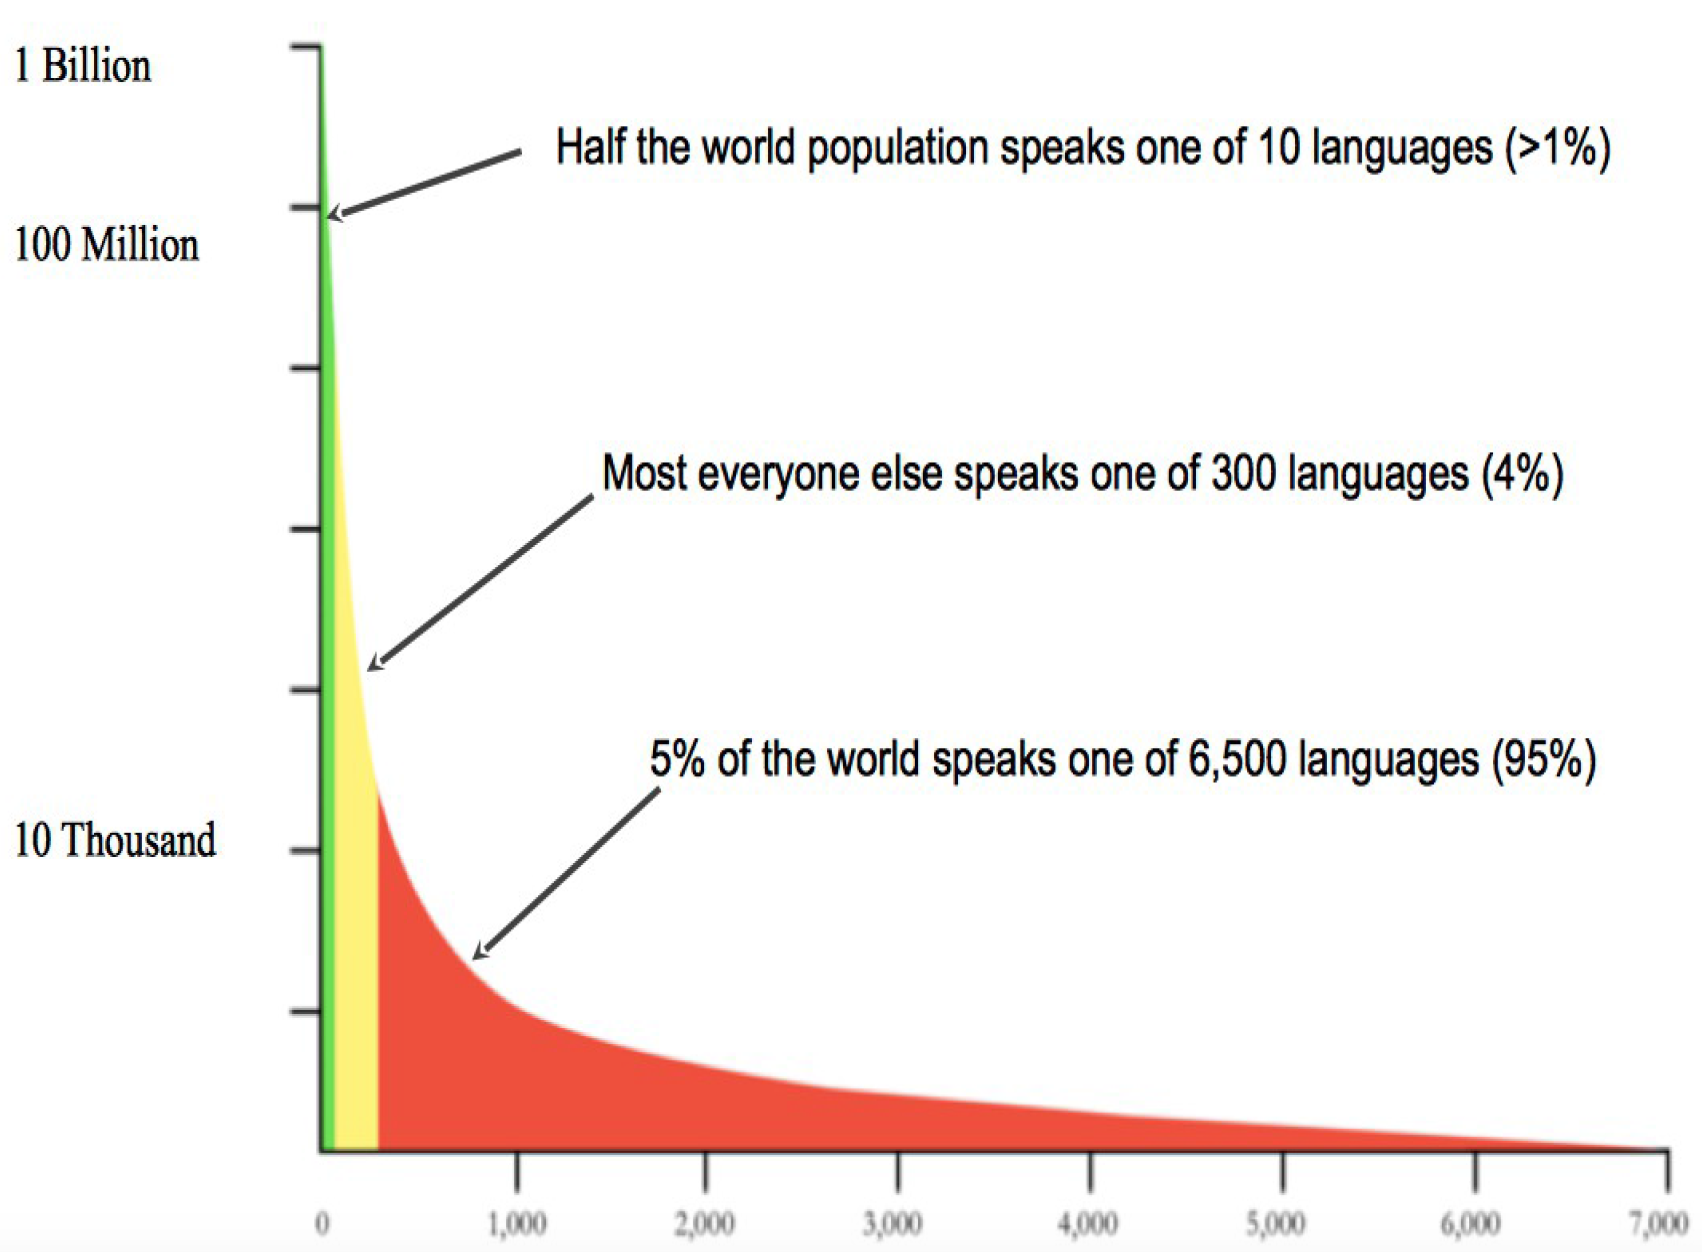
\includegraphics[width=\textwidth]{longtail.png}
	\caption{from Laura Welcher - Big Data for Small Languages \- The Rosetta Project}
\end{figure}
\end{column}
\end{columns}
\end{frame}


\begin{frame}
\frametitle{Challenge 2: not all speakers are equal}
\small
\begin{itemize}
	\item ``Human parity'' on Switchboard in 2016 \citep{xiong2016parity}\ldots{} but not for everyone
	\item Accented speech: much larger gap between humans and machines (table)
	\item Stuttered and dysarthric speech: WER 2--5$\times$ higher than on the leaderboard, up to 24$\times$ with hallucination bursts \citep{dhaka2026werarewe} ; more hallucinations for speakers with aphasia \citep{koenecke2024careless}
	\item Children, elderly, non-native speakers: under-represented ; report results per group
\end{itemize}
\vspace*{-0.4em}
\begin{figure}
	\centering
	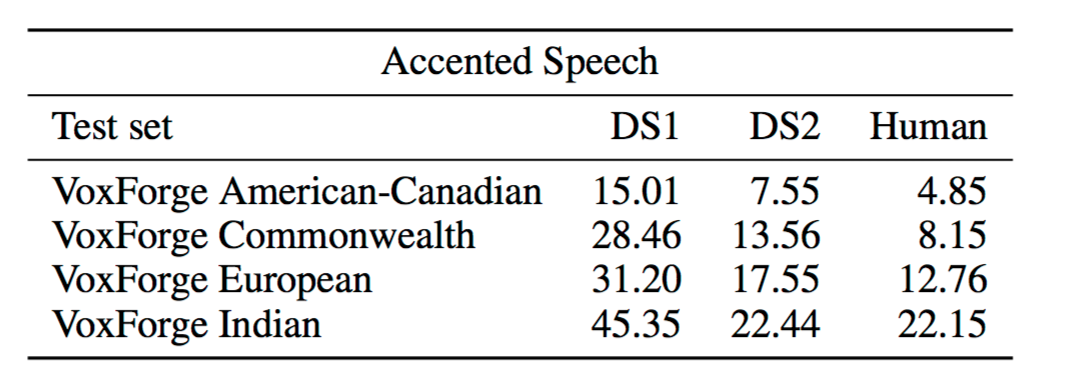
\includegraphics[width=0.5\textwidth]{superhuman2.png}
	\vspace*{-0.6em}
	\caption{Accented speech, table from \citep{DBLP:conf/icml/AmodeiABCCCCCCD16}}
\end{figure}
\end{frame}


\begin{frame}
\frametitle{Challenge 3: trust and evaluation beyond WER}
\small
\begin{itemize}
	\item Standard benchmarks saturate: $\approx$5\% average WER for the best systems
	\item Hallucinations: fluent, invented text ($\approx$1\% of Whisper transcriptions, 38\% of them harmful \citep{koenecke2024careless})
	\item WER treats all errors the same:
\end{itemize}
\begin{center}
\renewcommand{\arraystretch}{1.2}
\begin{tabular}{llcl}
	\textbf{REF} & do not take this medicine & & \\
	\hline
	HYP A & do not take {\color{orange}these} medicine & WER 20\% & {\color{LigAikumaGreen}meaning kept} \\
	HYP B & do {\color{red}--} take this medicine & WER 20\% & {\color{red}meaning reversed} \\
\end{tabular}
\end{center}
\begin{itemize}
	\item Towards: semantic metrics (e.g. BERTScore), errors on names and keywords, hallucination rates, LLM judges, task success
\end{itemize}
\end{frame}


\begin{frame}
\frametitle{Challenge 4: real conversations}
\small
\begin{itemize}
	\item Overlapping speech, many speakers, far-field microphones, long recordings
	\item ``Who said what, when'': ASR + diarization, e.g. distant meeting transcription in NOTSOFAR-1 \citep{vinnikov2024notsofar}
	\item Long-form audio: the same models make 1.5--2$\times$ more errors ; LLM decoders also get much slower (Canary-Qwen: RTFx 418 $\rightarrow$ 16)
\end{itemize}
\begin{center}
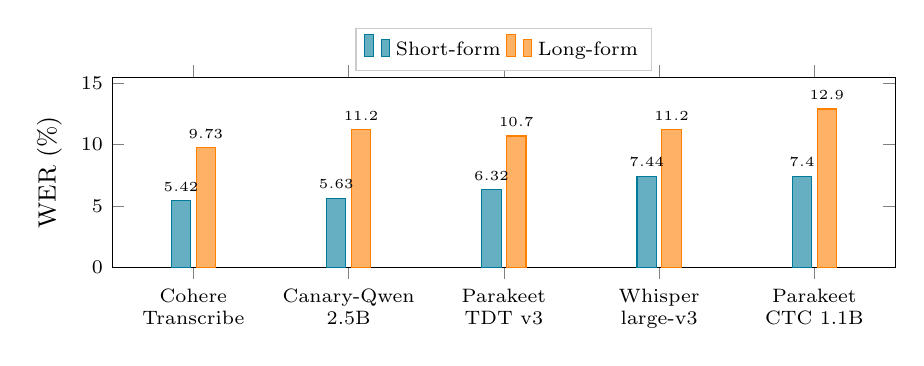
\begin{tikzpicture}
\begin{axis}[
  ybar, bar width=7pt, width=0.95\textwidth, height=4.0cm,
  ymin=0, ymax=15.5, ylabel={\small WER (\%)},
  symbolic x coords={Cohere Transcribe,Canary-Qwen 2.5B,Parakeet TDT v3,Whisper large-v3,Parakeet CTC 1.1B},
  xtick=data, xticklabels={Cohere\\Transcribe,Canary-Qwen\\2.5B,Parakeet\\TDT v3,Whisper\\large-v3,Parakeet\\CTC 1.1B}, xticklabel style={font=\scriptsize, align=center},
  tick label style={font=\scriptsize},
  legend style={font=\scriptsize, at={(0.5,1.03)}, anchor=south, draw=gray!40, legend columns=2},
  nodes near coords, every node near coord/.append style={font=\tiny},
  enlarge x limits=0.13,
]
\addplot[fill=accent!60, draw=accent] coordinates {(Cohere Transcribe,5.42) (Canary-Qwen 2.5B,5.63) (Parakeet TDT v3,6.32) (Whisper large-v3,7.44) (Parakeet CTC 1.1B,7.40)};
\addplot[fill=orange!60, draw=orange] coordinates {(Cohere Transcribe,9.73) (Canary-Qwen 2.5B,11.2) (Parakeet TDT v3,10.7) (Whisper large-v3,11.2) (Parakeet CTC 1.1B,12.9)};
\legend{Short-form, Long-form}
\end{axis}
\end{tikzpicture}

{\footnotesize\color{softgrey} Data from \citep{srivastav2025openasr}}
\end{center}
\end{frame}


\begin{frame}
\frametitle{Challenge 5: ASR inside conversational agents}
\small
\begin{itemize}
	\item \textbf{ASR is the ears of agents}: errors propagate to actions
	\item \textbf{Speed}: humans leave $\approx$200ms between turns \citep{stivers2009universals} ; voice agents calling tools still need 4--10s \citep{lin2026fdbv3}
	\item \textbf{Full duplex}: listen while speaking (echo, barge-in), know \textit{when} to speak \citep{peng2026takefloor}, keep the LLM's knowledge
	\item \textbf{Streaming, on-device} ASR: privacy, cost
	\item \textbf{Multimodal, multi-party conversation} (embodied AI, robots)
	\begin{itemize}
		\item who is speaking, and \textit{to whom}? gaze, head pose, body posture \citep{mazzola2023addressee}
		\item hard for LLMs: GPT-4o barely above chance on three-party addressee recognition \citep{inoue2025addressee} ; multimodal LLMs below humans \citep{fukuda2026addressee}
		\item first audio-visual full-duplex models \citep{huang2026duplexomni}
	\end{itemize}
\end{itemize}
\end{frame}

% --- old slide commented out: Remaining challenges in 2026 ---
%\begin{frame}
%	\frametitle{Remaining challenges in 2026}
%	\begin{itemize}
%		\item \textbf{Languages}: 1,600+ languages covered \citep{omnilingual2025} out of $\approx$7,000, with very uneven quality
%		\item \textbf{Nonstandard speech}: stuttering, dysarthria, accents, children, elderly speakers
%		\item \textbf{Hallucinations}: fluent, wrong, sometimes harmful outputs
%		\item \textbf{Conversational and long-form speech}: overlaps, many speakers, far-field microphones
%		\item \textbf{Efficiency}: streaming, on-device, low latency
%		\item \textbf{Evaluation}: WER on standard benchmarks saturates ($\approx$5\%) ; we need task- and user-centred metrics
%		\item \textbf{Beyond transcription}: understanding, dialogue, useful full-duplex agents
%	\end{itemize}
%\end{frame}

% --- old challenges slide (o1-generated image) commented out ---
%\begin{frame}
%	\frametitle{ASR Remaining Challenges in 2024}
%%From Baidu's Deep Speech paper \citep{DBLP:conf/icml/AmodeiABCCCCCCD16}
%	
%			\begin{figure}
%			\centering
%			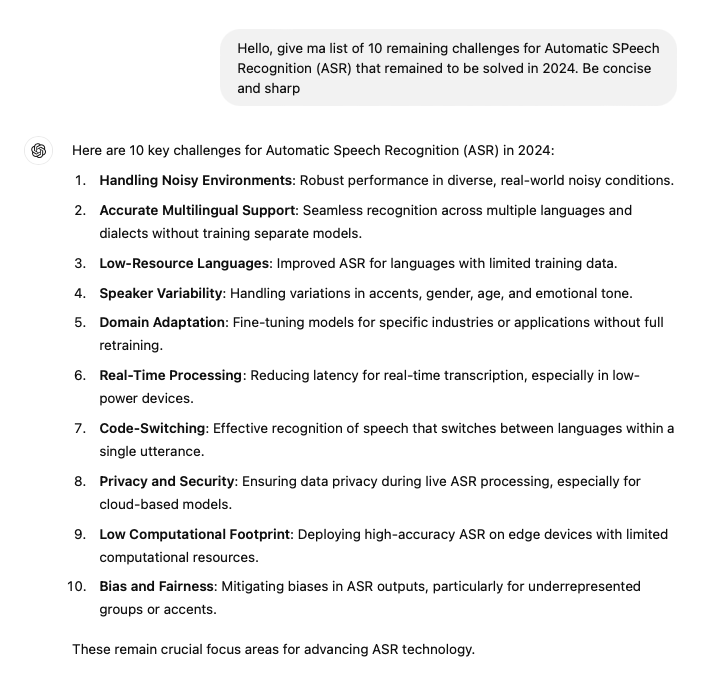
\includegraphics[scale=0.25]	{challenges2024.png} 
%		%	[scale=0.35,trim=0mm 140mm 0mm 0mm,clip=true]
%			\caption{ASR challenges in 2024 according to openai o-1 }
%			\label{fig:challenges}
%			\end{figure}	
%	
%\end{frame}


% --- old slide commented out: Language coverage ---
%\begin{frame}
%	\frametitle{Language coverage}
%	\small
%		\begin{itemize}
%			\item $\approx$7,000 languages spoken in the world ; 300 languages cover 95\% of the population ; more than 6,000 raise documentation and revitalisation issues
%			\item Whisper: 99 languages \citep{whisper} ; Google USM: 100+ (pre-trained on 300+) \citep{zhang2023usm} ; MMS: 1,100+ \citep{pratap2023mms} ; Omnilingual ASR: 1,600+ \citep{omnilingual2025}
%		\end{itemize}
%			\begin{figure}
%			\centering
%			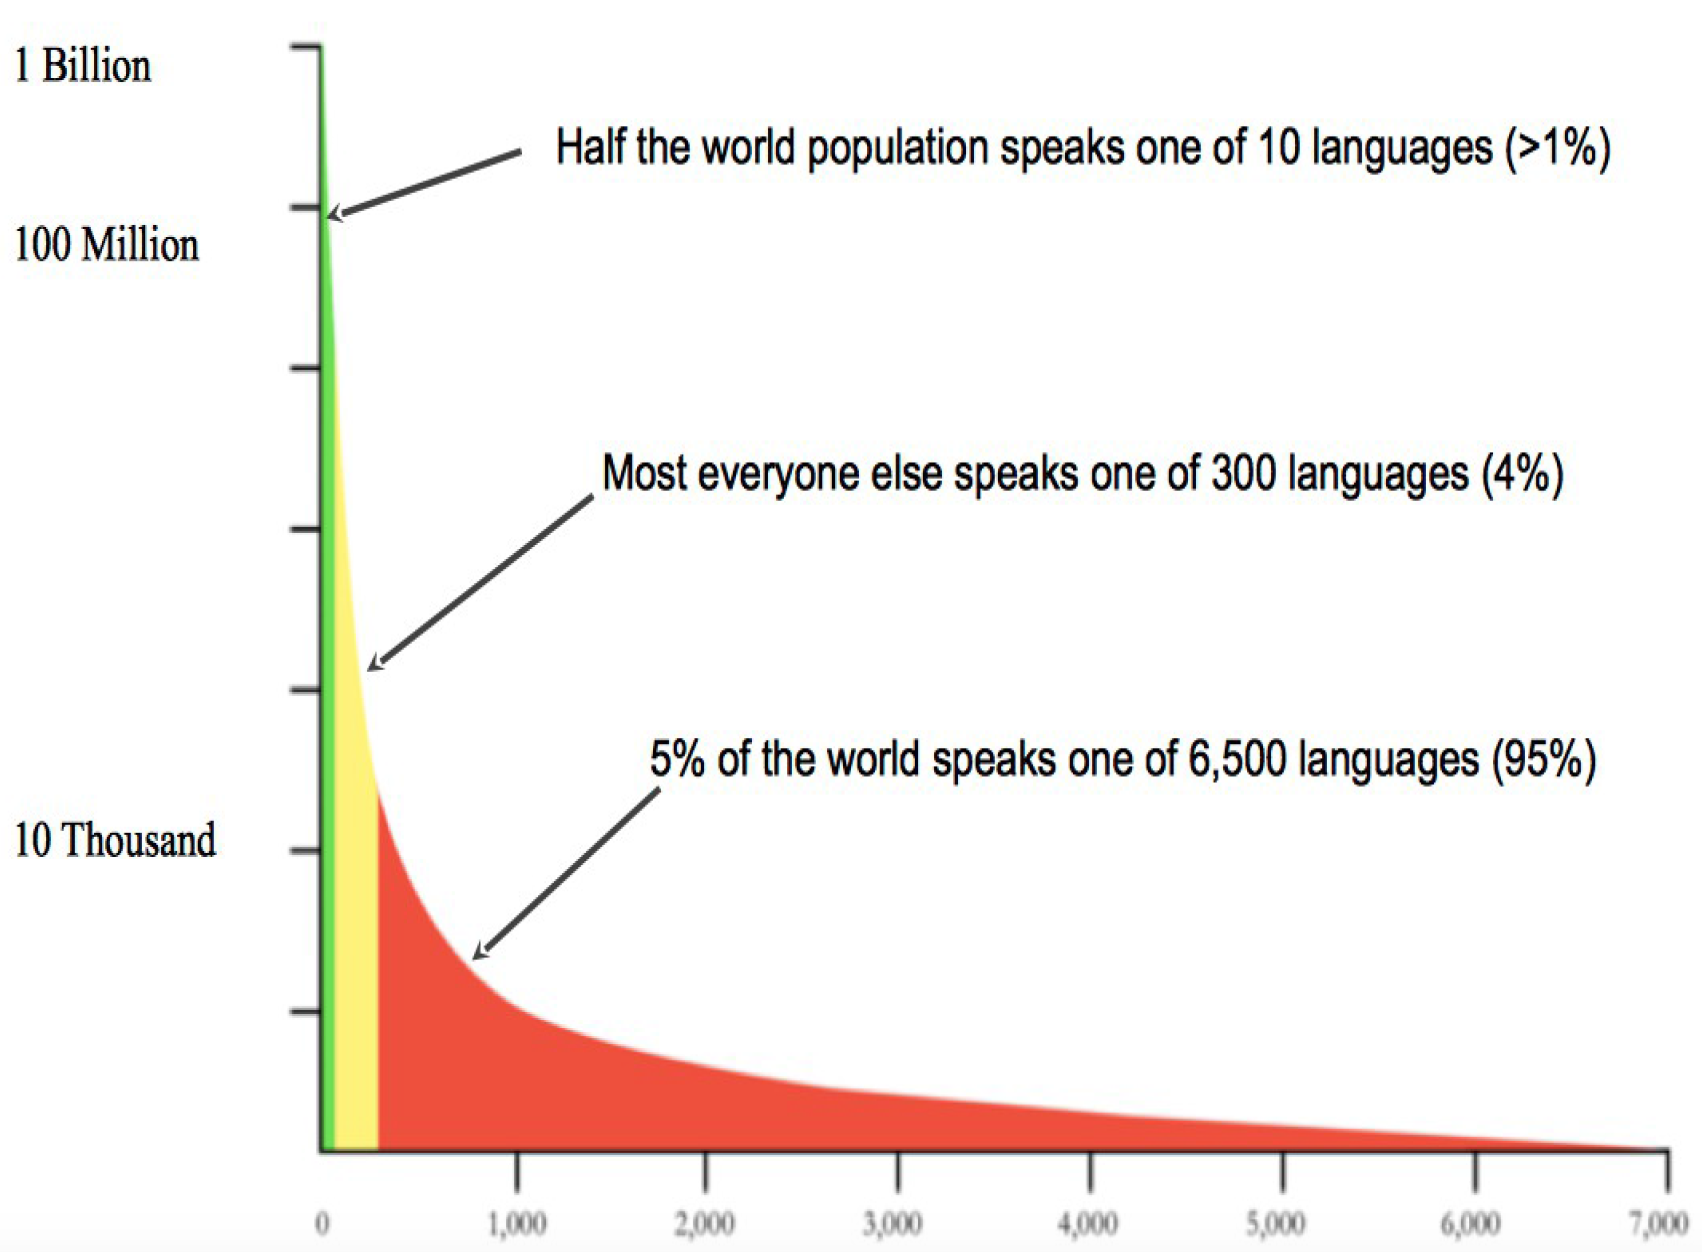
\includegraphics[height=3.3cm]	{longtail.png} 
%			\caption{from Laura Welcher - Big Data for Small Languages \- The Rosetta Project}
%			\label{fig:longtail}
%			\end{figure}
%\end{frame}

% --- old slide commented out: Low resource ASR ---
%\begin{frame}
%	\frametitle{Low resource ASR}
%\begin{columns}[T]
%\begin{column}{0.42\textwidth}
%\small
%\begin{itemize}
%	\item Even a model trained on 5M hours is very uneven across languages
%	\item Whisper large-v3: from $\approx$3\% to 50\%+ error rate depending on the language
%	\item Low-resource languages remain far behind
%\end{itemize}
%\end{column}
%\begin{column}{0.56\textwidth}
%			\begin{figure}
%			\centering
%			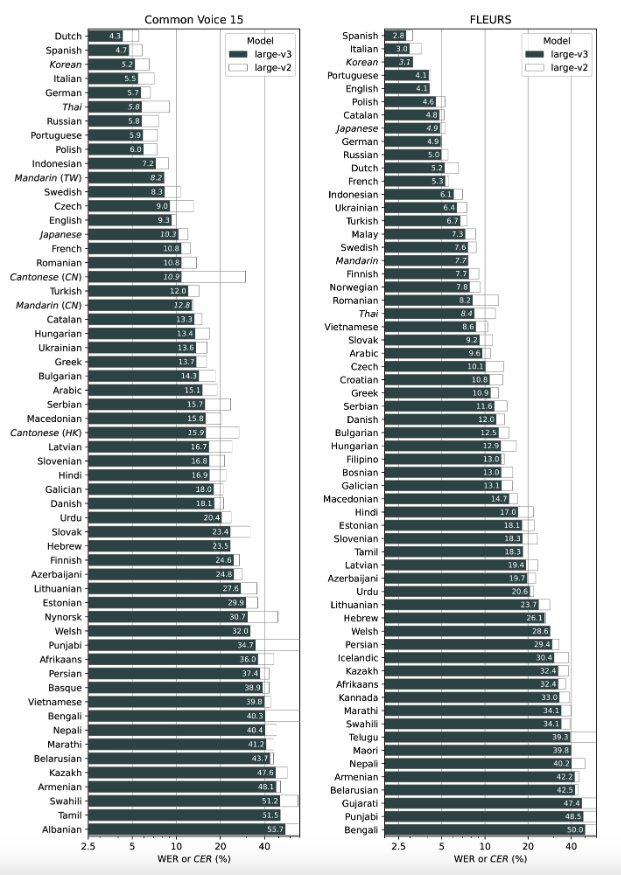
\includegraphics[height=5.9cm]	{low-resoiurce-asr.png} 
%			\vspace*{-0.6em}
%			\caption{Whisper large-v3 vs. large-v2. Figure from the large-v3 release {\tiny\url{https://github.com/openai/whisper/discussions/1762}}}
%			\label{fig:lowresourceASR}
%			\end{figure}
%\end{column}
%\end{columns}
%\end{frame}

% --- old slide commented out: On par with human transcription? ---
%\begin{frame}
%	\frametitle{On par with human transcription?}
%	\small
%	\begin{itemize}
%		\item 2016: ``human parity'' on Switchboard: 5.8\% WER vs. 5.9\% for professional transcribers \citep{xiong2016parity}
%		\item 2016: Deep Speech 2 close to humans on read speech, not on accented or noisy speech \citep{DBLP:conf/icml/AmodeiABCCCCCCD16}
%		\item 2026: best open models reach 5--7\% WER on standard benchmarks, but 2--5$\times$ more on stuttered and dysarthric speech, up to 24$\times$ with hallucination bursts \citep{dhaka2026werarewe}
%	\end{itemize}
%			\begin{figure}
%			\centering
%			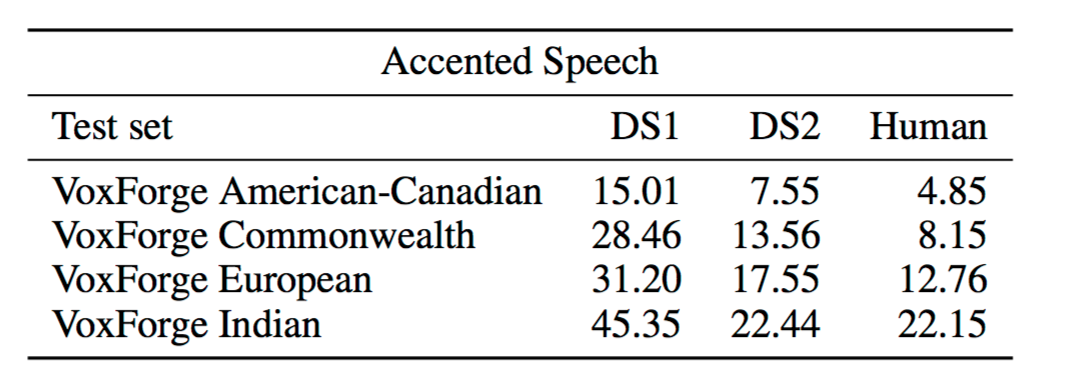
\includegraphics[width=0.75\textwidth]	{superhuman2.png} 
%			\caption{Human vs. machine WER on \textbf{accented} speech (from \citep{DBLP:conf/icml/AmodeiABCCCCCCD16})}
%			\label{fig:superhuman2}
%			\end{figure}
%\end{frame}

% --- old slide commented out: Zero resource ASR ---
%\begin{frame}
%	\frametitle{Zero resource ASR}
%	\small
%In an unknown language, from unannotated raw speech, discover:\footnote{The zero resource challenge: \url{http://zerospeech.com} \citep{DBLP:journals/corr/abs-1712-04313}}
%		\begin{itemize}
%			\item Invariant subword units (phone units ?) and words/terms (lexicon/semantic units ?)
%		\end{itemize}
%Technological challenge
%		\begin{itemize}
%			\item Can we build useful speech technologies without any textual resources ?
%			\item Unsupervised ASR now works: wav2vec-U \citep{baevski2021wav2vecu} maps SSL representations to phonemes with unpaired text (TIMIT phone error rate 26.1 $\rightarrow$ 11.3)
%			\item Textless spoken language models: GSLM \citep{lakhotia2021gslm}, dGSLM \citep{nguyen2023dgslm}
%		\end{itemize}
%Scientific challenge
%		\begin{itemize}
%			\item Can we build algorithms that learn languages like infants do ?
%		\end{itemize}
%\end{frame}



\begin{frame}{Resources}
\small
\begin{itemize}
    \item Follow me on Twitter/X: \href{https://x.com/laurent_besacie}{Go to @laurent\_besacie}
    \item Blog on Multimodal Speech-Text Models: \href{https://europe.naverlabs.com/blog/on-multimodal-speech-text-pre-trained-models/}{Read the Blog Post}
    \item Research on Multimodal NLP for Robotics: \href{https://europe.naverlabs.com/research/multimodal-nlp-for-robotics/}{Read Naver Labs Research Page on Multimodal NLP for Robotics}
    \item Notebook (in French) on ASR and Multimodal Foundation Models:  \href{https://colab.research.google.com/drive/13-qJfsHvVZNQ6SSBR3ULZw0HOqe05OwO?usp=sharing}{Link}
    \item Open ASR Leaderboard: \href{https://huggingface.co/spaces/hf-audio/open_asr_leaderboard}{huggingface.co/spaces/hf-audio/open\_asr\_leaderboard}
    \item Curated list of full-duplex models and benchmarks: \href{https://github.com/Ruiqi-Yan/Awesome-Full-Duplex-SDM}{github.com/Ruiqi-Yan/Awesome-Full-Duplex-SDM}
    \item Hugging Face Audio Course (hands-on ASR, Whisper fine-tuning, TTS): \href{https://huggingface.co/learn/audio-course}{huggingface.co/learn/audio-course}
    \item Moshi code and models: \href{https://github.com/kyutai-labs/moshi}{github.com/kyutai-labs/moshi}
\end{itemize}
\end{frame}

\begin{frame}
	\frametitle{Questions?}
	
	\vfill
	\centerline{\Huge Thank you}
	\vfill
\end{frame}







%_______________________________________________________





\ifquiz
\begin{frame}
\frametitle{Quiz answers}
\scriptsize
\vspace*{-0.4em}
\begin{columns}[T]
\begin{column}{0.49\textwidth}
\textbf{\color{accent}Break 1: From waves to words}
\begin{itemize}\setlength\itemsep{0pt}
	\item p(w) is modeled by $\rightarrow$ the language model
	\item WER $>$ 100\% because of $\rightarrow$ insertions
	\item Languages you speak at home $\rightarrow$ (word cloud)
\end{itemize}
\textbf{\color{accent}Break 2: Going end-to-end}
\begin{itemize}\setlength\itemsep{0pt}
	\item One label per frame + ``blank'' $\rightarrow$ CTC
	\item Fastest decoders on the leaderboard $\rightarrow$ CTC and TDT (transducer)
	\item Speech recognition you have used $\rightarrow$ (poll)
\end{itemize}
\textbf{\color{accent}Break 3: SSL and speech tokens}
\begin{itemize}\setlength\itemsep{0pt}
	\item SSL harder for speech $\rightarrow$ continuous signal: no fixed vocabulary, no word boundaries
	\item HuBERT predicts for masked frames $\rightarrow$ discrete cluster IDs (hidden units)
	\item Last RVQ codebooks encode $\rightarrow$ fine details (what is left)
\end{itemize}
\end{column}
\begin{column}{0.49\textwidth}
\textbf{\color{accent}Break 4: When LLMs learn to listen}
\begin{itemize}\setlength\itemsep{0pt}
	\item The adapter $\rightarrow$ reduces the frame rate and maps audio features to the LLM space
	\item Typical risk of LLM-based ASR $\rightarrow$ inventing fluent text not in the audio (hallucination)
\end{itemize}
\textbf{\color{accent}Break 5: Talking while listening}
\begin{itemize}\setlength\itemsep{0pt}
	\item Moshi is full duplex because $\rightarrow$ it models the user's and its own audio streams in parallel
	\item Moshi's inner monologue $\rightarrow$ time-aligned text tokens predicted with its own speech
	\item What annoys you most with voice assistants $\rightarrow$ (poll)
\end{itemize}
\end{column}
\end{columns}
\end{frame}
\fi

\begin{frame}[allowframebreaks]
        \frametitle{References}
        {\scriptsize
        \bibliographystyle{apalike}
        \bibliography{laurent,laurent2,mybib,refs,./bibs/refs2,./bibs/refs2026}}
        %\bibliography{laurent}}
\end{frame}    





\end{document}







